%%%%%%%%%%%%%%%%%%%%%%%%%%%%%%%%%%%%%%%%%%%%%%%%%%%%%%%%%%%%%%%%%%%%%%
% All the option for the style report can be used (e.g. twoside, ....
% Moreover, the following options are also available: french, UOdraft,
% hyperref, ...
%
% The options french and UOdraft do not need any explanation.  You may want
% to add the option twoside to the option UOdraft to further reduce the
% number of pages.
%
% The option  hyperref is for those who would like to use the package
% hyperref.sty .
%
% Avec l'option  french , il est possible de compiler un texte qui
% possede des accents, ... sans avoir a recourir aux symboles \'e,
% \"u, etc.  En plus de permettre l'utilisation d'un editeur de texte
% normal, vous pouvez aussi utiliser votre "spell checker" prefere.
%
% With the option NoTofC, the section for the list of symbols isn't
% included in the table of Contents.  The default is that it is
% included in the list of contents.
%
% To compile the template, on has to do something like
%
% latex template.tex
% latex template.tex
% latex template.tex
% makeindex template.idx
% makeindex template.nlo -s nomencl.ist -o template.nls
% bibtex template
% latex template.tex
% makeindex template.idx
% makeindex template.nlo -s nomencl.ist -o template.nls
% bibtex template
% latex template.tex
%
% latex can be replaced by pdflatex if you have jpg or pdf figures. 
%%%%%%%%%%%%%%%%%%%%%%%%%%%%%%%%%%%%%%%%%%%%%%%%%%%%%%%%%%%%%%%%%%%%%%
\setlength\parindent{24pt}
\newcommand{\R}{\mathbb R}
\newcommand{\C}{\mathbb C}
\newcommand{\Q}{\mathbb Q}
\newcommand{\Z}{\mathbb Z}
\newcommand{\N}{\mathbb N}
\newcommand{\F}{\mathbb F}
\newcommand{\A}{\mathcal A}
\newcommand{\B}{\mathcal B}






\documentclass[12pt]{UOthesis}

%%%%%%%%%%%%%%%%%%%%%%%%%%%%%%%%%%%%%%%%%%%%%%%%%%%%%%%%%%%%%%%%%%%%%%
% Load the packages that you may need and that have not been loaded yet
%
% The following packages have already been loaded:
% ifthen, graphicx, color, amsmath, amssymb, amscd, amsthm, fancyhdr,
% nomencl, makeidx, letterpaper, setspace.
%
% In addition, for the French option, the following packages are also
% loaded: babel (french), ucs, inputenc (utf8x), and fontenc (T1).
% The last three packages let you write accents using the French
% keyboard.  No need to use \'e, \`e, ...
%
% The following packages are needed for the template but may not be
% needed for your thesis.  If they are not needed, don't hesitate to
% remove them.
%
% WARNING: The packages  babel  and  xy-pic  are incompatible.
%%%%%%%%%%%%%%%%%%%%%%%%%%%%%%%%%%%%%%%%%%%%%%%%%%%%%%%%%%%%%%%%%%%%%%
% \usepackage{fancybox}
% \usepackage{shadow}
% \usepackage[all]{xy}
% \usepackage{url}
% \usepackage{rotating}

%%%%%%%%%%%%%%%%%%%%%%%%%%%%%%%%%%%%%%%%%%%%%%%%%%%%%%%%%%%%%%%%%%%%%%
% For those you will write a thesis that include research papers.
% First, note that the papers must be included has they have been
% submitted or published.  You cannot modify them.
%
% You should use the package  pdfpages to include your papers.
% There are several options for the package  pdfpages.  The two
% important ones are  final (when you are ready to produce a final
% version of your thesis) and draft (the papers are not included but
% only boxes with the filenames are printed).
% 
% The command to include a paper in pdf format looks like this.
%
% \includepdf[pages=-,noautoscale=true,scale=0.9,
% pagecommand={\thispagestyle{plain}}]{file_name.pdf}
%
% Depending on the format of the journal where your paper has been
% published, you may have to change the scale in the formula above to
% ensure that the pages of the paper fit inside the pages of the
% thesis. 
%%%%%%%%%%%%%%%%%%%%%%%%%%%%%%%%%%%%%%%%%%%%%%%%%%%%%%%%%%%%%%%%%%%%%%
% \usepackage[final]{pdfpages}

%%%%%%%%%%%%%%%%%%%%%%%%%%%%%%%%%%%%%%%%%%%%%%%%%%%%%%%%%%%%%%%%%%%%%%
% Table of contents, list of figures, list of tables, and list of
% symbols.
% If your thesis has section numbers larger than 9, many tables or
% many figures, a lot of pages, ..., then some of the items on a line
% of the table of contents, the list of tables, the list of figures or
% the list of symbols may overlap.  The following commands should
% solve these problems.
%%%%%%%%%%%%%%%%%%%%%%%%%%%%%%%%%%%%%%%%%%%%%%%%%%%%%%%%%%%%%%%%%%%%%%
%\addSpaceContents{1em}         % add space for the section number
%\addSpaceFigure{1em}           % add space for the figure number
%\addSpaceTable{1em}            % add space for the table number
%\addSpacePageNumber{1em}       % add space for the page number
%\addSpaceRightMargin{1em}      % add space between the title, description,
                                % ... and the right margin
%\addSpaceLabelSymbols{1em}     % add space for the label
%\addSpacePageSymbols{1em}      % add space for the page number

%%%%%%%%%%%%%%%%%%%%%%%%%%%%%%%%%%%%%%%%%%%%%%%%%%%%%%%%%%%%%%%%%%%%%%
% If you want to allow page breaks in a multi-line equation,
% comment out the following line.  You may also use this option
% locally as follows.
% { \allowdisplaybreaks  multi lines equation  }
% You may also force a page break in a multi-line equation by adding
% \displaybreak  after a \\ (i.e. a newline) in your equation
%%%%%%%%%%%%%%%%%%%%%%%%%%%%%%%%%%%%%%%%%%%%%%%%%%%%%%%%%%%%%%%%%%%%%%
\allowdisplaybreaks

%%%%%%%%%%%%%%%%%%%%%%%%%%%%%%%%%%%%%%%%%%%%%%%%%%%%%%%%%%%%%%%%%%%%%%
% To save some trees when writing the thesis, it is possible
% to print copies of the thesis that do not include the page with the
% logo, the title page, and the page with the signatures.  Comment out
% the appropriate line below.
%
% For the very final version of the thesis that you will submit to
% the library of the University of Ottawa, you MUST uncomment the
% \NoLogo command.  There must not be any logo on the very final
% version.
%
% If the option UOdraft has been selected, none of these pages are
% printed but the title page.  The thesis is also printed two sided.
%
% There is no page with the signatures of the supervisor(s) and
% examiners at the Univ. of Ottawa.  So \NoSignature must stay
% uncommented.
%%%%%%%%%%%%%%%%%%%%%%%%%%%%%%%%%%%%%%%%%%%%%%%%%%%%%%%%%%%%%%%%%%%%%%
\NoLogo
\NoSignatures
%\NoTitlepage

%%%%%%%%%%%%%%%%%%%%%%%%%%%%%%%%%%%%%%%%%%%%%%%%%%%%%%%%%%%%%%%%%%%%%%
% This is the command to define the style of the bibliography if
% BibTeX is used.  The available style in the standard TeX/LaTeX
% installation are  plain, unsrt, alpha and abbrv
% plain: The items in the bibliography are in alphabetical order, and
%        refered to with a number.
% unsrt: The items in the bibliography are ordered according to their
%        first appearance in the text, and refered to with a number.
% alpha: The items in the bibliography are in alphabetical order, and
%        refered to with an abreviation of the author name plus the
%        year.
% abbrv: The items in the bibliography are in alphabetical order, and
%        refered to with a number.  Moreover, the items in the
%        bibliography are listed using an abreviation of first names,
%        months and journal names.
%
% The default is plain.
%%%%%%%%%%%%%%%%%%%%%%%%%%%%%%%%%%%%%%%%%%%%%%%%%%%%%%%%%%%%%%%%%%%%%%
\bibliographystyle{plain}

%%%%%%%%%%%%%%%%%%%%%%%%%%%%%%%%%%%%%%%%%%%%%%%%%%%%%%%%%%%%%%%%%%%%%%
% Some of the variables that you may or should define.  Comment out
% those variable that you want to define.  Most of these variables
% have a default value that is appropriate in most cases.
%%%%%%%%%%%%%%%%%%%%%%%%%%%%%%%%%%%%%%%%%%%%%%%%%%%%%%%%%%%%%%%%%%%%%%
\setUOname{Noah Bolohan}         % Name of the candidat
\setUOcpryear{2020}               % Year of graduation
\setUOtitle{Seasonal Variation in a Predator--Predator--Prey Model}  % Title of the thesis

% The following variables have default values which are probably
% right for all students in mathematics and statistics at UO.
%\setUO{ }                    % Name of the university
%\setUOgradfac{ }             % Name of the faculty of graduate studies
%\setUOprogrfac{ }            % Name of the faculty giving the program
%\setUOdept{ }                % Name of the department giving the program
%\setUOfdegree{ }             % Full name of the degree (e.g. Doctorate
                              % in ...)  See \msc and \phd below.
%\setUOdegree{ }              % Abbreviation for the name of the degree
                              % (e.g. Ph.D. )  See \msc and \phd below.
%\setUOtitlefootnote{ }       % Abbreviation for the name of the degree
                              % for the footnote about the institute.
                              % See \msc and \phd below.

% The following 13 variables are NOT USED at UO
%\setUOpdegree{ }             % Abbreviations of the degrees already
                              % owned by the candidate (e.g. B.Sc.,
                              % M.Sc., ...)
% \setUOdatedef{11/11/2015}           % Date of the defence of the thesis
% \setUOrefone{Bugs Bunny}            % First internal referee
% \setUOreftwo{Daffy Duck}            % Second internal referee
% \setUOrefthree{Elmer Fudd}          % Third internal referee
% \setUOreffour{ }                    % Fourth internal referee
% \setUOreffive{ }                    % Fifth internal referee
% \setUOextrefone{Marvin the Martian} % First external referee
% \setUOextreftwo{Yosemite Sam}       % Second external referee
% \setUOextrefthree{ }                % Third external referee
% \setUOsupone{Capitain Haddock}      % First supervisor
% \setUOsuptwo{Professeur Tournesol}  % Second supervisor
% \setUOsupthree{ }                   % Third supervisor

%%%%%%%%%%%%%%%%%%%%%%%%%%%%%%%%%%%%%%%%%%%%%%%%%%%%%%%%%%%%%%%%%%%%%%
% Comment out one of the following option
% This automatically defined \setUOfdegree{ }, \setUOdegree{ } and
% \setUOtitlefootnote{ } appropriately.  Thus, \setUOfdegree{ },
% \setUOdegree{ } and \setUOtitlefootnote{ } are only used for fine
% tuning when the default values are not appropriate.
%%%%%%%%%%%%%%%%%%%%%%%%%%%%%%%%%%%%%%%%%%%%%%%%%%%%%%%%%%%%%%%%%%%%%%
%\phd                % Comment out for the Ph.D. thesis
\msc               % Comment out for the M.Sc. thesis
%\project           % Comment out for the M.Sc. project
%\uproject          % Comment out for the B.Sc. project

%%%%%%%%%%%%%%%%%%%%%%%%%%%%%%%%%%%%%%%%%%%%%%%%%%%%%%%%%%%%%%%%%%%%%%
% Location of the logo of the university for the first page of the
% thesis, as well as the options for \includegraphics to produce the
% logo.  The default logo is given by the images  UOlogoBW.eps  or
% UOlogoBW.jpg  in the current directory.
%%%%%%%%%%%%%%%%%%%%%%%%%%%%%%%%%%%%%%%%%%%%%%%%%%%%%%%%%%%%%%%%%%%%%%
% \setUOlogoloc{UOlogoBW}{width=1.2in}

%%%%%%%%%%%%%%%%%%%%%%%%%%%%%%%%%%%%%%%%%%%%%%%%%%%%%%%%%%%%%%%%%%%%%%
% To switch to 3/2 interline spacing or another interline spacing, use
% the following command.  The default is single line spacing.  Ask you
% supervisor if he/she wants a larger interline spacing to write their
% comments.
%%%%%%%%%%%%%%%%%%%%%%%%%%%%%%%%%%%%%%%%%%%%%%%%%%%%%%%%%%%%%%%%%%%%%%
% \renewcommand{\baselinestretch}{1.5}

%%%%%%%%%%%%%%%%%%%%%%%%%%%%%%%%%%%%%%%%%%%%%%%%%%%%%%%%%%%%%%%%%%%%%%
%                   GENERAL INFORMATION
%
% Always use  \cleardoublepage  at the end of a chapter, appendix,
% , ...  This set up the next page on a odd numbered page if the
% document is in twoside mode.
% Use   \clearpage   and    \newpage   elsewhere.
%
%  The following environment are already defined:
%   theo    <-- Theorem
%   lem     <-- Lemma
%   defn    <-- Definition
%   cor     <-- Corollary
%   prop    <-- Proposition
%
% To add your own environment and have them properly numbered, use
% the command
% \newtheorem{ label }[theo]{ name of the environment }
%
% There is an environment "proof".  There is also a command \qed
% if you decide to write a proof outside the environment "proof".
%
% The commands \caption and \footnote have been redefined to use only
% a single line spacing as required.
%
% The tabular and array environment MUST also use single line
% spacing.  For this purpose, use the following environment.
%
% \begin{singlespace}
%  your table, array, ...
% \end{singlespace}
%
% You may (and probably should) use the following command for floating
% figures and tables.
%
% \figcap[ ]{ \includegraphics{...} or other figure commands }{Full text
% for the caption}{Short description for the list of figures at the
% beginning of the thesis}{label_name for referencing with \ref{} }
%
% \tabcap[ ]{ \begin{tabular}{ccc} ... \end{tabular} }{Full text for the
% caption}{Short description for the list of tables at the beginning
% of the thesis}{label_name for referencing with \ref{} }
%
% The [ ] is optional.  The possible values are:
% [h]  <- Put the figure or table here in the text.
% [t]  <- Put the figure or table at the top of the page
% [b]  <- Put the figure or table at the bottom of the page
% [p]  <- Put the figure or table on a special page with only figures
%         or tables.
% You may also combine them; for instance [tb] tells LaTeX to try to
% put the table on the top of the page and if this fail on the bottom
% of the page.  LaTeX is not forced to respect your choice.
% Some implementations of LaTeX have the additional option H to force
% LaTeX to put the figure or table where you want.  The standard LaTeX
% distribution does not have it.
%
% There are also two new commands:
%
% \nonumchapter{chapter_name}
% to produce the header of a chapter without a number;
% the chapter is still listed in the contents.
%
% \notachapter{chapter_name}
% to produce the header of a chapter without a number;
% the chapter is not listed in the contents.
%
% See the files included with the sample for examples.
%%%%%%%%%%%%%%%%%%%%%%%%%%%%%%%%%%%%%%%%%%%%%%%%%%%%%%%%%%%%%%%%%%%%%%

%%%%%%%%%%%%%%%%%%%%%%%%%%%%%%%%%%%%%%%%%%%%%%%%%%%%%%%%%%%%%%%%%%%%%%
% Your own macros, environments, ...
% Be careful not to over write the macros and environments of the
% University style.
%%%%%%%%%%%%%%%%%%%%%%%%%%%%%%%%%%%%%%%%%%%%%%%%%%%%%%%%%%%%%%%%%%%%%%

{
  \newtheoremstyle{remarkstyle}{\topsep}{\topsep}{\rm}{}{\bfseries}{.}{.5em}{}
  \theoremstyle{remarkstyle}
  \newtheorem{rmk}[theo]{Remark}
  \newtheorem{egg}[theo]{Example}
  \newtheorem{MainResult}[theo]{Main Result}
}

\usepackage{url}
\usepackage{subfig,comment,cleveref,array}
\captionsetup[figure]{font=small}
\newcommand{\RR}{\mathbb{R}}
\newcommand{\NN}{\mathbb{N}}
\newcommand{\OO}{\mathcal{O}}
\newcolumntype{C}[1]{>{\centering\let\newline\\\arraybackslash\hspace{0pt}}m{#1}}

\DeclareMathOperator{\Per}{Per}
\DeclareMathOperator{\IM}{Im}
\DeclareMathOperator{\KER}{Ker}
\DeclareMathOperator{\Fix}{Fix}

\begin{document}
%%%%%%%%%%%%%%%%%%%%%%%%%%%%%%%%%%%%%%%%%%%%%%%%%%%%%%%%%%%%%%%%%%%%%%
% We suggest to include your chapters, ... as illustrated below      %
% and leave this file with as Little of the contents of the thesis   %
% as it is possible.                                                 %
%%%%%%%%%%%%%%%%%%%%%%%%%%%%%%%%%%%%%%%%%%%%%%%%%%%%%%%%%%%%%%%%%%%%%%

%%%%%%%%%%%%%%%%%%%%%%%%%%%%%%%%%%%%%%%%%%%%%%%%%%%%%%%%%%%%%%%%%%%%%%
% Include the abstract of your thesis here.
%
% The abstract for a M.Sc. must have AT MOST 150 WORDS.
% The abstract for a Ph.D. must have AT MOST 350 WORDS.
%
%%%%%%%%%%%%%%%%%%%%%%%%%%%%%%%%%%%%%%%%%%%%%%%%%%%%%%%%%%%%%%%%%%%%%%
\notachapter{Abstract}

Seasonal shifts in predation habits, from a generalist in the summer to a specialist in the winter, have been documented for the great horned owl (\textit{Bulbo virginialis}) in the boreal forest. This shift occurs largely due to varying prey availability. There is little study of this switching behaviour in the current literature. Since season length is predicted to change under future climate scenarios, it is important to understand resulting effects on species dynamics. Previous work has been done on a two-species seasonal model for the great horned owl and its focal prey, the snowshoe hare (\textit{Lepus americanus}). In this thesis, we extend the model by adding one of the hare's most important predators, the Canadian lynx (\textit{Lynx canadensis}). We study the qualitative behaviour of this model as season length changes using tools and techniques from dynamical systems. Our main approach is to determine when the lynx and the owl may invade the system at low density and ask whether mutual invasion of the predators implies stable coexistence in the three-species model. We observe that, as summer length increases, mutual invasion is less likely, and we expect to see extinction of the lynx. However, in all cases where mutual invasion was satisfied, the three species stably coexist.
 %\href{http://aix1.uottawa.ca/~bdionne}{TEST}

%%%%%%%%%%%%%%%%%%%%%%%%%%%%%%%%%%%%%%%%%%%%%%%%%%%%%%%%%%%%%%%%%%%%%%
% The command at the end of a chapter.  Don't remove
%%%%%%%%%%%%%%%%%%%%%%%%%%%%%%%%%%%%%%%%%%%%%%%%%%%%%%%%%%%%%%%%%%%%%%
\cleardoublepage

%%%%%%%%%%%%%%%%%%%%%%%%%%%%%%%%%%%%%%%%%%%%%%%%%%%%%%%%%%%%%%%%%%%%%%
% Donnez la version francais de votre resume ci-dessous.
% Cet section est optionnel
%%%%%%%%%%%%%%%%%%%%%%%%%%%%%%%%%%%%%%%%%%%%%%%%%%%%%%%%%%%%%%%%%%%%%%
\notachapter{R\'esum\'e}

Des changements saisonniers dans les habitudes de pr\'edation ont \'et\'e document\'es pour le grand-duc d'Am\'erique (\textit{Bulbo virginialis}) de la for\^{e}t bor\'eale, d'un g\'en\'eraliste en \'et\'e \`a un sp\'ecialiste en hiver. Ce changement se produit en raison de la disponibilit\'e variable des proies. Il existe peu d'\'etudes de ce changement de comportement dans la litt\'erature actuelle. \'Etant donn\'e que la dur\'ee des saisons changeront dans les sc\'enarios climatiques futurs, il est important de comprendre les effets r\'esultants sur la dynamique des esp\`eces. Quelques recherches ant\'erieures ont port\'e sur un mod\`ele saisonnier \`a deux esp\`eces pour le grand-duc d'Am\'erique et sa proie focale, le li\`evre d'Am\'erique (\textit{Lepus americanus}). Dans cette th\`ese, nous \'etendons le mod\`ele en ajoutant l'un des pr\'edateurs le plus importants du li\`evre, le lynx Canadian (\textit{Lynx canadensis}). Nous \'etudions le comportement qualitatif de ce mod\`ele \`a mesure que la dur\'ee des saisons changent, \`a l'aide d'outils et de techniques issus de la th\'eorie des syst\`emes dynamiques. Notre approche principale consiste \`a d\'eterminer quand le lynx et l'hibou peuvent envahir le syst\`eme \`a faible densit\'e et \`a se demander si l'invasion mutuelle des pr\'edateurs implique une coexistence stable dans le mod\`ele \`a trois esp\`eces. Nous observons qu'\`a mesure que la longeur estivale augmente, l'invasion mutuelle est moins probable et nous attendons \`a voir l'extinction du lynx. Cependant, dans tous les cas o\`u l'invasion mutuelle \'etait satisfaite, les trois esp\`eces coexistent de mani\`ere stable.

%%%%%%%%%%%%%%%%%%%%%%%%%%%%%%%%%%%%%%%%%%%%%%%%%%%%%%%%%%%%%%%%%%%%%%
% The command at the end of a chapter.  Don't remove
%%%%%%%%%%%%%%%%%%%%%%%%%%%%%%%%%%%%%%%%%%%%%%%%%%%%%%%%%%%%%%%%%%%%%%
\cleardoublepage

%%%%%%%%%%%%%%%%%%%%%%%%%%%%%%%%%%%%%%%%%%%%%%%%%%%%%%%%%%%%%%%%%%%%%%
% You may include dedications here.
%%%%%%%%%%%%%%%%%%%%%%%%%%%%%%%%%%%%%%%%%%%%%%%%%%%%%%%%%%%%%%%%%%%%%%
\notachapter{Dedications}   % d\'edicace en fran\,cais

To my family and friends, whose continuous love and support has helped me achieve anything I have ever wanted to achieve.

%%%%%%%%%%%%%%%%%%%%%%%%%%%%%%%%%%%%%%%%%%%%%%%%%%%%%%%%%%%%%%%%%%%%%%
% The command at the end of a chapter.  Don't remove
%%%%%%%%%%%%%%%%%%%%%%%%%%%%%%%%%%%%%%%%%%%%%%%%%%%%%%%%%%%%%%%%%%%%%%
\cleardoublepage

%%%%%%%%%%%%%%%%%%%%%%%%%%%%%%%%%%%%%%%%%%%%%%%%%%%%%%%%%%%%%%%%%%%%%%
% You may include your acknowledgement here.
%%%%%%%%%%%%%%%%%%%%%%%%%%%%%%%%%%%%%%%%%%%%%%%%%%%%%%%%%%%%%%%%%%%%%%
\notachapter{Acknowledgement}   % Remerciments en fran\,cais

I would like to thank my supervisors Dr. Victor LeBlanc and Dr. Frithjof Lutscher for their guidance and support throughout this thesis. I would also like to thank the University of Ottawa for allowing me to pursue this thesis, as well as their financial support.

%%%%%%%%%%%%%%%%%%%%%%%%%%%%%%%%%%%%%%%%%%%%%%%%%%%%%%%%%%%%%%%%%%%%%%
% The command at the end of a chapter.  Don't remove
%%%%%%%%%%%%%%%%%%%%%%%%%%%%%%%%%%%%%%%%%%%%%%%%%%%%%%%%%%%%%%%%%%%%%%
\cleardoublepage

%%%%%%%%%%%%%%%%%%%%%%%%%%%%%%%%%%%%%%%%%%%%%%%%%%%%%%%%%%%%%%%%%%%%%%
% The table of contents
%%%%%%%%%%%%%%%%%%%%%%%%%%%%%%%%%%%%%%%%%%%%%%%%%%%%%%%%%%%%%%%%%%%%%%
\tableofcontents
\cleardoublepage

%%%%%%%%%%%%%%%%%%%%%%%%%%%%%%%%%%%%%%%%%%%%%%%%%%%%%%%%%%%%%%%%%%%%%%
% The list of figures
%%%%%%%%%%%%%%%%%%%%%%%%%%%%%%%%%%%%%%%%%%%%%%%%%%%%%%%%%%%%%%%%%%%%%%
\ListOfFigures
\cleardoublepage

%%%%%%%%%%%%%%%%%%%%%%%%%%%%%%%%%%%%%%%%%%%%%%%%%%%%%%%%%%%%%%%%%%%%%%
% The list of tables
%%%%%%%%%%%%%%%%%%%%%%%%%%%%%%%%%%%%%%%%%%%%%%%%%%%%%%%%%%%%%%%%%%%%%%
\ListOfTables
\cleardoublepage

%%%%%%%%%%%%%%%%%%%%%%%%%%%%%%%%%%%%%%%%%%%%%%%%%%%%%%%%%%%%%%%%%%%%%%
% The list of symbols.  Some peoples prefer to have the list of
% symbols at the end of the thesis before the index.  You may do this
% by moving the following two lines before the index section at the
% end of the thesis.
%
% To define a symbol in the text, one uses the command \nomenclature
% as in the following examples.
% \nomenclature{$\alpha$}{the travelling speed of a wave}
% \nomenclature{$\Gamma$}{the Gamma function}
% \nomenclature{$\delta_{i,j}$}{The Kronecker's delta function}
%
% As we said in the preamble above, with the option NoTofC, the
% section for the list of symbols isn't included in the table of
% contents.  The default is that it is included in the table of
% contents.
%
% If you don't want to have a list of symbols, comment out the
% following two lines and don't run
% makeindex template.nlo -s nomencl.ist -o template.nls
%%%%%%%%%%%%%%%%%%%%%%%%%%%%%%%%%%%%%%%%%%%%%%%%%%%%%%%%%%%%%%%%%%%%%%
\PrintNomenclature
\cleardoublepage

%%%%%%%%%%%%%%%%%%%%%%%%%%%%%%%%%%%%%%%%%%%%%%%%%%%%%%%%%%%%%%%%%%%%%%
% For the following chapter, the pages will be numbered in roman
% numbers as the previous pages.  The size of this chapter should be
% very small.  If you have more then two pages, equations, and so on,
% you should instead have a normal chapter. 
%
% Note that the numbering of equations in a chapter with no chapter
% number will use the chapter number of the previous chapter.  This is
% certainly not what you want.
%%%%%%%%%%%%%%%%%%%%%%%%%%%%%%%%%%%%%%%%%%%%%%%%%%%%%%%%%%%%%%%%%%%%%%
\begin{comment}
\nonumchapter{Preface}

A really brief introduction to motivate your thesis.  Useful if you
feel that the word limitation of the abstract didn't give you enough
space to fully justify your thesis.  If you are going to have
displayed equations with equation number, definitions, and so on, you
should have a normal first chapter.
\end{comment}

%%%%%%%%%%%%%%%%%%%%%%%%%%%%%%%%%%%%%%%%%%%%%%%%%%%%%%%%%%%%%%%%%%%%%%
% The command at the end of a chapter.  Don't remove
%%%%%%%%%%%%%%%%%%%%%%%%%%%%%%%%%%%%%%%%%%%%%%%%%%%%%%%%%%%%%%%%%%%%%%
\cleardoublepage


%%%%%%%%%%%%%%%%%%%%%%%%%%%%%%%%%%%%%%%%%%%%%%%%%%%%%%%%%%%%%%%%%%%%%%
% From now on, you can let your genius out.
% Don't remove the next line
%%%%%%%%%%%%%%%%%%%%%%%%%%%%%%%%%%%%%%%%%%%%%%%%%%%%%%%%%%%%%%%%%%%%%%
\pagenumbering{arabic}

\chapter{Introduction}
\label{ChapterIntroduction}

In predator--prey systems, species dynamics are dependent on the way in which a prey responds to a predator; i.e., how many prey are killed and how frequently they are killed \cite{FryxellLundberg, RosMac}. It is therefore important to understand the behaviour of the predator in a system in order to understand the dynamics of the system. What happens to dynamics when the behaviour of the predator changes through the year? This is the type of question we will study in this thesis.\\

Seasonally dependant phenomena may force a species to behave in a different way than they would normally \cite{BoyceSinclairWhite, NorrKorp}. For example, resource availability may alter the way a predator hunts for food. In this work, we consider two distinct behaviours of predators. When a predator specializes in hunting a single species and other food sources are negligible, we classify them as \textit{specialists}. There are also instances where a predator may prefer a variety species if available, but if this specific species becomes hard to find, the predator will focus on other resources. We classify these predators as \textit{generalists}.\\

A change in predation behaviour of the great horned owl (\textit{Bulbo virginialis}) in the boreal forest, an area which is susceptible to climate change \cite{AllenEtAl}, is documented empirically \cite{KrebsBoutinDoonstra}. Krebs, Boutin \& Boonstra observe that changes in gut content of the great horned owl indicate a change from a specialist in the winter to a generalist in the summer. In the winter, the snowshoe hare (\textit{Lepus americanus}) represents a high percentage of the diet and therefore the owl is a specialist predator of the hare in this season. In the summer, the hare is still prominent in the diet of the owl, but there is a significant amount of other species present. This indicates that the behaviour of the owl has switched to that of a generalist predator. This scenario of a behaviour switch has previously been modelled \cite{TysonLutscher}. Tyson \& Lutscher divided the year into two seasons, and modelled the owl as a generalist in the summer and a specialist in the winter. They find that relatively small changes in summer season length can have a profound impact on the system. In particular, the predator can drive prey to extinction, there can be coexisting stable steady states, and there can be large-amplitude limit cycles coexisting with a stable steady state.\\

In this work, we will extend this two-species model to include an important predator of the hare, the Canadian lynx (\textit{Lynx canadensis}). The lynx is a specialist predator of the hare whose behaviour does not vary throughout the year \cite{KrebsBoutinDoonstra}. Therefore, in the seasonal model the lynx will behave identically in both seasons.\\

We will model the three-species system with a set of ordinary differential equations (ODEs). Such equations can express change in a species density as a function of the density itself. To accurately model the seasonal dependence of functional responses, we create a set of ODEs for the summer season and a separate set for the winter season. The differences between these sets of equations are mainly due to the predators and their behaviour. To model this behaviour, functions of prey density that accurately represent the specialist and generalist functional responses have been derived mathematically (\cite{Holling1} and \cite{Real}, respectively) with the help of empirical data. A specialist, or type II, functional response may be modelled by functions that are approximately linear at low prey density and approach an upper bound as density increases. Functions that model a generalist, or type III, functional response also approach an upper bound as prey density increases; however, at low densities, the functions are approximately zero. We expand on such functions in Section \ref{SectionFunRes}. However, the seasonally dependent model we obtain is difficult to study analytically. In particular, discontinuities in differential equations may lead to difficulties in analytic studies, especially in the case of impulsive differential equations \cite{BainovSimeonov}. However, the discontinuities in our model will only consist of finite jumps in time, which leads to continuous solutions when integrating the system. In order to work around the discontinuities, we take the annual average of the seasonal equations and study the resulting model; we note that the averaging method can be applied in part due to the fact that the discontinuities in the seasonal model will be finite. The averaged model is still complicated, so we further simplify the equations and study the dynamics of the simplified models. The goal with this method is to develop tools to study the simplified models and import them to the averaged model to better understand the dynamics. In particular, we are interested in stable coexistence of the species. In the framework of ODEs, this corresponds to either an equilibrium of the system in which all components are strictly positive or a stable limit cycle.\\

Although we have the tools from ODE theory necessary to determine when we have stable coexistence, the results are difficult to interpret biologically. For example, standard stability analysis may result in inequalities in which many parameters appear. In this case, it is difficult to understand how any single parameter affects stability, whereas the biological implications generally result from the effect of individual parameters. Therefore, we use a different technique that can predict when there is stable coexistence in a way that sheds light on the biological mechanisms at play. We use a tool called \textit{invasion analysis}. Rather than studying the coexistence in the three-species model, we ask whether one of the predators can invade if the other two species are at stable coexistence. With linear stability analysis of ODEs, we find invasion conditions; i.e., conditions for which if satisfied, each predator can simultaneously invade the other two species. This scenario is called \textit{mutual invasion}. We can make sense of these conditions biologically, and we study whether mutual invasion implies stable coexistence in the averaged model and each of its simplifications. We hypothesize that mutual invasion will always imply stable coexistence. However, the species can coexist at a stable steady state or in an oscillatory state, and the invasion conditions may not specify which coexistence we obtain. The question of mutual invasion implying coexistence has been posed as early as 1978 \cite{Turelli1} and has been studied often since then \cite{ChessonEllner, Turelli2, SamiaLutscher}. However, explicit scenarios have been found in which mutual invasion does not imply coexistence \cite{Chesson, SzilagyiMeszena}.\\

Finally, we discuss biological implications of our results. We observe that variation in the owl growth rates and saturation rates strongly affect possibilities for coexistence; moreover, if the owl is too prevalent in the system, it will drive the lynx and possibly the hare to extinction. Seasonality also strongly influences coexistence scenarios. As the length of summer increases, it will be less likely for the three species to coexist due to the increased growth in owl density during the summer.  Therefore it would be necessary to limit owl growth if we wish to avoid extinction of either hare or lynx.\\

In Chapter 2, we present a literature review of the necessary theory of ordinary differential equations and bifurcation theory. We discuss Floquet theory, which allows us to study stability of solutions in time-periodic differential equations. Averaging theorems are given that allow us to make connections between the dynamics of our seasonal model and that of its averaged model. Finally, we discuss predator--prey models, functional responses and the study of species invasions.\\

In Chapter 3, we present the construction of our seasonal model and discuss the averaging process of this model. Our seasonal model includes a discontinuity in time, and we motivate why the averaging process is still applicable in this case.\\

In Chapter 4, we present various simplifications of the averaged model. We study the dynamics in the case where both lynx and owl terms are simplified and then the case where only owl terms are simplified. We also note from \cite{TysonLutscher} that hare-owl dynamics are complicated so we study a simplification of this two-species model. In each case, we ask whether mutual invasion implies coexistence and discuss the regions in which mutual invasion and coexistence occur in parameter space. In each simplification, mutual invasion implies stable coexistence, either at a steady state or at a periodic orbit.\\

In Chapter 5, we return to the averaged model. We first consider the hare--owl model and extend the work done by Tyson \& Lutscher \cite{TysonLutscher}. In particular, we find analytic conditions for which bistability occurs in this model and which determine whether we observe hare extinction for certain summer lengths. We find a simple yet reasonable case in which there is unique stable coexistence in the two-species model. Mutual invasion is then analysed in the three-species model, and we find that mutual invasion implies coexistence. Moreover, stable coexistence occurs either at a steady state or in a periodic orbit, which is determined by the dynamics in the hare--lynx model.\\

Finally, in Chapter 6, we discuss our findings and present future directions for this thesis. In particular, we wish to compare averaged dynamics with seasonal dynamics, consider more complicated cases of the hare--owl model and closely study some interesting bifurcation scenarios that occur in the model.
\cleardoublepage

\chapter{Literature Review}
\label{ChapterLitReview}

In this section, we give a review of the theory necessary for studying predator-prey systems. We begin with an overview of the standard ODE theory one might encounter at the graduate level. We extend this theory to include that of periodic systems, and more complicated bifurcations. Moreover, we discuss the averaging process for non-autonomous systems and present various theorems related to taking the average of a differential equation. Finally, we present mathematical formulations of certain relevant aspects of animal ecology, such as predator--prey relationships and functional responses. We then relate principles of stability analysis to ecological outcomes such as species invasion, persistence and extinction.

\section{ODE Preliminaries}
\label{SectionOdePrelim}
Most of the fundamental ODE theory necessary for this research can be found in standard differential equation textbooks \cite{Chicone}. In particular, we study nonlinear systems and their associated linearised systems, stability of steady states via eigenvalues, as well as phase-plane analysis. We begin with some basic definitions.\\

Throughout this section, we will consider an ODE of the form
\begin{equation}
	\begin{split}
		&\dot{x}=f(t,x,\lambda),
	\end{split}
	\label{ODEDef}
\end{equation}
where $f\colon J\times U\times \Lambda\rightarrow \R^n$ is a smooth function for some open sets $J\subseteq \R$, $U\subseteq \R^n$ and $\Lambda\subseteq \R^k$. $J$ can be thought of as the time interval on which the ODE is defined, $U$ is the space of possible solutions (or \textit{phase space}) and $\Lambda$ is the set of parameters. Moreover, the dot denotes differentiation with respect to the time variable $t$. If we specify an \textit{initial condition} $(t_0,x_0)\in J\times U$, then we refer to the resulting system as an \textit{initial-value problem}, given by
\begin{equation}
	\begin{split}
		&\dot{x}=f(t,x,\lambda),\\
		&x(t_0)=x_0.
		\end{split}
	\label{IVPDef}
\end{equation}

The first step in analysing the dynamics of (\ref{ODEDef}) often consists of finding the equilibrium points of the system and studying their \textit{local stability}. This refers to the dynamics of the system in a neighbourhood around the equilibrium point. In the case of autonomous systems, defined below, this is done via constructing the Jacobian matrix associated to (\ref{ODEDef}), evaluating this matrix at an equilibrium point and finding the eigenvalues of the resulting matrix. This approach assumes the existence of a solution to a given ODE and proceeds to determine the asymptotic behaviour of this solution. It is therefore important to impose conditions on system (\ref{ODEDef}) under which a solution exists. Moreover, given an initial condition, it is useful to know when the associated solution is unique. Otherwise, the asymptotic behaviour determined from the above approach may not correspond to the observed behaviour of the phenomena we are modelling.\\

Luckily, existence and uniqueness of solutions are achieved with fairly reasonable constraints on system (\ref{IVPDef}).

\begin{theo}[Local existence and uniqueness of solutions]
	If the function $f\colon J\times \Omega\times\Lambda\rightarrow \R^n$ in the differential equation (\ref{ODEDef}) is continuously differentiable, $t_0\in J$, $x_0\in\Omega$ and $\lambda_0\in \Lambda$, then there are open sets $J_0\subseteq J$, $\Omega_0\subseteq \Omega$ and $\Lambda_0\subseteq \Lambda$ such that $(t_0,x_0,\lambda_0)\in J_0\times\Omega_0\times\Lambda_0$ and a unique $C^1$ function $\phi:J_0\times\Omega_o\times\Lambda_0\rightarrow\R^n$ given by $(t,x,\lambda)\mapsto \phi(t,x,\lambda)$ such that $t\mapsto\phi(t,x_0,\lambda_0)$ is the solution of the initial-value problem (\ref{IVPDef}).
	\label{TheoExUn}
\end{theo}

A proof for Theorem \ref{TheoExUn} can be found in \cite{Chicone}. In general, solutions may not exist for all $t\in \R$. For example, the solution to the initial-value problem
\begin{flalign*}
	\dot{x}&=x^2,\\
	x(0)&=x_0
\end{flalign*}
is $x(t)=\frac{x_0}{1-x_0 t}$. Solutions are only defined for $t\in \left(-\infty,\frac{1}{x_0}\right)$ if $x_0$ is positive, or $t\in \left(\frac{1}{x_0},\infty\right)$ if $x_0$ is negative. For the rest of this chapter, we will assume our solutions are defined for all $t\in \R$. We call these \textit{global} solutions. Moreover, we will assume all solutions are unique by imposing the conditions of Theorem \ref{TheoExUn}. For the models encountered later in this thesis, one can show that all solutions are global.\\

We can now present some important definitions and theorems that allow us to study the behaviour of solutions of (\ref{IVPDef}).

\begin{defn}
	Suppose we have an ODE of dimension at least 2, which we can write as
	\begin{flalign*}
		\dot{x}_1=&f_1(x_1,\ldots,x_n),\\
		&\vdots\\
		\dot{x}_n=&f_n(x_1,\ldots,x_n).
	\end{flalign*}
	The \emph{$x_i$-nullcline} for this system is the solution surface to the equation $f_i(x_1,\ldots,x_n)=0$. Note that equilibrium points lie at the mutual intersection of all the nullclines.
\end{defn}

\begin{defn}
	An ODE is called \emph{autonomous} if the function $f$ in (\ref{IVPDef}) does not explicitly depend on time; i.e., if it can be written in the form
	\begin{equation}
		\dot{x}=f(x,\lambda)
		\label{AutonomousDef}
	\end{equation}
	for $x\in U$ and $\lambda\in \Lambda^k$. If $f$ does explicitly depend on time, then the corresponding differential equation is called \textit{non-autonomous}.
	\label{DefAutonomous}
\end{defn}

We are interested in studying the qualitative behaviour of solutions of differential equations of the form (\ref{ODEDef}). To do so, it is helpful to define the \textit{flow} associated with a given ODE.

\begin{defn}
	Consider a differential equation of the form
	\begin{equation}
		\dot{x}=f(x),
		\label{ODEFlowDef}
	\end{equation}
	where $x\in \R^n$. Define a map $\phi\colon \R\times U\rightarrow \R^n$ as follows: let $(t,x)\mapsto \phi_t(x)$ denote the solution of (\ref{ODEFlowDef}) that satisfies $\phi_0(x)=x$. We say $\phi$ is the \emph{flow} of (\ref{ODEFlowDef}). Moreover, this map is unique.
	\label{DefFlow}
\end{defn}

Given the flow $\phi$ of a differential equation with initial condition $x(t_0)=x_0$, we can study the associated solution given by the map $t\mapsto \phi_t(x_0)$.

\begin{defn}
	An \emph{equilibrium point} for (\ref{ODEFlowDef}) is a point $x^*$ such that $f(x^*)=0$.
	\label{DefEqPt}
\end{defn}

\begin{defn}
	Let $x_0\in \R^n$ and let $\phi$ be the flow for the differential equation (\ref{ODEFlowDef}). The solution $t\mapsto \phi_t(x_0)$ is \emph{$T$-periodic}, or \emph{periodic with period $T$}, if there exists $T>0$ such that $\phi_t(x_0)=\phi_{t+T}(x_0)$ for all $t\in \R$ and $\phi_t(x_0)\ne \phi_s(x_0)$ when $0<|t-s|<T$.
	\label{DefPeriodicSolution}
\end{defn}

\begin{defn}
	A set $S\subseteq \R^n$ is called a \emph{(forward) invariant set} for the differential equation (\ref{ODEFlowDef}) if, for each $x\in S$, the solution $t\mapsto\phi_t(x)$, $t<0$, has its image in $S$. Equivalently, solutions that start in $S$ will stay in $S$.
	\label{DefInvSet}
\end{defn}

\begin{defn}
	The \emph{orbit} of a point $x$ under the flow of (\ref{ODEFlowDef}) is defined as the set $\{\phi_t(x)\colon t\in J\}.$
	\label{DefOrbit}
\end{defn}

To describe the limiting behaviour of an orbit, we have the following definitions:

\begin{defn}
	Suppose that $\phi$ is the flow for (\ref{ODEFlowDef}) and $p\in \R^n$. A point $x\in \R^n$ is called an \emph{$\omega$-limit point} of the orbit through $p$ if there is a sequence of numbers $t_1\le t_2\le t_3\le \ldots$ such that $\lim_{i\rightarrow\infty}t_i=\infty$ and $\lim_{i\rightarrow\infty}\phi_{t_i}(p)=x$. The collection of all such $\omega$-limit points is denoted by $\omega(p)$ and is called the \emph{$\omega$-limit set} of $p$. Similarly, the \emph{$\alpha$-limit set} $\alpha(p)$ is defined to be the set of all limits $\lim_{i\rightarrow\infty} \phi_{t_i}(p)$ where $t_1\ge t_2\ge t_3\ge\ldots$ and $\lim_{i\rightarrow\infty}t_i=-\infty$.
	\label{DefOmegaAlphaSet}
\end{defn}

\begin{defn}
	A \emph{limit cycle} is a periodic orbit that is the $\omega$-limit set or the $\alpha$-limit set of some point in the phase space outside of itself.
	\label{DefLimitCycle}
\end{defn}

With these definitions, we can state two fundamental theorems in the study of planar systems.

\begin{theo}[Poincar\'e--Bendixson]
	If $\Omega$ is a non-empty compact $\omega$-limit set of a flow in $\R^2$ and if $\Omega$ does not contain a steady state, then $\Omega$ is a periodic orbit.
	\label{TheoPoincareBendixson}
\end{theo}
We are particularly interested in the converse of this statement, which says that if $\Omega$ is a nonempty compact $\omega$-limit set of a flow in $R^2$ that does not contain a periodic orbit, then it must contain a steady state.\\

\begin{theo}[Bendixson--Dulac Criterion]
	Consider a smooth differential equation 
	$$\dot{x}=g(x,y),\hspace{0.5in} \dot{y}=h(x,y).$$
	If there is a smooth function $B(x,y)$ defined on a simply connected region $S\subseteq\R^2$ such that $\frac{d}{dx}(Bg)+\frac{d}{dy}(Bh)$ is not identically zero and of fixed sign on $S$, then there are no periodic orbits in $S$. The function $B$ is called a Dulac function.
	\label{TheoBendixsonDulac}
\end{theo}

Proofs for Theorems \ref{TheoPoincareBendixson} and \ref{TheoBendixsonDulac} are found in \cite{Chicone}.\\

In this work, we will encounter various systems that have periodic solutions, and we wish to determine the stability of these solutions. The following definitions are useful.
\begin{defn}
	Let $\phi_t\colon J\times U\rightarrow \R^n$ be the flow for (\ref{ODEFlowDef}), and let $x^*$ be a steady state of (\ref{ODEFlowDef}). The \emph{local stable manifold} of $x^*$ is defined as
	\begin{equation}
	W_{loc}^s(x^*)=\{x\in U\colon \phi_t(x)\rightarrow x^*\text{ as }t\rightarrow\infty,\text{ and }\phi_t(x)\in U\text{ for all } t\ge 0\}.
	\label{DefLocStbMfd}
	\end{equation}
	Similarly, the \emph{local unstable manifold} of $x^*$ is defined as
	\begin{equation}
	W_{loc}^u(x^*)=\{x\in U\colon \phi_t(x)\rightarrow x^*\text{ as }t\rightarrow-\infty,\text{ and }\phi_t(x)\in U\text{ for all } t\le 0\}.
	\label{DefLocUnstbMfd}
	\end{equation}
	The \emph{(global) stable manifold} of $x^*$ is
	\begin{equation}
	W^s(x^*)=\bigcup_{t\le 0}\phi_t\left(W_{loc}^s(x^*)\right)
	\label{DefStbMfd}
	\end{equation}
	and the \emph{(global) unstable manifold} of $x^*$ is
	\begin{equation}
	W^u(x^*)=\bigcup_{t\ge 0}\phi_t\left(W_{loc}^u(x^*)\right).	
	\label{DefUnstbMfd}
	\end{equation}
\end{defn}

We will also define the notion of a \textit{Poincar\'e map} associated to a given periodic orbit, which is a useful tool for studying the stability of this orbit. Let $\gamma$ be a non-trivial $T$-periodic orbit of some flow $\phi_t$ in $\R^n$, arising from a nonlinear differential equation $\dot{x}=f(x)$. We first take a local cross section $\Sigma\subset \R^n$ of dimension $n-1$ based at some point $x^*$ on the periodic orbit, such that the flow is everywhere transverse to $\Sigma$. For example, take the set
$$\Sigma=\{x\in \R^n\mid \langle x-x^*,f(x^*)\rangle=0\}.$$
By virtue of the Implicit Function Theorem, we can find a local neighbourhood $U\in \R^n$ of $x^*$ and a unique continuously differentiable map
$$\tau\colon U\rightarrow \R$$
such that $\tau(x^*)=T$ and $\phi_{\tau(x)}(x)\in \Sigma$ for all $x\in U$. We refer to this map as the \textit{first-return map associated to $\Sigma$ at $x^*$}. The existence of this map relies on the fact that $f(x^*)\ne 0$, which is true because $x^*$ lies on a non-trivial periodic orbit and is therefore not a steady state.

\begin{defn}
	The \emph{Poincar\'e map} $Q\colon U\rightarrow\Sigma$ is defined for a point $x\in U$ by
	\begin{equation}
	Q(x)=\phi_\tau (x),
	\label{PoincareMap}
	\end{equation}
	where $\tau=\tau(x)$ is the first-return map associated to $\Sigma$ at $x^*$.
	\label{DefPoincareMap}
\end{defn}

\begin{figure}[h!]
	\centering
	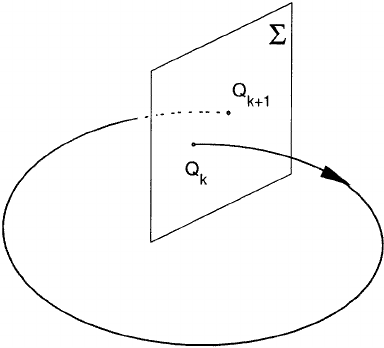
\includegraphics[width=0.5\textwidth]{PoincareMapSketch.png}
	\caption[Sketch of Poincar\'e map]{Sketch of the Poincar\'e map, taken from \cite{Abdullaev}.\label{PoincareMapSketch}}
\end{figure}

We end this section on a note about bifurcations. As mentioned at the beginning of this section, the first step studying the qualitative behaviour of systems of ODEs is to find equilibrium point(s) and study their local stability. This is done via constructing the Jacobian matrix of the system evaluated at an equilibrium point, and computing the eigenvalues of the matrix. We then classify local stability of the equilibrium point as follows:

\begin{prop}
	Let $x^*$ be an equilibrium point for the ODE
	$$\dot{x}=f(x)$$
	and let $DF(x^*)$ be the Jacobian matrix of $f(x)$ evaluated at $x^*$.
	\begin{itemize}
		\item If the real parts of all the eigenvalues of $DF(x^*)$ are strictly negative, the equilibrium point is locally asymptotically stable.
		\item If at least one of the eigenvalues of $DF(x^*)$ has strictly positive real part, the equilibrium point is unstable.
	\end{itemize}
\label{PropLocalStability}
\end{prop}

When an eigenvalue has zero real part, this method of stability analysis does not tell us whether or not the equilibrium point is stable. It is therefore useful to introduce the following definition.

\begin{defn}
	Let $x^*$ be an equilibrium point for an $n$-dimensional differential equations $$\dot{x}=f(x),$$
	and let $\lambda_1,\ldots,\lambda_n$ be the eigenvalues of $DF(x^*)$. If the real part of $\lambda_i$ is non-zero for all $i$, then we say that $x^*$ is \emph{hyperbolic}.
	\label{DefHypFP}
\end{defn}

When a fixed point for an ODE $\dot{x}=f(x)$ is hyperbolic, we can invoke the Hartman-Grobman Theorem \cite{Chicone} and use the Jacobian of $f$ to accurately study dynamics of the ODE around the fixed point. This can be used to show that hyperbolic fixed points are either locally asymptotically stable or unstable. When the ODE contains parameters, the fixed points as well as their local stability may depend on these parameters. Therefore, we can expect that varying parameters will change the stability of a hyperbolic fixed point. When this occurs, we say the system undergoes a \textit{bifurcation}. Although there are many types of bifurcations, we describe three common types that appear throughout our work.\\

The first type is a \textit{transcritical bifurcation}. This occurs when a system has at least two distinct equilibrium points that exchange stability. For example, consider the system
\begin{equation}
	\dot{x}=x(r-x),
	\label{TCBifSys}
\end{equation}
where $r\in\R$ is a parameter. This system has equilibrium points $x^*_1=0$ and $x^*_2=r$. The Jacobian matrix associated to this system is
$$J(x)=r-2x.$$
Evaluating $J$ at the equilibrium points, we obtain $J(x^*_1)=r$ and $J(x^*_2)=-r$. Therefore,
\begin{itemize}
	\item if $r>0$, $x^*_1$ is unstable and $x^*_2$ is stable.
	\item if $r<0$, $x^*_1$ is stable and $x^*_2$ is unstable.
\end{itemize}
We then observe a transcritical bifurcation at $r=0$. A bifurcation diagram is given in Figure \ref{BifTC}. Generally, this type of bifurcation occurs when the eigenvalue of an equilibrium point passes through zero.\\

\begin{figure}[h!]
	\centering
	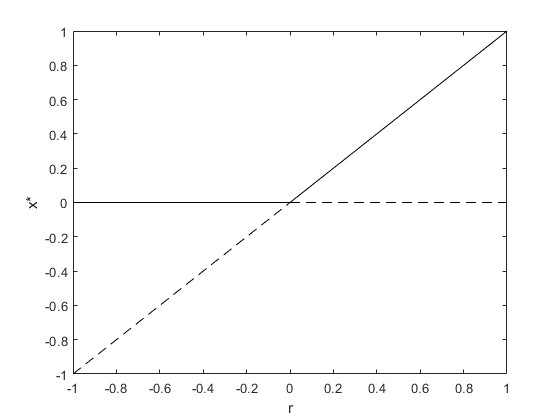
\includegraphics[width=0.5\textwidth]{BifTC.png}
	\caption[Trans-critical bifurcation]{Transcritical bifurcation in (\ref{TCBifSys}) at $a=0$. Steady states represented by a solid line are stable, and those by a dashed line are unstable.\label{BifTC}}
\end{figure}

The second type of bifurcation we present is a \textit{saddle-node} bifurcation. This occurs when a system has two distinct equilibrium points which collide and simultaneously vanish. For example, consider the system
\begin{equation}
	\dot{x}=a+x^2,
	\label{SNBifSys}
\end{equation}
where $a\in\R$ is a parameter. This system has equilibrium points $x^*_1=\sqrt{-a}$ and $x^*_2=-\sqrt{-a}$. Therefore, when $a<0$, there are two distinct equilibrium points. When $a=0$, we have that $x^*_1=x^*_2$, and once $a$ becomes positive, there are no equilibrium points. Moreover, the Jacobian is given by $J(x)=2x$, so if the equilibrium points exist, $x^*_1$ is unstable and $x^*_2$ is stable. A bifurcation diagram is given in figure \ref{BifSN}.\\

\begin{figure}[h!]
	\centering
	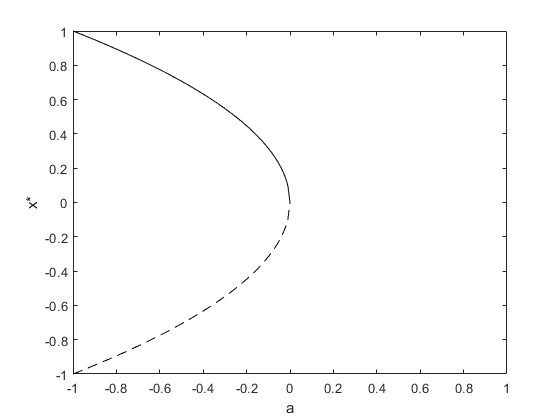
\includegraphics[width=0.5\textwidth]{BifSN.png}
	\caption[Saddle-node bifurcation]{Saddle-node bifurcation in (\ref{SNBifSys}) at $a=0$. Steady states represented by a solid line are stable, and those by a dashed line are unstable.\label{BifSN}}
\end{figure}

The third type of bifurcation we encounter in this work is a \textit{Hopf bifurcation}. This occurs when an equilibrium point undergoes a change in local stability and a periodic orbit emerges. We have the following theorem \cite{HaleKucak}.

\begin{theo}[Poincar\'e--Andronov--Hopf]
	Let $\dot{x}=A(\lambda)x+F(\lambda,x)$ be a three-times continuously differentiable planar vector field depending on a scalar parameter $\lambda$ such that $F(\lambda,0)=0$ and $D_xF(\lambda,0)=0$ for all sufficiently small $|\lambda|$. Assume that the linear part $A(\lambda)$ at the origin has the eigenvalues $\alpha(\lambda)\pm i\beta(\lambda)$ with $\alpha(0)=0$ and $\beta(0)\ne 0$. Furthermore, suppose that the eigenvalues cross the imaginary axis with nonzero speed; that is,
	$$\frac{d\alpha}{d\lambda}(0)\ne 0.$$
	Then, in any neighbourhood $U$ of the origin in $\R^2$ and any given $\lambda_0>0$, there is a $\bar{\lambda}$ with $|\bar{\lambda}|<\lambda_0$ such that the differential equation $\dot{x}=A(\bar{\lambda})x+F(\bar{\lambda},x)$ has a nontrivial periodic orbit in $U$, with period near $2\pi/\beta(0)$.
	\label{TheoHopfBIf}
\end{theo}

For example, consider the following model in polar coordinates

\begin{equation}
	\begin{split}
		\dot{r}&=(\lambda-ar^2)r,\\
		\dot{\theta}&=1+br^2,
	\end{split}
	\label{VicHopfEg}
\end{equation}
where $\lambda,a$ and $b$ are real positive parameters. A (non-trivial) periodic solution in this system corresponds to a positive steady state of the radial equation and a monotone solution of the angular equation. Since the right-hand side of the angular equation is strictly positive, any solution $\theta(t)$ will be monotone increasing. Moreover, a steady state of the radial equation can be found by solving
$$(\lambda-ar^2)r=0.$$
There are solutions $r^*=0$ and $r^*=\sqrt{\lambda/a}$, since we do not consider negative radii. The positive steady state is given by $\bar{r}=\sqrt{\lambda/a}$, under the condition that $\lambda/a>0$. Therefore, if we fix $a>0$, for example, and vary $\lambda$ through 0, a Hopf bifurcation will occur at $\lambda=0$ with limit cycles for $\lambda>0$. A bifurcation diagram of the radial equation is given in Figure \ref{BifH}, and we note that the periodic solution with $r^*=0$ can be thought of as the steady state at the origin.\\

\begin{figure}[h!]
	\centering
	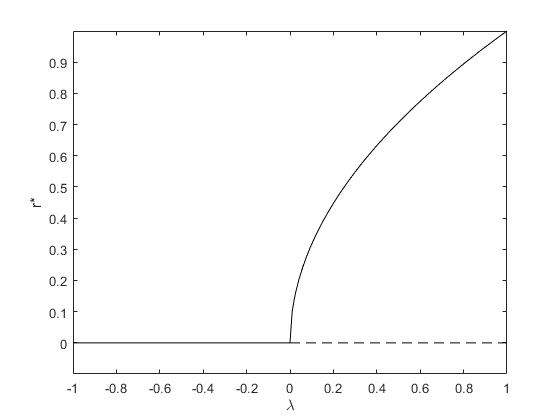
\includegraphics[width=0.5\textwidth]{BifH.png}
	\caption[Hopf bifurcation]{Hopf bifurcation in (\ref{VicHopfEg}) at $\lambda=0$. Curves give the radii of periodic solutions. Radii represented by a solid line indicate a stable periodic orbit, and those by a dashed line represent an unstable periodic orbit.\label{BifH}}
\end{figure}

\section{Floquet Theory}
\label{SectionFloquetTheory}
The method of finding the equilibrium points of a system and studying their local stability generally does not apply to non-autonomous systems, which we will encounter later. For example, if the function $f(t,x,\lambda)$ from (\ref{IVPDef}) depends explicitly on $t$, then it may be the case that there are no equilibrium points; i.e., no solutions of $f(t,x,\lambda)=0$ that are constant in $x$ and $\lambda$. As a result, we cannot consider local stability around a steady state, as they do not exist. However, the non-autonomous systems we encounter in this work are defined by time-periodic functions. These time-periodic systems typically have time-periodic solutions. To study their stability, we linearise and obtain a time-periodic linear equation. In particular, we have a linear system of the form
\begin{equation}
	\dot{x}=A(t)x,
	\label{FloqODE}
\end{equation}
where $x\in \R^n$ and $t\mapsto A(t)$ is a $T$-periodic continuous matrix-valued function. Section 2.4 of \cite{Chicone} details the study of these systems, known as Floquet theory. To state the main result, we first define a \textit{fundamental matrix solution} of (\ref{FloqODE}).

\begin{defn}
	A $n\times n$ matrix function $t\mapsto \Psi(t)$, defined on an open interval $J$, is called a \emph{matrix solution} of the homogeneous linear system (\ref{FloqODE}) if each of its columns is a (vector) solution. A matrix function is called a \emph{fundamental matrix solution} if its columns form a fundamental set of solutions; i.e., the columns form a basis for the space of solutions.
	\label{DefFundMatrixSoln}
\end{defn}

The main result of Floquet theory is as follows.

\begin{theo}[Floquet's Theorem]
	If $\Phi(t)$ is a fundamental matrix solution of the $T$-periodic system (\ref{FloqODE}), then, for all $t\in \R$,
	$$\Phi(t+T)=\Phi(t)\Phi^{-1}(0)\Phi(T).$$
	In addition, for each (possibly complex) matrix $B$ such that
	$$e^{TB}=\Phi^{-1}(0)\Phi(T),$$
	there is a (possibly complex) $T$-periodic matrix function $t\mapsto P(t)$ such that $\Phi(t)=P(t)e^{tB}$ for all $t\in \R$. Also, there is a real matrix $R$ and a real $2T$-periodic matrix function $t\mapsto Q(t)$ such that $\Phi(t)=Q(t)e^{tR}$ for all $t\in \R$.
	\label{TheoFloquetsTheorem}
\end{theo}
	
The representation $\Phi(t)=P(t)e^{tB}$ is the \textit{Floquet normal form}, which will be used to study the stability of the zero solution of periodic homogeneous linear systems. An important definition for the application of Floquet theory to this research is that of \textit{characteristic exponents}, $\mu$. These are defined as eigenvalues of the matrix $e^{TB}$. A similar notion is that of the \textit{characteristic multipliers}, defined by $\rho=e^{\mu T}$. It is important to note that the matrix $B$ from Floquet's Theorem, as well as the characteristic exponents, are not unique. This follows from the fact that the matrix exponential function is not injective; if $\mu$ is a characteristic exponent, then so is $\mu+2\pi ik/T$ for all $k\in\Z$. However, the characteristic eigenvalues are unique, and therefore the stability of the zero solution is uniquely determined.\\

Finally, we can use the characteristic multipliers/exponents to study stability of the zero solution of (\ref{FloqODE}). This is outlined in the following theorem.

\begin{theo}
	There is a time-dependent ($2T$-periodic) change of coordinates, $x=Q(t)y$, that transforms the periodic system (\ref{FloqODE}) to a (real) constant coefficient linear system.
	\begin{itemize}
		\item[(1)] If the characteristic multipliers of the periodic system (\ref{FloqODE}) all have modulus less than one --- equivalently, if all characteristic exponents have negative real part --- then the zero solution is asymptotically stable.
		
		\item[(2)] If any of characteristic multipliers of the periodic system (\ref{FloqODE}) have modulus greater than one --- equivalently, if any of the characteristic exponents have positive real part --- then the zero solution is unstable.
	\end{itemize}
	\label{TheoFloquetStability}
\end{theo}

The term \textit{Floquet multipliers} is used analogously when studying the Poincar\'e map of a periodic solution. With a choice of cross-section $\Sigma$ based at a point $x^*$ on the periodic solution, we can study the discrete-time dynamical system (defined locally around $x^*$) given by
\begin{flalign*}
Q\colon \Sigma&\rightarrow \Sigma,\\
 x&\mapsto Q(x).
\end{flalign*}
The stability of the periodic solution can be determined by the Floquet multipliers of the periodic solution, which are defined as the eigenvalues of $DQ(x^*)$. The stability of the periodic solution is then subject to Theorem \ref{TheoFloquetStability}, with ``periodic solution'' in place of ``zero solution''. We note in some scenarios that the Poincar\'e map is defined from an open ball around $x^*$ to itself. In this case, the eigenvalues will be the same Floquet multipliers are above, with an additional eigenvalue of 1. This eigenvalue corresponds to the eigenvector that is tangent to the periodic orbit ar $x^*$.\\

Although the above theory applies to $n$-dimensional systems of the form (\ref{FloqODE}), this thesis only goes as far as studying one-dimensional periodic homogeneous linear systems. We formally write these as
\begin{equation}
	\dot{x}=a(t)x,
	\label{FloqODE1D}
\end{equation}
where $x\in \R$ and $a\colon \R\rightarrow \R$ is a $T$-periodic function. In this case, we are able to explicitly calculate the characteristic multiplier/exponent.

\begin{theo}
	The characteristic exponents of (\ref{FloqODE1D}) are given by
	$$\mu=\frac{1}{T}\int_0^T a(s)\ ds+\frac{2\pi k i}{T}$$
	for any $k\in \Z$. Similarly, the characteristic multiplier of (\ref{FloqODE1D}) is given by
	$$\rho=e^{\int_0^T a(s)\ ds}.$$
	\label{TheoOneDimFLoquet}
\end{theo}
\begin{proof}
	We first solve the system (\ref{FloqODE1D}) explicitly, starting at $t=0$.
	\begin{flalign*}
		&\dot{x}=a(t)x\\
		\implies &\frac{\dot{x}}{x}=a(t)\\
		\implies &\ln \big|x(t)\big|=\int_{0}^t a(s)\ ds+\tilde{c}\\
		\implies &x(t)=ce^{\int_{0}^t a(s)\ ds}.
	\end{flalign*}
	If we suppose initial condition $x(0)=1$, then clearly $c=1$, so
	$$x(t)=e^{\int_{0}^t a(s)\ ds}.$$
	To find characteristic exponents, we first wish to find a matrix $B$ satisfying the condition
	\begin{equation}
		e^{TB}=\Phi(0)^{-1}\Phi(T),
		\label{FloqCond}
	\end{equation}
	where $\Phi(t)$ is a fundamental matrix solution, as per Floquet's Theorem. As we are in the one-dimensional case, $B$ is a number, and our above solution $x(t)=e^{\int_{0}^t a(s)\ ds}$ is a fundamental solution. Setting $\Phi(t)=x(t)$ in the condition (\ref{FloqCond}), we then obtain
	\begin{flalign*}
		e^{TB}&=\Phi(0)^{-1}\Phi(T)\\
		&=x(0)^{-1}x(T)\\
		&=x(T)\\
		&=e^{\int_{0}^T a(s)\ ds}.
	\end{flalign*}
	Taking the natural logarithm of both sides yields
	$$TB=\int_{0}^T a(s)\ ds+2\pi k i$$
	for $k\in \Z$.
	Therefore, we can take $B=\frac{1}{T}\int_{0}^T a(s)\ ds+\frac{2\pi k i}{T}$ for any $k\in\Z$. Since $B$ is a number, then if we consider it as a $1\times 1$ matrix, it is its own eigenvalue. Therefore, the characteristic exponents of (\ref{FloqODE1D}) are
	$$\mu=\frac{1}{T}\int_{0}^T a(s)\ ds+\frac{2\pi k i}{T}$$
	for any $k\in \Z$, and the characteristic multiplier is
	$$\rho=e^{\mu T}=e^{\int_{0}^T a(s)\ ds}.$$
\end{proof}
Using this theorem in conjunction with Theorem \ref{TheoFloquetStability}, we can take $k=0$ to tell us that
\begin{itemize}
	\item[(1)] if $\frac{1}{T}\int_{0}^T a(s)\ ds<0$, then the zero state of system (\ref{FloqODE1D}) is asymptotically stable.
	\item[(2)] if $\frac{1}{T}\int_{0}^T a(s)\ ds>0$, then the zero state of system (\ref{FloqODE1D}) is unstable.
\end{itemize}
If, by chance, we have $\frac{1}{T}\int_{0}^T a(s)\ ds=0$, the zero state is called \textit{Lyapunov stable}. In this work, however, we are not particularly interested in this case. We use Floquet theory to determine when a species can invade (see Section \ref{SectionInvAnalysis}), and therefore we only wish to satisfy statement (2) above.

\section{Averaging Differential Equations}
\label{SectionAvgDifEq}

Consider a non-autonomous ODE of the form
$$\dot{x}=A(t)x.$$
It may be the case that $A(t)$ is periodic in time, of period $T$, and variations in $A(t)$ are small. In particular, we may write
\begin{equation}
	\dot{x}=\epsilon \tilde{A}(t)x
	\label{AvgBabyEqn}
\end{equation}
for $\epsilon>0$ small. Although the ODE is still non-autonomous, the function $A(t)$ is \textit{almost} independent of time, in the sense that it only ever varies from its average by an order of $\epsilon$. It may seem intuitive then to study dynamics induced by the averaged system to approximate the dynamics of (\ref{AvgBabyEqn}). In this section, we detail this averaging process and discuss the applicability of this method.\\

In general, averaging is applicable to systems of the form
\begin{equation}
	\begin{split}
		\dot{x}=\epsilon f(x,t,\epsilon),
	\end{split}
	\label{AvgODE}
\end{equation}
where $x\in U\subseteq\R^n$, $0\le \epsilon \ll 1$, and $f\colon \R^n\times \R\times \R^+\rightarrow \R^n$ is $r$ times continuously differentiable, $r\ge 2$, bounded on bounded sets, and of period $T>0$ in $t$. We define the associated \textit{autonomous averaged system} as
\begin{equation}
	\dot{y}=\epsilon \bar{f}(y)\equiv\epsilon\frac{1}{T}\int_0^T f(y,t,0)dt.
	\label{AutAvgSys}
\end{equation}
We employ the following theorem, which is proved in \cite{GuckHolmes}.
\begin{theo}[The Averaging Theorem]
	There exists an $r$-times continuously differentiable change of coordinates $x=y+\epsilon w(y,t,\epsilon)$ under which (\ref{AvgODE}) becomes
	\begin{equation}
		\dot{y}=\epsilon \bar{f}(y)+\epsilon^2 f_1(y,t,\epsilon),
		\label{AvgPerSys}
	\end{equation}
	where $f_1$ is of period $T$ in $t$. Moreover,
	\begin{itemize}
		\item[(i)] If $x(t)$ and $y(t)$ are solutions of (\ref{AvgODE}) and (\ref{AutAvgSys}) based at $x_0,y_0$, respectively, at $t=0$, and $|x_0-y_0|=\mathcal{O}(\epsilon)$, then $|x(t)-y(t)|=\mathcal{O}(\epsilon)$ on a time scale $t=\mathcal{O}(1/\epsilon)$.
		\item[(ii)] If $p_0$ is a hyperbolic fixed point of (\ref{AutAvgSys}), then there exists $\epsilon_0>0$ such that, for all $0<\epsilon\le \epsilon_0$, (\ref{AvgODE}) possesses a unique hyperbolic periodic orbit $\gamma_\epsilon(t)=p_0+\mathcal{O}(\epsilon)$ of the same stability type as $p_0$. This periodic orbit may be trivial.
		\item[(iii)] If $x^s(t)\in W^s(\gamma_\epsilon)$ is a solution of (\ref{AvgODE}) lying in the stable manifold of the hyperbolic periodic orbit $\gamma_\epsilon=p_0+\mathcal{O}(\epsilon)$, $y^s(t)\in W^s(p_0)$ is a solution of (\ref{AutAvgSys}) lying in the stable manifold of the hyperbolic fixed point $p_0$ and $|x^s(0)-y^s(0)|=\mathcal{O}(\epsilon)$, then $|x^s(t)-y^s(t)|=\mathcal{O}(\epsilon)$ for $t\in[0,\infty)$. Similar results apply to solutions lying in the unstable manifolds on the time interval $t\in (-\infty,0]$.
	\end{itemize}
\label{TheoAveraging}
\end{theo}

We note that conclusions $(ii)$ and $(iii)$ generalize to more complicated hyperbolic sets: for example, if (\ref{AutAvgSys}) has a hyperbolic closed orbit, then (\ref{AvgODE}) has a corresponding hyperbolic invariant torus \cite{Hale}. Theorem (\ref{TheoAveraging}) allows us to study the averaged system associated to our non-autonomous seasonal model, and use our results to understand the behaviour of the seasonal model. In particular, we will look for steady states and periodic orbits in the averaged system and study their local stability. This translates directly to periodic orbits and invariant tori in of the seasonal model with the same stability type.\\

We will also be interested in bifurcations of our non-autonomous focal model. Consider a family of systems of the form
\begin{equation}
	\dot{x}=\epsilon f_\mu (x,t,\epsilon),
	\label{AvgBifODE}
\end{equation}
where $\mu\in \R$,  as well as the associated family of averaged systems
\begin{equation}
	\dot{y}=\epsilon \bar{f}_\mu (y).
	\label{AvgBifPerSys}
\end{equation}

There is a corresponding bifurcation theorem for averaged systems, whose proof can also be found in \cite{GuckHolmes}.

\begin{theo}
	If (\ref{AvgBifPerSys}) undergoes a saddle-node or a Hopf bifurcation at $\mu=\mu_0$, then, for $\mu$ near $\mu_0$ and $\epsilon$ sufficiently small, the Poincar\'e map of (\ref{AvgBifODE}) also undergoes a saddle-node or a Hopf bifurcation.
	\label{TheoAvgBif}
\end{theo}

\section{Predator--Prey Models}
\label{SectionPredPreyModels}

This thesis focuses on differential equations that model population dynamics and predator-prey interactions. Therefore, we discuss the relevant ecological phenomena and how they may be translated into differential equations. All of the material in this section can be found in \cite{Kot}.\\

The first step is understanding growth and death mechanisms of populations. We can then choose functions that take into account the key mechanisms that we would like to model and use these functions to derive our differential equations. To give a basic example, let $x=x(t)$ represent the population density of a species, and consider the following equation:
\begin{equation}
	\dot{x}=rx-mx.
	\label{PPLinear}
\end{equation}
The parameters $r,m\ge 0$ are per capita birth and death rates of the species. However, we can also define $a=r-m$ and write (\ref{PPLinear}) as
\begin{equation}
	\dot{x}=ax.
	\label{PPLinearCombine}
\end{equation}
In this case, we no longer have separate terms on the right-hand side of the equation, but rather a single term that encompasses all of the growth and death mechanisms that apply to the species. Throughout many ecological models, certain terms are commonly used to model population dynamics of a species. We list two important terms here.\\

\noindent{Exponential growth:}
\begin{equation}
	\dot{x}=ax.
	\label{ExponentialGrowth}
\end{equation}
The example we gave above, (\ref{PPLinearCombine}), represents exponential growth of a population. It is called such because solutions to (\ref{ExponentialGrowth}) are of the form
$$x(t)=ce^{at},$$
where $c$ is a constant that represents the initial condition. With the solution written as such, we can then see that, when $a>0$, the population increases indefinitely (given that we start with a non-zero population). This corresponds to the case where $r>m$ in equation (\ref{PPLinear}); in other words, the species growth outpaces its death. Similarly, if $a<0$, the population decreases to 0. Finally, if $a=0$, the population remains constant for all times.\\

\noindent{Logistic growth:}
\begin{equation}
	\dot{x}=rx\left(1-\frac{x}{K}\right).
	\label{LogisticGrowth}
\end{equation}
Logistic growth can be used to model a species that grows at low densities with growth rate $r$ but is limited by a carrying capacity $K$. When the population is above this carrying capacity, the rate of change is negative. Therefore, the population declines as it approaches the carrying capacity. We note that (\ref{LogisticGrowth}) is not written as a growth and death term separately. However, for $x<K$, $\dot{x}$ is positive, so the density increases; for $x>K$, the density decreases. Therefore, growth and death are taken into account via the carrying capacity.\\

In the case of predator--prey relationships, we will construct models that take into account multiple species and that will have growth and death terms that represent the interactions between the species. We can construct a general model for a prey, denoted by $x$, which has one predator, denoted by $y$. For example, we may write
\begin{equation}
	\begin{split}
		&\dot{x}=r(x)-m(x,y),\\
		&\dot{y}=cm(x,y)-u(y).
	\end{split}
	\label{GeneralPredPreyModel}
\end{equation}
In this setup, we define $r(x)$ as the net prey growth in the absence of the predator. $m(x,y)$ and $u(y)$ are taken to be non-negative functions. The term $m(x,y)$ represents predation-induced death of the prey, and $u(y)$ is predator death. Finally, $c$ represents the conversion coefficient of predation, which measures how a predator may convert prey consumption into its own population growth.

A classic example of a predator--prey model is the \textit{Lotka--Volterra} model \cite{Lotka}, given as
\begin{equation}
	\begin{split}
		&\dot{x}=ax-bxy,\\
		&\dot{y}=cxy-dy.
	\end{split}
	\label{LotkaVolterra}
\end{equation}
It can be shown that there is a unique steady state, which is stable but not asymptotically stable, given by
$$(x^*,y^*)=\left(\frac{d}{c},\frac{a}{b}\right).$$
All other positive solutions are periodic around this steady state \cite{Kot}.\\

Another famous, and slightly more complicated, predator--prey model is the \textit{Rosenzweig--MacArthur} model \cite{Kot, RosMac}. It reads
\begin{equation}
	\begin{split}
		&\dot{x}=rx\left(1-\frac{x}{K}\right)-\frac{mxy}{a+x},\\
		&\dot{y}=\frac{gxy}{a+x}-uy.
	\end{split}
	\label{RosMac}
\end{equation}

We will study the details of this model in Section \ref{SectionSimpOwl}. This system always has a trivial and prey-only state. In addition, the system may have a coexistence state. Moreover, the coexistence state may lose stability via a Hopf bifurcation, which gives rise to stable limit cycles in the system.\\

Throughout this work, we will create differential equations that model the interactions of a single prey with two distinct predators. We will use particular functions to describe growth and death terms of these species, as well as the predation of the predators on the prey.


\section{Functional Responses}
\label{SectionFunRes}

In the previous section, we introduced some possible forms of the function $r(x)$, which represents the net growth of the prey species. In this section, we will present some options for the function $m(x,y)$, which is a non-negative function representing prey death due to the predator.\\

We introduce the notion of a \textit{functional response} to motivate the choice of function $m(x,y)$. This is a term used in ecology to describe the way in which a prey responds to a predator; i.e., how many prey are killed per predator. Once enough field data is collected to understand the functional response, one can construct functions that fit the data and encompass the observed behaviour of the response. When a suitable functional response is found, which we denote by $\phi(x)$, where $x$ is the prey density, we can define the prey death term as
$$m(x,y)=\phi(x)y,$$
where $y$ is the predator density. Throughout this work, we will use the functional responses presented by C.S. Holling \cite{Holling1,Holling2}, as well as a third response \cite{Real}.\\

A type I functional response assumes a linear death rate with respect to prey density $x$, which is capped at some density $x^*$. Therefore, an appropriate choice of function is
\begin{equation}
	\phi_1(x)=\begin{cases}
		mx&\text{if }x\le x^*\\
		mx^*&\text{if }x\ge x^*
	\end{cases}
	\label{TypeIFR}
\end{equation}
where $m>0$ is a parameter.\\

A type II functional response assumes an approximately linear predation rate at low prey density, which tapers off to some maximal intake rate at higher prey density. The main difference between type I and II is that type I has a `corner' at $x^*$ whereas type II does not. An example of a function that exhibits this behaviour is \textit{Holling's disc equation} \cite{Holling2}, given by
\begin{equation}
	\phi_{2}(x)=\frac{mx}{a+x},
	\label{TypeIIFR}
\end{equation}
where $m,a>0$ are parameters. In fact, this function was mechanistically derived via an artificial predator--prey situation wherein a blindfolded subject `hunted' for discs on a table. The motivates the name \textit{disc equation}. The denominator in this functional response imposes the upper bound on intake rate as prey density is large. However, for small prey density, the type II functional response is approximated by the linear function $\frac{m}{a}x$. Moreover, $\phi_{2}(x)$ is monotone increasing and
$$\lim_{x\rightarrow\infty}\frac{mx}{a+x}=m,$$
which shows that this functional response is bounded above by $m$. We will refer to the parameter $m$ as the \textit{saturation killing rate}. Moreover, the parameter $a$ is the half-saturation constant; i.e., when $x=a$, the density is at half of its maximum capacity. Specialist predators typically show a functional response consistent with that of a type II. We note that function (\ref{TypeIFR}) also satisfies the desired behaviour of the type II functional response. In particular, this function is linear for low prey density and is bounded above when prey density is larger. The preference of a function such as (\ref{TypeIIFR}) is the continuous derivative for all positive values of prey density.\\

A type III functional response is also bounded above, but the behaviour at low densities differs from that of type I or type II. A type III response assumes a predation rate that is very low at low prey density, relative to the type I or II responses. The idea is that at low prey density, the predator does not encounter many of the focal prey items and hence will not bother to learn how to hunt them well. Alternatively, a predator may switch to alternative food sources at low focal prey density. In this case, the model must include an additional predator growth term, which represents the growth due to additional food sources. This term will not depend on prey density, and therefore this case will not fit into the framework of (\ref{GeneralPredPreyModel}). An example of an appropriate function is
\begin{equation}
	\phi_3(x)=\frac{mx^2}{a+x^2},
	\label{TypeIIIFR}
\end{equation}
where $m,a>0$ are constant parameters. $m$ can be again thought of as the saturation killing rate, and $a$ is the square of the half-saturation constant. The role of the denominator in this function is to impose an upper bound on prey consumption, similar to the type II functional response. However, as prey density decreases, this function is approximated by the quadratic function $\frac{m}{a}x^2$ and is therefore small when prey density is low. Moreover, type III has an inflection point, as opposed to types I and II. Therefore, there is a qualitative difference between type II and type III responses in that when $x$ is small, $\phi_2(x)$ is approximately linear whereas $\phi_3(x)$ is approximately quadratic. Moreover, a type II response typically has an inflection point, whereas a type II does not. Generalist predators typically show a functional response consistent with that of a type III. Figure \ref{HollingsTypes} compares functional responses of types I, II and III.\\

\begin{figure}[h]
	\centering
	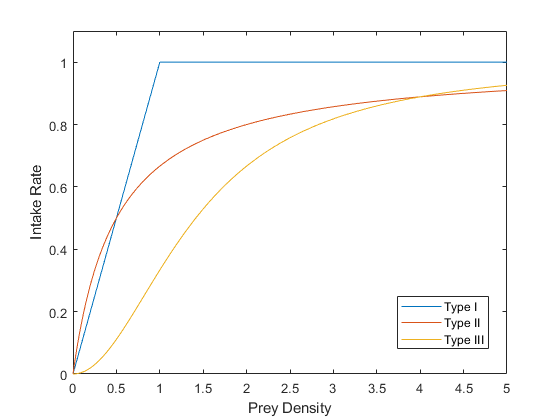
\includegraphics[width=0.5\textwidth]{HollingsTypes.png}
	\caption[Holling type functional responses]{Holling type functional responses. Type I: $ m=1$. Type II: $m=1,\ a=0.5$. Type III: $m=1,\ a=2$.\label{HollingsTypes}}
\end{figure}

Using these functional responses, we can now define suitable functions $m(x,y)$ for modelling predator--prey interactions. Throughout this work, these functions will be of the form
	$$m(x,y)=\phi_i(x)y$$
where the choice of functional response $\phi_i$ depends on the behaviour of the predator. The Canadian lynx is a specialist predator year round, which calls for a type II functional response. In addition to the preference of a continuous derivative, we choose the type II response for the lynx because empirical data predicts such a choice of functional response \cite{VitenseEtAl}. The great-horned owl is a specialist in the winter and a generalist in the summer, so we will model owl predation with type II and III responses, respectively.

\section{Invasion Analysis}
\label{SectionInvAnalysis}

The final section in this chapter will detail an approach called \textit{invasion analysis}, which we use to study some qualitative aspects of the complicated models encountered later in the work. Suppose we have a system with $n\ge 2$ species. One of the species is removed to obtain a system with $n-1$ species. We determine when this smaller system exhibits stable coexistence and derive conditions under which the missing predator can invade; i.e., grow at low density, at this coexistence state; we call these \textit{invasion conditions} for the removed species. In particular, we will define successful invasion  as this coexistence state being unstable in the direction of the missing species. This process is then repeated for all the species in the original system. Once the various invasion conditions are obtained, we check whether they can be satisfied simultaneously. If so, we are in the case of \textit{mutual invasion} in the $n$ species model. Finally, we aim to show that mutual invasion implies coexistence in the $n$ species model as well.\\

This process translates to studying local stability of semi-trivial states in an $n$-dimensional systems of ODEs; these are the steady states or periodic solutions where at least one component is zero. We provide an example to demonstrate the invasion analysis approach, and highlight its advantages and drawbacks.\\

Consider the following system with one predator and one prey, where $x$ is prey density and $y$ is predator density.
\begin{equation}
	\begin{split}
		\dot{x}&=rx(1-x)-mxy,\\
		\dot{y}&=gxy-uy.
	\end{split}
	\label{InvAnSys}
\end{equation}
$r,\ m,\ g$ and $u$ are taken to be strictly positive parameters. For the purpose of this work, we are interested in predator invasion. We know that, in the absence of the predator in (\ref{InvAnSys}), the prey exhibits logistic growth and therefore exists at a positive stable steady state. We wish to determine the predator invasion conditions at this steady state. In more detail, we first set the predator density to zero in the equations to obtain
\begin{flalign*}
	\dot{x}&=rx(1-x),\\
	\dot{y}&=0.
\end{flalign*}
We can consider the first equation as a 1-dimensional ODE, which has steady states $x^*=0$ and $x^*=1$. The positive state $x^*=1$ is always stable within the $x$-line, and corresponds to a semi-trivial state $(x^*,y^*)=(1,0)$ in (\ref{InvAnSys}). We then compute the Jacobian of (\ref{InvAnSys}), which, evaluated at the semi-trivial state, gives us
$$J(1,0)=\begin{bmatrix}
	-r & -m\\
	0 & g-u
\end{bmatrix}.$$
If we then consider the linearised system
\begin{flalign*}
	\begin{bmatrix}
		\dot{x} \\ \dot{y}
	\end{bmatrix}=\begin{bmatrix}
	-r & -m\\
	0 & g-u
\end{bmatrix}\begin{bmatrix}
x \\ y
\end{bmatrix},
\end{flalign*}
the predator equation decouples as
$$\dot{y}=(g-u)y.$$
We see that the state $(1,0)$ is unstable in the $y$ direction if $g-u>0$. Therefore when $g-u>0$, there will be a small region around $(1,0)$ in which solutions will diverge from $(1,0)$ along the $y$ direction. This means that if the predator invades the prey system with low density, it will initially increase in density. We consider this a successful invasion and so we take $g-u>0$ as the invasion condition for the predator.\\

We now verify that, under this invasion condition, we obtain coexistence in (\ref{InvAnSys}). The steady state of this system is given by
$$(x^*,y^*)=\left(\frac{u}{g},\frac{r}{m}\left(1-\frac{u}{g}\right)\right).$$
We note that this state is positive only if $1-\frac{u}{g}>0$ or $g-u>0$, which is the predator's invasion condition. The Jacobian of (\ref{InvAnSys}) evaluated at this steady state is
$$J(x^*,y^*)=\begin{bmatrix}
	-\frac{ru}{g} & -\frac{mu}{g}\\
	\frac{r}{m}\left(g-u\right) & 0
\end{bmatrix},$$
with characteristic polynomial
$$\lambda^2+\frac{ru}{g}\lambda+\frac{ru}{g}(g-u).$$
Since the parameters are assumed to be strictly positive, then, under the invasion condition, all of the coefficients in the characteristic polynomial are strictly positive. By the Routh--Hurwitz criterion \cite{Kot}, the roots of this polynomial will all have negative real parts. Therefore, the positive steady state is stable. We then see that if the predator can successfully invade in (\ref{InvAnSys}), then stable coexistence is achieved.\\

This example highlights the usefulness of the invasion analysis approach in that we can obtain conditions for stable coexistence in a two-dimensional system by studying the dynamics of various one-dimensional systems. Although general stability analysis is feasible in this case, it will be significantly harder in the three-species model that we encounter in this thesis. The main question we will ask ourselves then is whether or not mutual invasion implies stable coexistence in the three-species model. We can develop a sufficient understanding of the dynamics of the underlying two-species models, and invasion conditions of the third species are easy to write down. Therefore, if mutual invasion implies stable coexistence, these invasion conditions will also serve as sufficient conditions for coexistence. In some cases, mutual invasion and stable coexistence do not coincide, but we will spend some time investigating and discussing the relationship between these two. We end with the remark that species invasion at a steady state has often been studied, sometimes under the guise of \textit{persistence} \cite{DriesscheZeeman, LiSmith, XiaoFussman}. However, the scenario of invasion along a periodic orbit is not as common but is handled nicely by Floquet theory.

\cleardoublepage





\chapter{The Model}
\label{ChapterHLOChap6}

With much of the essential background theory laid out, we can formulate the ODE model with which we will study the dynamics of the snowshoe hare, Canadian lynx and great-horned owl. We first review the ecological literature in order to determine predation patterns of the lynx and the owl, as well as other growth and death mechanisms that affect all of our species. Once that is done, we translate these patterns and mechanisms into explicit functions that serve as the building blocks of our ODE model. We create one set of equations for the warmer portion of the year, which we refer to as the summer season from now on, and another set for the colder portion, which we call the winter season. Finally, we non-dimensionalize the model and take a functional average of the seasonal equations to remove the explicit time dependence of the system. The resulting model will be the focus of the remainder of this thesis. Our derivation closely follows the derivation of the model in \cite{TysonLutscher}. We generalize their approach by including the lynx that is the dominant predator of the snowshoe hare.\\

To formulate the model, we define a function $N=N(t)$ to represent the population of the hare over time. Similarly, we define $P=P(t)$ as the population of the lynx and $Q=Q(t)$ as the population of the owl. As we are considering a seasonal model, we also define $0<T< 1$ as the fraction of the year representing the summer season. During the summer, the hare grows logistically and is subject to predation by the lynx, a specialist predator, and the owl, a generalist. The lynx grows due to the consumption of the hare, and dies linearly. Finally, the owl grows in a logistic-like fashion, independent of the hare, in addition to growth due to the consumption of the hare. However, if the hares are not abundant, there is very little growth due to hare consumption. Using the functional forms of Section \ref{SectionFunRes}, the summer equations are given as
\begin{equation}
\begin{split}
&\frac{dN}{dt}=rN\left(1-\frac{N}{K}\right)-\frac{cNP}{b+N}-\frac{aN^2Q}{B^2+N^2},\\
&\frac{dP}{dt}=f\frac{cNP}{b+N}-mP,\\
&\frac{dQ}{dt}=h\frac{aN^2Q}{B^2+N^2}+\frac{sQ}{1+vQ}-uQ.
\end{split}
\label{SumEqns}
\end{equation}

During the winter season, hare growth is negligible due to insufficient resources, but predation due to both predators remains the leading cause of death. The lynx continues to act as a specialist predator with linear death rate. However, the owl acts as a specialist predator during this season due the unavailability of alternative prey, and continues to die linearly. Using the functional forms of Section \ref{SectionFunRes}, the winter equations read as
\begin{equation}
\begin{split}
&\frac{dN}{dt}=-\frac{cNP}{b+N}-\frac{\alpha NQ}{\beta+N},\\
&\frac{dP}{dt}=f\frac{cNP}{b+N}-mP,\\
&\frac{dQ}{dt}=h\frac{\alpha NQ}{\beta+N}-uQ.
\end{split}
\label{WinEqns}
\end{equation}

Interpretations of the parameters in (\ref{SumEqns}) and (\ref{WinEqns}) are given in Table \ref{TableHLOParameters}. We assume all parameters are strictly positive.\\

\begin{table}[h!]
	\centering
	\begin{tabular}{c | c | c}
		Parameter & Description & Units\\
		\hline
		$r$ & hare growth rate & 1/year\\
		$K$ & hare carrying capacity & hare\\
		$c$ & lynx saturation killing rate & hare/lynx/year\\
		$b$ & lynx half-saturation constant & hare\\
		$a$ & owl saturation killing rate (summer)  & hare/owl/year\\
		$B$ & owl half-saturation constant (summer) & $(\text{hare})^2$\\
		$f$ & lynx conversion efficiency & lynx/hare\\
		$m$ & lynx death rate & 1/year\\
		$h$ & owl conversion efficiency (summer)& owl/hare\\
		$s$ & owl alternative killing rate & 1/year\\
		$v$ & owl alternative density-dependence & 1/owl\\
		$u$ & owl death rate & 1/year\\
		$\alpha$ & owl saturation killing rate (winter) & hare/owl/year\\
		$\beta$ & owl half-saturation constant (winter) & hare
	\end{tabular}
\caption[Parameters in the seasonal model]{Parameters in (\ref{SumEqns}) and (\ref{WinEqns}).\label{TableHLOParameters}}
\end{table}


To formulate the complete seasonal model, we alternate between equation (\ref{SumEqns}) and (\ref{WinEqns}) according to season. We choose one year as our unit of time and start our year during the summer season. Thus, the summer equations (\ref{SumEqns}) are valid for $n\le t< n+T$ where $n$ is a non-negative integer, while the winter equations (\ref{WinEqns}) are valid for $n+T\le t< n+1$. We assume that the switch between seasons is instantaneous and population densities remain continuous, as the densities at the end of a season will serve as initial densities for the next season. Our seasonal model will then read
\begin{equation}
\begin{split}
&\underline{\text{Summer}:}\ t\in [n,n+T),\ n\in \Z\\
&\frac{dN}{dt}=rN\left(1-\frac{N}{K}\right)-\frac{cNP}{b+N}-\frac{aN^2Q}{B^2+N^2},\\
&\frac{dP}{dt}=f\frac{cNP}{b+N}-mP,\\
&\frac{dQ}{dt}=h\frac{aN^2Q}{B^2+N^2}+\frac{sQ}{1+vQ}-uQ,
\end{split}
\hspace{0.5in}
\begin{split}
&\underline{\text{Winter}:}\ t\in [n+T,n+1),\ n\in \Z\\
&\frac{dN}{dt}=-\frac{cNP}{b+N}-\frac{\alpha NQ}{\beta+N}\\
&\frac{dP}{dt}=f\frac{cNP}{b+N}-mP,\\
&\frac{dQ}{dt}=h\frac{\alpha NQ}{\beta+N}-uQ.
\end{split}
\label{SeasonalModel}
\end{equation}

To simplify the analysis, we non-dimensionalize the model. This will help identify important parameter combinations as well as reduce the overall number of parameters in the system. We define the following new quantities:
\begin{equation*}
	\begin{split}
		&x=\frac{N}{K},\\
		&y=\frac{cP}{rK},\\
		&z=\frac{aQ}{rK},\\
		&\tau=rt,\\
		&\overline{b}=\frac{b}{K},
	\end{split}
	\hspace{0.5in}
	\begin{split}
		&\overline{B}=\frac{B^2}{K^2},\\
		&\overline{a}=\frac{\alpha}{a},\\
		&d=\frac{\beta}{K},\\
		&\overline{f}=\frac{fc}{rK},\\
		&\overline{m}=\frac{m}{r},
	\end{split}
	\hspace{0.5in}
	\begin{split}
		&\overline{h}=\frac{ha}{r},\\
		&g=\frac{h\alpha}{r},\\
		&\overline{s}=\frac{sa}{r^2K},\\
		&\overline{v}=\frac{a}{vKr},\\
		&\overline{u}=\frac{u}{R}.
	\end{split}
\end{equation*}
Substituting these new quantities into (\ref{SeasonalModel}) and dropping the overhead bars, defining the overhead dot as the derivative with respect to $\tau$, we obtain
\begin{equation}
	\begin{split}
		&\underline{\text{Summer}}\ t\in [n,n+T),\ n\in \Z\\
		&\dot{x}=x(1-x)-\frac{xy}{b+x}-\frac{x^2 z}{B+x^2},\\
		&\dot{y}=\frac{fxy}{b+x}-my,\\
		&\dot{z}=\frac{hx^2z}{B+x^2}+\frac{sz}{v+z}-uz,
		\end{split}
		\hspace{0.5in}
		\begin{split}
		&\underline{\text{Winter}}\ t\in [n+T,n+1),\ n\in \Z\\
		&\dot{x}=\frac{xy}{b+x}-\frac{axz}{d+x},\\
		&\dot{y}=\frac{fxy}{b+x}-my,\\
		&\dot{z}=\frac{gxz}{d+x}-uz.
	\end{split}
	\label{NonDimSeasonalModel}
\end{equation}
Finally, we wish to write (\ref{NonDimSeasonalModel}) as a single system of ODEs. To do so, we define a new function $S:\R\rightarrow \{0,1\}$ as
\begin{equation*}
	S(t)=\begin{cases}
		1, & \text{if } n\le t< n+T, n\in \Z\\
		0, & \text{if } n+T\le t<n+1, n\in \Z
	\end{cases}.
\end{equation*}
In other words, $S(t)$ is equal to 1 during the summer season and equal to 0 during the winter. We can then write the model as
\begin{equation}
	\begin{split}
		&\dot{x}=S(t)\left(x(1-x)-\frac{xy}{b+x}-\frac{x^2 z}{B+x^2}\right)+(1-S(t))\left(\frac{xy}{b+x}-\frac{axz}{d+x}\right),\\
		&\dot{y}=\frac{fxy}{b+x}-my,\\
		&\dot{z}=S(t)\left(\frac{hx^2z}{B+x^2}+\frac{sz}{v+z}-uz\right)+(1-S(t))\left(\frac{gxz}{d+x}-uz\right).
	\end{split}
	\label{NonDimSeasonalODE}
\end{equation}

The seasonal model (\ref{NonDimSeasonalODE}) is difficult to study. This is partly due to the discontinuity of $S(t)$, but mostly due to the fact that the system is not autonomous. To address this issue, we use temporal averaging to create a much simpler, autonomous model that still contains the biological mechanisms that influenced the creation of the seasonal model (\ref{NonDimSeasonalODE}). Guided by the theory in Section \ref{SectionAvgDifEq}, we take the functional average of (\ref{NonDimSeasonalODE}) over the length of one period, which is 1. A problem that we encounter with this approach is that system (\ref{NonDimSeasonalODE}) is not continuous, which is a requirement for Theorem \ref{TheoAveraging}, and moreover there is no obvious choice of a small parameter to take the role of $\epsilon$ in Theorem (\ref{TheoAveraging}). To circumvent the first issue, one can use bump functions to approximate (\ref{NonDimSeasonalODE}) to an arbitrary degree with infinitely differentiable functions. Details can be found in many textbooks on analysis and/or distributions; for example \cite{Grubb}. We still do not have a small parameter, however. There is no obvious choice for such a parameter in (\ref{NonDimSeasonalODE}); nevertheless, we adopt the averaging approach since it has been shown to give good approximations. For example, when $y=0$, Tyson \& Lutscher give several examples where averaged dynamics accurately predict seasonal dynamics \cite{TysonLutscher}. In \cite{HsuZhao}, Hsu \& Zhao study the period map of a seasonal-competition model, and the stability conditions they obtain agree identically with those of the averaged model. The averaged system corresponding to (\ref{NonDimSeasonalODE}) is then
\begin{equation}
\begin{split}
&\dot{x}=T\Big(x(1-x)-\frac{xy}{b+x}-\frac{x^2 z}{B+x^2}\Big)+(1-T)\Big(-\frac{xy}{b+x}-\frac{axz}{d+x}\Big),\\
&\dot{y}=\frac{fxy}{b+x}-my,\\
&\dot{z}=T\Big(\frac{hx^2z}{B+x^2}+\frac{sz}{v+z}-uz\Big)+(1-T)\Big(\frac{gxz}{d+x}-uz\Big).
\end{split}
\label{HLO}
\end{equation}

Descriptions and ranges of the parameters found in (\ref{HLO}) are given in Table \ref{TableHLONonDimParameters}. Once again, parameters are taken to be strictly positive.
\begin{table}[h!]
	\centering
	\begin{tabular}{c | C{5cm} | c | c | c}
		Parameter & Description & Units & Range & Reference\\
		\hline
		$b$ & Lynx half-saturation & hare/ha & 0.3--1.5 & \cite{RuggerioAubryBuskirkKoehlerKrebsMcKelveySquires}\\
		$B$ & Owl half-saturation constant (generalist)& $(\text{hare/ha})^2$ & 0.0049--0.09 & \cite{TysonLutscher}\\
		$a$ & Owl saturation killing rate (specialist) & hare/owl/year & 0.4--2.7 & \cite{TysonLutscher}\\
		$d$ & Owl half-saturation constant (specialist) & hare/ha & 0.004--0.6 & \cite{KrebsBoutinDoonstra}\\
		$f$ & Hare--lynx conversion efficiency & 1/year & 2.75--3.2 & \cite{VitenseEtAl,StrohmTyson}\\
		$m$ & Lynx death rate in absence of hare& 1/year & 2--2.4 & \cite{VitenseEtAl,StrohmTyson}\\
		$h$ & Hare--owl conversion efficiency (generalist)& 1/year & 0.33--1 & \cite{ArtusoHoustonSmithRohner,SmithMurphy}\\
		$s$ & Owl alternative killing rate (generalist) & owl/year & 1.4 & \cite{ArtusoHoustonSmithRohner,SmithMurphy}\\
		$v$ & Owl alternative density dependence (generalist) & owl/ha & unknown &\\
		$u$ & Owl death rate & 1/year & 0.07--0.9 & \cite{ArtusoHoustonSmithRohner,HoustonFrancis}\\
		$g$ & Hare--owl conversion efficiency (specialist) & 1/year & 0.33--1 & \cite{ArtusoHoustonSmithRohner,SmithMurphy}\\
	\end{tabular}
	\caption[Parameters in the averaged model, and their values]{Parameters in (\ref{HLO}), and their values.}
	\label{TableHLONonDimParameters}
\end{table}
\cleardoublepage

\chapter{Simplifications of the Model}
\label{ChapterSimpOfModel}

The non-dimensionalization process as well as the averaging technique serve to simplify the seasonal model (\ref{SeasonalModel}) significantly. In general, ODE analysis is much simpler for autonomous systems with a minimal amount of free parameters. However, the high degree of nonlinearity in the focal model (\ref{HLO}) results yet again in a complicated analysis. In this chapter, we present an alternative direction to study this model. We will formulate various simplifications, aiming to remove some of the nonlinear aspects of (\ref{HLO}) that introduce difficulties in the analysis. Moreover, we motivate our choices of simplifications; we aim to apply techniques previously used in the study of predator--prey systems to which a simpler model lends itself, but we also ensure that the simplified models we create remain biologically relevant to our predator--predator--prey scenario. The goal of these simplifications is to develop new approaches that we may apply to the focal model (\ref{HLO}), as well as notice trends in the simplified models that we can look for in the non-simplified case.

\section{Hare--Owl Submodel}
\label{SectionHOSubmodel}

We recall that in the invasion analysis approach that we hope to apply, it is necessary to understand the dynamics of the underlying two-species model. The hare--lynx model of (\ref{HLO}) is a Rosenzweig--MacArthur model for which we understand the dynamics. However, the hare--owl model is more complicated. This two-species model reads
\begin{equation}
	\begin{split}
		&\dot{x}=T\Big(x(1-x)-\frac{x^2 z}{B+x^2}\Big)+(1-T)\Big(-\frac{axz}{d+x}\Big),\\
		&\dot{z}=T\Big(\frac{hx^2z}{B+x^2}+\frac{sz}{v+z}-uz\Big)+(1-T)\Big(\frac{gxz}{d+x}-uz\Big).
	\end{split}
	\label{HO}
\end{equation}\\
The model has already been analysed. For example, the summer equations are studied in \cite{ErbachLutscherSeo}, and the full model in \cite{TysonLutscher}. This model has a wide range of possible dynamics, including bistability and limit cycles. Moreover, an analytic study of this model is very difficult, and the majority of the results in \cite{TysonLutscher} are purely numerical. As our focal model (\ref{HLO}) extends this model to include a second predator, the lynx, we wish to further the analysis of (\ref{HO}) in order to understand its role in the study of the focal model.\\

We wish to develop some analytical tools for studying this model. To do so, we introduce a simplification of (\ref{HO}) for which the growth and death mechanisms are similar, but the particular equations are much simpler to work with. We first replace the alternative growth of the owl, given by the term
$$\frac{sz}{v+z}-uz,$$
with logistic growth
$$sz(1-z).$$
These two terms are qualitatively similar as functions of $z$, as seen in Figure \ref{OwlLogVsAlt}. In particular, both growth functions have zeros at $z=0$ as well as some positive value of $z$, and we can choose parameters such that these positive values coincide at 1. Moreover, we can simultaneously ensure that the growth rates at $z=0$ are equal.
\begin{figure}[h!]
	\centering
	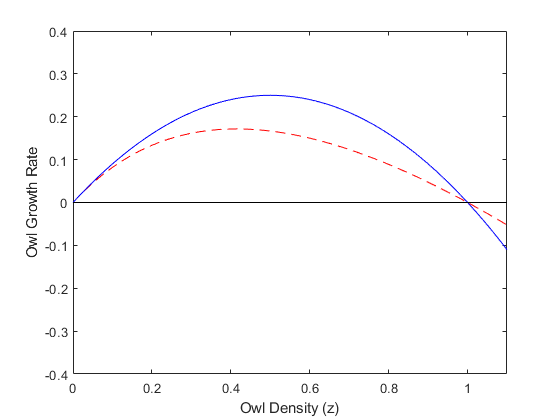
\includegraphics[width=0.7\textwidth]{OwlAltVsLogGrowth.png}
	\caption[Alternative growth and logistic growth for the owl]{Alternative growth (dashed red) and logistic growth (solid blue) functions for the owl. The solid black curve represents the $x$-axis. For alternative growth, $s=2$, $u=1$, $v=1$. For logistic growth, $s=1$.\label{OwlLogVsAlt}}
\end{figure}

We recall from Section \ref{SectionFunRes} that the specialist and generalist predation terms both include denominators, which serve to bound consumption by the predators at high prey density. In the case of the hare--owl system, the logistic growth forces an upper bound on prey density. Therefore, prey consumption must also be bounded above, as it depends strictly on the amount of prey available. This motivates the decision to remove the denominators, as we obtain much simpler polynomial equations while ensuring that a bounding mechanism for prey consumption is still present in the model.\\

Finally, we are left with a simplified hare--owl model, which reads
\begin{equation}
	\begin{split}
		&\dot{x}=T\Big(x(1-x)-Bx^2z\Big)+(1-T)\Big(-dxz\Big)=F(x,z),\\
		&\dot{z}=T\Big(hx^2z+sz(1-z)\Big)+(1-T)\Big(gxz-uz\Big)=G(x,z).
	\end{split}
	\label{HOsimp}
\end{equation}

For the summer-only case ($T=1$), this model is similar to work done by Magal et al \cite{MagalCosnerRuanCasas} where they study two logistically growing species and a Holling type II functional response. We can completely determine the dynamic behaviour of (\ref{HOsimp}) in the biologically relevant quadrant ($x\ge 0$ and $z\ge 0$). To do so, we consider the nontrivial hare and owl nullclines of the system, given, respectively, by

\begin{equation}
	z=N_h(x)=\frac{T(1-x)}{TBx+(1-T)d}
	\label{HOsimpHareNullcline}
\end{equation}
and
\begin{equation}
	z=N_o(x)=\frac{1}{Ts}\Big(T(hx^2+s)+(1-T)(gx-u)\Big).
	\label{HOsimpOwlNullcline}
\end{equation}\\

\begin{theo}
	If $N_h(0)>N_o(0)$ and $N_o(1)>0$, then the hare and owl nullclines, (\ref{HOsimpHareNullcline}) and (\ref{HOsimpOwlNullcline}) respectively, intersect exactly once in the positive quadrant of the $(x,z)$-plane. In this case, there exists a unique globally stable coexistence point of (\ref{HOsimp}).
	\label{TheoHOSimpCoex}
\end{theo}

\begin{proof}
We begin by finding a forward invariant domain for the system, by considering the nullclines. Setting $\tilde{x}=1+\epsilon$ for small $\epsilon>0$ and
$$\tilde{z}=\max\left\{\frac{1}{2}, N_o(\tilde{x})\right\},$$
we define the region
$$D=[0,\tilde{x}]\times[0,\tilde{z}].$$

\begin{figure}[h!]
	\centering
	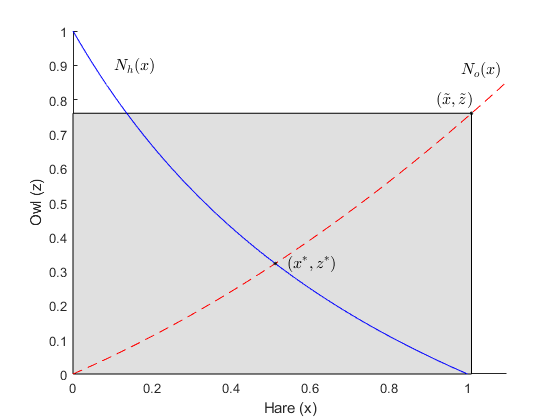
\includegraphics[width=0.8\textwidth]{HOSimpInvariantDomain.png}
	\caption[Invariant domain of the simplified hare--owl system]{$D$ is the greyed region above. The non-trivial hare (solid blue) and owl (dashed red) nullclines intersect in the interior of $D$ to give a coexistence point $(x^*,z^*)$. Parameters are $T=0.5$, $B=1$, $a=1$, $s=2$, $h=0.5$, $g=1$ and $u=2$.\label{HOSimpInvDom}}
\end{figure}

We define $\tilde{z}$ such that it is always strictly positive. We will show that $D$ is invariant with respect to the vector field (\ref{HOsimp}) by showing that the vector field is pointing inwards along the boundary $\partial D$. \\

As with all population models \cite{Kot}, the positive quadrant in the $x$-$z$ plane is invariant. Therefore, we must only look at the boundary segments along the lines $x=\tilde{x}$ and $z=\tilde{z}$. Consider the derivatives of the non-trivial nullclines,
$$N'_h(x)=\frac{-(1-T)d-T^2B}{(TBx+(1-T)d)^2}$$
and
$$N'_o(x)=\frac{2hs}{x}+\frac{(1-T)g}{Ts}.$$
Since $0<T<1$ and $x\ge 0$, we observe that $N_h(x)$ is monotone decreasing and $N_o(x)$ is monotone increasing.\\

Now, choose any point $(x,z)$ above the graph of $N_h(x)$. We have that
\begin{flalign*}
&z>\frac{T(1-x)}{TBx+(1-T)d}\\
\implies& \Big(TBx+(1-T)B\Big)z>T-Tx\\
\implies& 0 >T-Tx-\Big(TBx+(1-T)d\Big)z\\
&= T-Tx-TBxz-(1-T)dz\\
&=T\Big(1-x-dxz\Big)+(-T)\Big(-bz\Big).
\end{flalign*}
Multiplying through by $x\ge 0$, we obtain $0>F(x,z)$. Therefore, $\dot{x}<0$ above $N_h(x)$ and $\dot{x}>0$ below. Similarly, if we choose a point $(x,z)$ above the graph of $N_o(x)$, we can show that $G(x,z)<0$ so $\dot{z}<0$ above $N_o(x)$ and $\dot{z}>0$ below.\\

Now, consider the segment of $\partial D$ along the line $x=\tilde{x}$, which is given by
$$D_x=\{\tilde{x}\}\times (0,\tilde{z}].$$
Since $N_h(1)=0$ and $\tilde{x}>1$, we must have $N_h(\tilde{x})<0$ as $N_h$ is strictly decreasing. Therefore, $D_x$ lies completely above the graph of $N_h$, so $\dot{x}<0$ along $D_x$ and the vector field (\ref{HOsimp}) is pointing inwards along this segment.\\

Simarly, the segment of $\partial D$ along the line $z=\tilde{z}$ is given by
$$D_z=(0,\tilde{x})\times \{\tilde{z}\}.$$
As $N_o$ is increasing, it attains its maximum on $[0,\tilde{x}]$ at $x=\tilde{x}$. Therefore, $D_z$ lies above the graph of $N_o(x)$. Therefore, $\dot{z}<0$ along $D_z$ so the vector field is pointing inwards along $D_z$. We conclude that the region $D$ is an invariant domain for the flow of (\ref{HOsimp}).\\

The next step is to determine when a positive steady state exists in the interior of $D$. We first note that, since $N_h$ is strictly increasing and $N_o$ is strictly decreasing, these nontrivial nullclines can intersect at most once, so there is at most one positive steady state. The goal is now to determine under which conditions the nullclines intersect. Due to the monotonicity of $N_h$ and $N_o$, sufficient conditions can be given by
\begin{equation}
N_h(0)>N_o(0)
\label{HOIntCond1}
\end{equation}
and
\begin{equation}
N_o(1)>0.
\label{HOIntCond2}
\end{equation}
Since $N_h(1)=0$, the second condition implies $N_h(1)<N_o(1)$ and so, by the intermediate value theorem, we have $N_h(x^*)=N_o(x^*)$ for some $x^*\in (0,1)$. Therefore, the point $(x^*,z^*)=\Big(x^*,N_h(x^*)\Big)$ is the unique positive steady state.\\

Finally, we suppose conditions (\ref{HOIntCond1}) and (\ref{HOIntCond2}) are met so that the positive steady state $(x^*,z^*)$ exists. We wish to show that it is globally asymptotically stable. To do so, we define $D^o$ as the interior of $D$. In particular, $D^o=D\setminus \partial D.$
By a similar argument as above, $D^o$ is invariant with respect to the vector field (\ref{HOsimp}). We now define a function $\varphi(x,z)=\frac{1}{xz}$ and compute $\nabla(\varphi F,\varphi G).$ With
$$\frac{\partial \varphi F}{\partial x}=-\frac{T}{z}$$
and
$$\frac{\partial \varphi G}{\partial z}=-TB-\frac{Ts}{x},$$
we obtain
\begin{flalign*}
\nabla(\varphi F,\varphi G)=& \frac{\partial \varphi F}{\partial x}+\frac{\partial \varphi G}{\partial z}\\
=& -\frac{T}{z}-TB-\frac{Ts}{x}.
\end{flalign*}
It is then clear that $\nabla(\varphi F,\varphi G)<0$  for all $x,z>0$. In particular, we have $\nabla(\varphi F,\varphi G)<0$ in $D_\delta.$ By the Bendixson--Dulac criterion (Theorem \ref{TheoBendixsonDulac}), we conclude that there can be no periodic orbits in $D_\delta$. Furthermore, as $D_\delta$ is open and invariant with respect to the flow of (\ref{HOsimp}), the $\omega$-limit sets of any orbit must lie within $D_\delta.$ As there can be no periodic orbits and there is only one steady state in $D_\delta$, the Poincar\'e--Bendixson Theorem (Theorem \ref{TheoPoincareBendixson}) implies that the $\omega$-limit set of any orbit consists solely of the positive steady state. A steady state can only occur at the intersection of the hare and owl nullclines; therefore the unique intersection point of these nullclines in $D$ is the $\omega$-limit set of any orbit of (\ref{HOsimp}). In other words, the positive steady state $(x^*,z^*)$ must be stable if it exists.
\end{proof}

Although the theorem only gives a sufficient condition for stable coexistence at a steady state, we can argue that the only possible coexistence is at a stable steady state. First, we can argue diagrammatically, by looking at Figure \ref{HOSimpInvDom}, that the conditions in Theorem \ref{TheoHOSimpCoex} are in fact necessary. A steady state corresponds to an intersection of the blue and red curves, and if these curves are to cross, it is necessary that at $x=0$ and $x=1$ the conditions of Theorem \ref{TheoHOSimpCoex} are satisfied. Moreover, the use of the Bendixson--Dulac criterion in the proof of this theorem rules out any possibility of periodic solutions, so the only stable equilibrium we can have is the stable steady state in Figure \ref{HOSimpInvDom}.\\

This provides us with a sufficient understanding of the dynamics in the simplified hare--owl system (\ref{HOsimp}). We have explicit conditions for existence and stability of the positive steady state. We know from \cite{TysonLutscher} that the non-simplified hare--owl subsystem exhibits a wide array of complex dynamics, so we expect significant qualitative changes in dynamics as we move from the simplified three-species models to the original model (\ref{HLO}), but the results of this section serve as a good starting point to when we consider these simplified models.


\section{Simplfied Lynx \& Owl Model}
\label{SectionSimpLO}

In the previous section, removing the denominators of the hare--owl model  (\ref{HO}) allowed us to completely classify the population dynamics. Therefore we hope to simplify the focal model (\ref{HLO}) in the same way as we had for the hare--owl model (\ref{HO}), by omitting denominators in the equations and replacing the alternate growth of the owl by logistic growth. As such, this section will focus on the following model:
\begin{equation}
	\begin{split}
		&\dot{x}=T\Big(x(1-x)-b xy-B x^2z\Big)+(1-T)\Big(-b xy-d xz\Big),\\
		&\dot{y}=fxy-my,\\
		&\dot{z}=T\Big(hx^2z+sz(1-z)\Big)+(1-T)\Big(gxz-uz\Big).
	\end{split}
	\label{HLOsimp}
\end{equation}

The analysis of this model is not as straightforward as it was for the hare--owl model. Understanding the dynamics of the hare--owl model (\ref{HO}) relied on ODE theory for planar systems, such as the Bendixson--Dulac criterion and the Poincar\'e--Bendixson Theorem. Moreover, the arguments with nullclines do not translate well from a two-dimensional system to a three-dimensional system, as it is difficult to ensure intersections of three nullsurfaces simultaneously. Therefore, to study coexistence in (\ref{HLOsimp}), we must explicitly study stability of the various steady states of the system.\\

In the case of (\ref{HLOsimp}), we can have steady states with different combinations of species, such as hare only, owl only, hare-lynx, hare-owl, and all three. For example, the unique non-trivial steady state of the (\ref{HLOsimp}) is
\begin{equation}
	\begin{split}
		&x^*=\frac{m}{f},\\
		&y^*=\frac{1}{b}\Big(T\big(1-x^*-Bx^*z^*\big)+(1-T)\big(-dz^*\big)\Big),\\
		&z^*=\frac{1}{Ts}\Big(Th(x^*)^2+(1-T)gx^*+Ts-(1-T)u\Big).
	\end{split}
	\label{HLOsimpCoexPt}
\end{equation}
These equations are already complicated, and determining their stability will add another layer of complexity by having to calculate eigenvalues for matrices whose entries contain combinations of the steady-state expressions. It does not seem promising then to proceed with the study of stability at the nontrivial steady state. Instead, we apply the invasion analysis process to (\ref{HLOsimp}), as outlined in Section \ref{SectionInvAnalysis}.\\

We begin with the owl-invasion scenario. Following Section \ref{SectionInvAnalysis}, we first set $z=0$ in equations (\ref{HLOsimp}) to obtain the hare--lynx submodel. The resulting system is

\begin{equation}
	\begin{split}
		&\dot{x}=Tx(1-x)-b xy,\\
		&\dot{y}=fxy-my,\\
		&\dot{z}=0.
	\end{split}
	\label{HLOsimpz=0}
\end{equation}

The next step is to determine when the above system has a stable coexistence point. We first solve for the non-trivial steady state(s) $(x^*,y^*,0)$. From the $y$ equation, we must have
$$x^*=\frac{m}{f}.$$
We then solve for $y^*$ in the $x$ equation, giving us
\begin{equation*}
	y^*=\frac{T}{b}(1-x^*)=\frac{T}{b}\left(1-\frac{m}{f}\right).
\end{equation*}
This gives us the steady state 
\begin{equation}
	(x^*,y^*,0)=\left(\frac{m}{f}, \frac{T}{b}\left(1-\frac{m}{f}\right),0\right).
	\label{HLOsimpz=0SteadyState}
\end{equation}

It is clear that the steady state is biologically relevant if and only if $0<\frac{m}{f}<1$. We now wish to determine when it is stable in the $(x,y)$-plane. To do so, consider the Jacobian matrix
$$J(x,y,z)=\begin{bmatrix}
	T-2Tx -by & -bx & 0\\
	fy & fx-m & 0\\
	0 & 0 & 0
\end{bmatrix}.$$
Evaluating this matrix at the steady state (\ref{HLOsimpz=0SteadyState}) yields
\begin{equation*}
	\begin{split}
	J\left(\frac{m}{f}, \frac{T}{b}\left(1-\frac{m}{f}\right),0\right)&=\begin{bmatrix}
		T-2T\frac{m}{f} -b\frac{T}{b}\left(1-\frac{m}{f}\right) & -b\frac{m}{f} & 0\\
		f\frac{T}{b}\left(1-\frac{m}{f}\right) & f\frac{m}{f}-m & 0\\
		0 & 0 & 0
	\end{bmatrix}\\ \\
	&=\begin{bmatrix}
		-T\frac{m}{f} &  -\frac{bm}{f} & 0\\
		\frac{fT}{b}\left(1-\frac{m}{f}\right) & 0 & 0\\
		0 & 0 & 0
	\end{bmatrix}
	\end{split}.
\end{equation*}
This matrix is stable in the $(x,y)$-plane precisely when the eigenvalues of the top-left $2\times 2$ block, which we refer to as $J^*$, are both negative. Rather than calculating the eigenvalues explicitly, however, we know that the trace of $J^*$ will be the sum of the eigenvalues, and the determinant of $J^*$ will be the product of the eigenvalues. Moreover, the matrix $J^*$ has the sign pattern
$$\begin{bmatrix}
	- & -\\
	+ & 0
\end{bmatrix}.$$

The trace of $J^*$ is negative whereas the determinant is positive. If the product of both eigenvalues must be positive, then they must be of the same sign. Moreover, their sum is negative, so they must both be negative. We conclude that both eigenvalues are negative, and that the steady state (\ref{HLOsimpz=0SteadyState}) stable. To summarize, we have the following.

\begin{theo}
	Suppose $0<\frac{m}{f}<1$. Then there exists a unique positive steady state of the hare--lynx subsystem (\ref{HLOsimpz=0}), given by
	\begin{equation}
	\left(\frac{m}{f}, \frac{T}{b}\left(1-\frac{m}{f}\right),0\right),
	\label{HOSubStbCoexPt}
	\end{equation}
	and it is stable.
	\label{TheoremHLOSimpHLCoex}
\end{theo}

We note that this is a common theorem, and not original to this thesis. It can be found in many textbooks, for example \cite{Kot}.\\

The last step in the invasion analysis process is to determine under which conditions the owl can invade at this coexistence point. In other words, we derive conditions under which the state $z=0$ is unstable in the simplified model (\ref{HLOsimp}), given that $0<\frac{m}{f}<1$. To do so, we consider the Jacobian of the simplified system evaluated at the steady state (\ref{HOSubStbCoexPt}), given by
\begin{equation*}
	\begin{split}
		J(x^*,y^*,0)&=\begin{bmatrix}
				T\left(1-2x^*\right)-by^* & -bx^* & T\left(-B(x^*)^2\right)+(1-T)\left(-dx^*\right)\\
				fy^* & 0 & 0\\
				0 & 0 & T\left(h(x^*)^2+s\right)+(1-T)(gx^*-u)
		\end{bmatrix}.
	\end{split}
\end{equation*}
In the linearised system associated to (\ref{HLOsimp}) around $(x^*,y^*,0)$, we then have that the $z$ equation decouples as
$$\dot{z}=\Big(T\left(h(x^*)^2+s\right)+(1-T)(gx^*-u)\Big)z.$$
Therefore, the state $\left(x^*,y^*,0\right)$ is unstable in the $z$ direction precisely when
\begin{equation}
	T\left(h\left(\frac{m}{f}\right)^2+s\right)+(1-T)\left(\frac{gm}{f}-u\right)>0.
	\label{HLOsimpOwlInvCond}
\end{equation}
We will refer to inequality (\ref{HLOsimpOwlInvCond}), given that the condition $0<\frac{m}{f}<1$ holds, as the \textit{owl-invasion condition} for (\ref{HLOsimp}).\\

To derive lynx-invasion conditions, we repeat the same process with the lynx as the invading predator. Setting $y=0$ in (\ref{HLOsimp}), we obtain
\begin{equation}
	\begin{split}
		&\dot{x}=T\Big(x(1-x)-B x^2z\Big)+(1-T)\Big(-d xz\Big),\\
		&\dot{y}=0,\\
		&\dot{z}=T\Big(hx^2z+sz(1-z)\Big)+(1-T)\Big(gxz-uz\Big).
	\end{split}
	\label{HLOsimpy=0}
\end{equation}

This is precisely model (\ref{HOsimp}) from in the previous section. Therefore, system (\ref{HLOsimpy=0}) has a globally stable coexistence point if $N_h(0)>N_o(0)$ and $N_o(1)>0$, given by the intersection of the curves $N_h(x)$ and $N_o(x)$. We will denote this point by $(x^*,0,z^*)$. For all three sets of parameters we choose in Figure \ref{HLOSimpPlots} below, both of these nullcline conditions are satisfied everywhere in the figure. The next step in the invasion analysis process is to derive conditions under which the state $\left(x^*,0,z^*\right)$ is unstable in the $y$ direction in model (\ref{HLOsimp}), given the existence of the globally stable coexistence point in (\ref{HLOsimpy=0}). In the linearised system associated to (\ref{HLOsimp}) around $(x^*,0,z^*)$, we then have that the $y$ equation decouples as
$$\dot{y}=(fx^*-m)y.$$
Therefore, the state $y=0$ is unstable precisely when
\begin{equation}
	fx^*-m>0.
	\label{HLOsimpLynxInvCond}
\end{equation}
We will refer to inequality (\ref{HLOsimpLynxInvCond}), given that the conditions $N_h(0)>N_o(0)$ and $N_o(1)>0$ hold, as the \textit{lynx-invasion conditions}.\\

We have now derived both owl-invasion conditions and lynx-invasion conditions for system (\ref{HLOsimp}). The final step in the invasion analysis process is to verify whether we can satisfy all the invasion conditions simultaneously (we call this the \textit{mutual invasion} scenario), and whether mutual invasion implies coexistence in (\ref{HLOsimp}). Due to the large number of free variables in inequality (\ref{HLOsimpOwlInvCond}), mutual invasion is easy to ensure.\\

The next step in the study of the simplified model (\ref{HLOsimp}) is to decide how to proceed with the goal of proving coexistence. Ultimately, we are required to consider the eigenvalues of the Jacobian matrix evaluated at the coexistence points, which will be a very complicated process due to the lengthy equations in (\ref{HLOsimp}). However, we can turn to numerical simulations at this point in the analysis in order to develop an intuition as to whether or not mutual invasion implies coexistence. This approach does not prove coexistence, but we can check whether or not mutual invasion and coexistence agree for a given selection of parameters.\\

We first choose two parameters to vary throughout our plots in order to produce legible numerical results. The choice of $T$ as a varying parameter is motivated by the goal of this research project; we wish to understand the effects of seasonality on species coexistence and the varying length of summer $T$ is how our model incorporates seasonal fluctuations. The second choice of parameter is a matter of interest. We argue that the owl is the more interesting predator in our model, as it exhibits the seasonal-switching behaviour, and modelling its predation leads to complicated dynamics \cite{TysonLutscher}. Therefore, we choose to vary the parameter $s$, which measures the amount of alternative food source for the owl, or the level of generality of the owl with regards to its selection of food. Variation in this parameter directly affects the hare consumption by the owl as well as the owl's prevalence in the system. \\

The first step in the numerical approach is to calculate lynx and owl invasion conditions, (\ref{HLOsimpLynxInvCond}) and (\ref{HLOsimpOwlInvCond}) respectively, as we vary  $T$ and $s$ and fix the remaining parameters. Using MATLAB, we can compute for which values of $T$ and $s$ we obtain mutual invasion of the predators. We then calculate the explicit equilibrium point of (\ref{HLOsimp}) and determine for which values of $T$ and $s$ we have that all three components of the equilibrium are strictly positive. Finally, we can construct the Jacobian matrix for system (\ref{HLOsimp}) evaluated at this equilibrium point, and compute the eigenvalues of the matrix. Similarly, we determine the values of $T$ and $s$ for which the eigenvalues all have negative real part; hence it is a stable equilibrium point.\\

After this process, we are left with three regions in $(T,s)$-space: a region corresponding to mutual invasion, one corresponding to positivity of the coexistence steady state, and finally a region in which the coexistence steady state is stable. Comparing these regions and observing for which values of $T$ and $s$ the three regions overlap, we hypothesize that the three regions will be identical, which is equivalent to saying that mutual invasion of the predators implies coexistence in the model. When all three regions overlap, we will refer to this region as the \textit{coexistence region}.\\

\begin{figure}[h!]
	\centering
	\begin{tabular}{m{0.07cm} m{4.5cm}  m{4.5cm}  m{4.5cm}}
		& \begin{center}
			(i)
		\end{center} & \begin{center}
			(ii)
		\end{center} & \begin{center}
			(iii)
		\end{center}\\
		(1) & 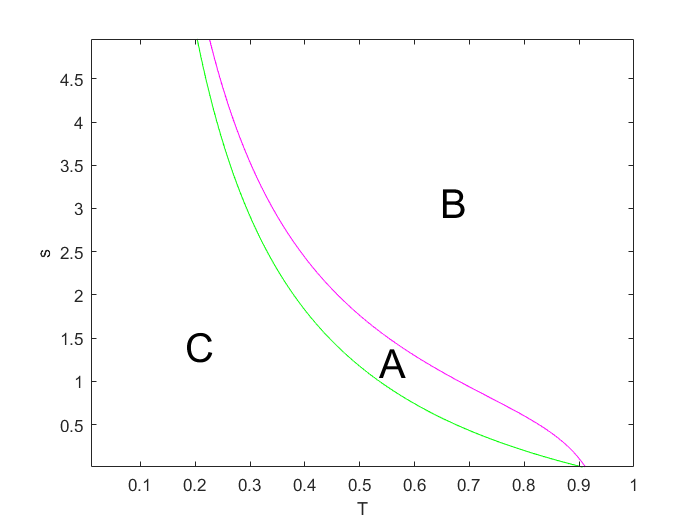
\includegraphics[width=0.33\textwidth]{HLOSimpMutualInvasion1.png} & 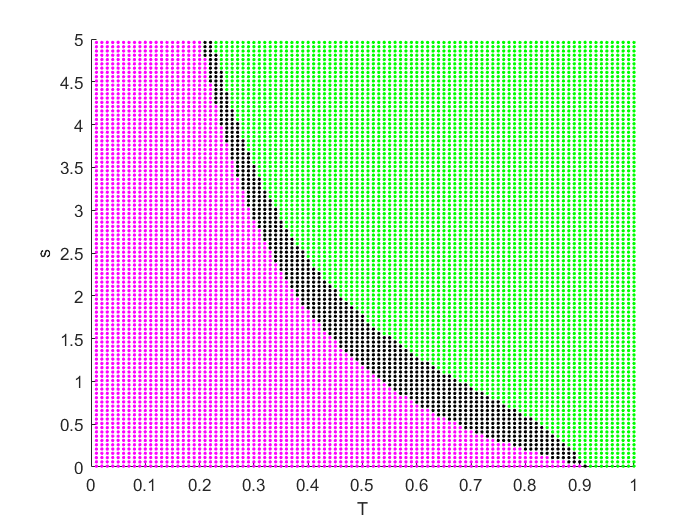
\includegraphics[width=0.33\textwidth]{HLOSimpSSE1.png} & 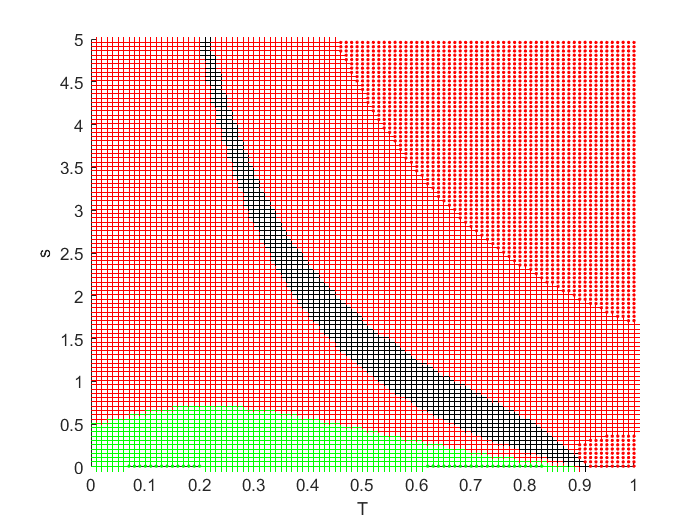
\includegraphics[width=0.33\textwidth]{HLOSimpE1.png}\\
		
		(2) & 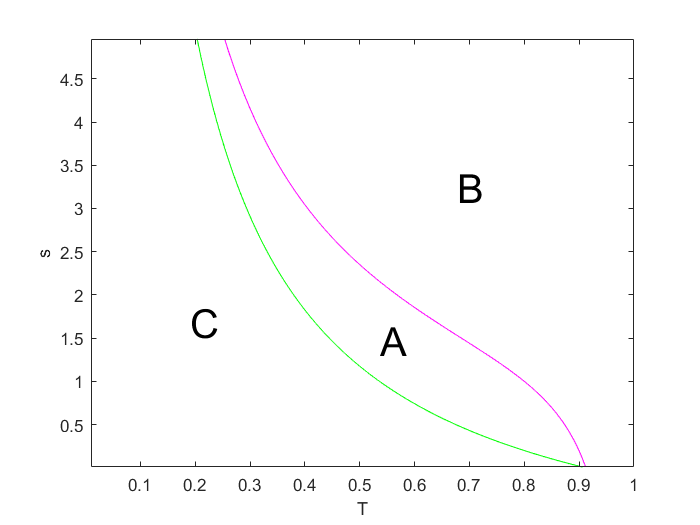
\includegraphics[width=0.33\textwidth]{HLOSimpMutualInvasion2.png} & 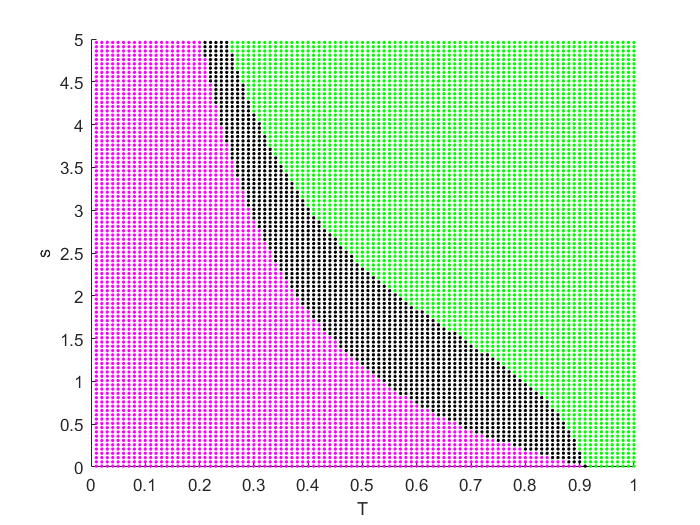
\includegraphics[width=0.33\textwidth]{HLOSimpSSE2.png} & 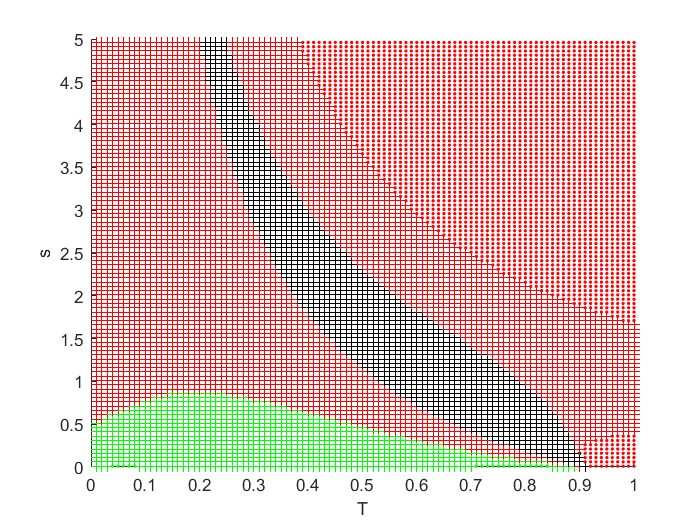
\includegraphics[width=0.33\textwidth]{HLOSimpE2.png}\\
		
		(3) & 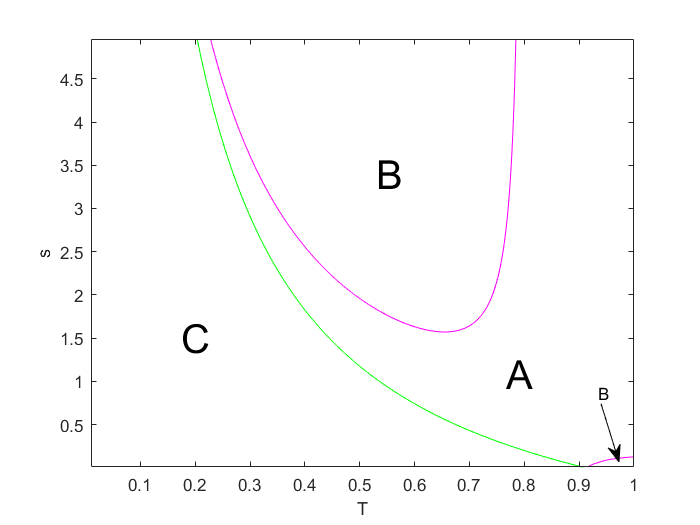
\includegraphics[width=0.33\textwidth]{HLOSimpMutualInvasion3.png} & 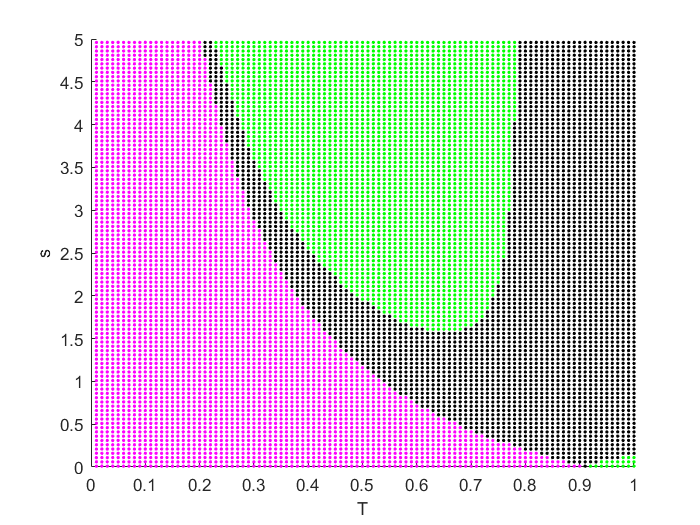
\includegraphics[width=0.33\textwidth]{HLOSimpSSE3.png} & 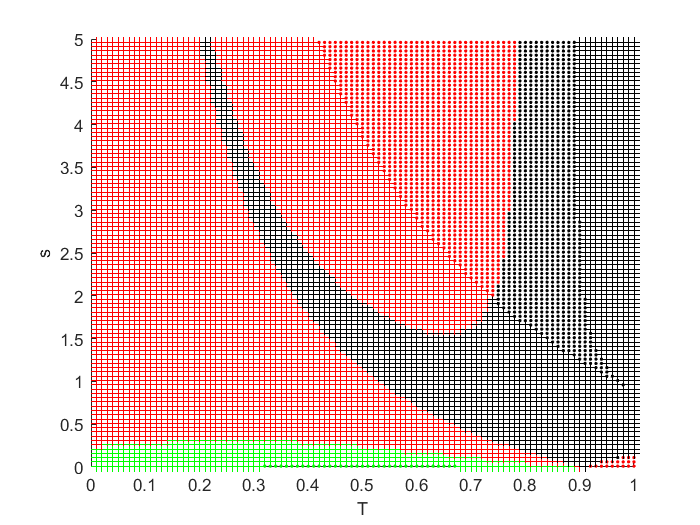
\includegraphics[width=0.33\textwidth]{HLOSimpE3.png}\\
	\end{tabular}
	\caption[Regions for the simplified lynx and owl model]{Coexistence regions for the simplified lynx and owl model (\ref{HLOsimp}). In column (i), only the lynx invades in Regions C, only the owl in Regions B, and we have mutual invasion in Regions A. In column (ii), the equilibrium has three positive components in the black region. Only the owl is non-positive in the magenta region, and only the lynx is non-positive in the green region. In column (iii), three eigenvalues have negative real part in the black region, two in the red region, and all eigenvalues have non-negative real part in the green region. Moreover, imaginary parts are non-zero in the crossed regions and zero in the dotted regions. In row (1), we fix parameters $d=1$, $B=1$, $f=2$, $m=1$, $h=0.5$, $g=1$, $u=1.8$, $b=1$. In row (2), we set $d=0.5$, and in row (3), we set $d=1$ and $B=0.5$.\label{HLOSimpPlots}}%
\end{figure}

Figure \ref{HLOSimpPlots} includes various plots of the regions of interest. We observe that in each row, the regions of mutual invasion (denoted by A in column (i)), positivity of the steady state equations (the black region of column (ii)), and stable steady state (the black region of column (iii)) align exactly. We show this explicitly in Figure \ref{HLOSimpMutualInvasionOnSteadyStateAndEigenvalues}. Row (1) shows that the regions of mutual invasion are identical to the regions of positivity of the steady state. Row (2) shows that the regions of mutual invasion are identical to the regions of stability of the steady state. Therefore, all three regions must be equal, and we observe that mutual invasion implies stable coexistence of all three species.\\
\begin{figure}[h!]
	\centering
	\begin{tabular}{m{0.07cm} m{4.5cm}  m{4.5cm}  m{4.5cm}}
		& \begin{center}
			(i)
		\end{center} & \begin{center}
			(ii)
		\end{center} & \begin{center}
			(iii)
		\end{center}\\
	(1) & 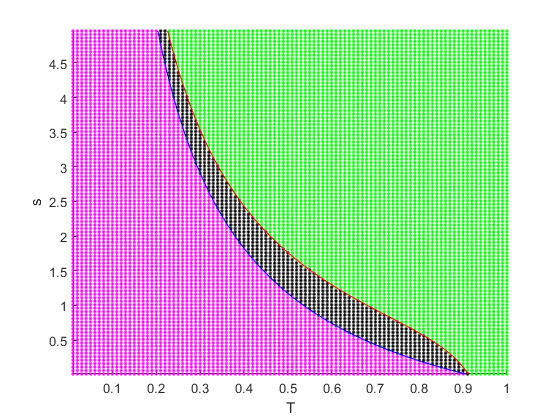
\includegraphics[width=0.33\textwidth]{HLOSimpMutualInvasionOnSteadyState1.png} & 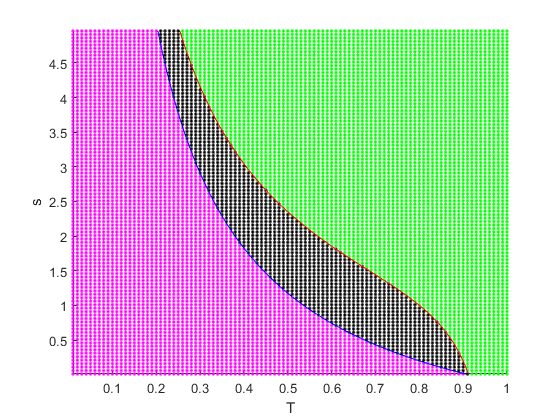
\includegraphics[width=0.33\textwidth]{HLOSimpMutualInvasionOnSteadyState2.png} & 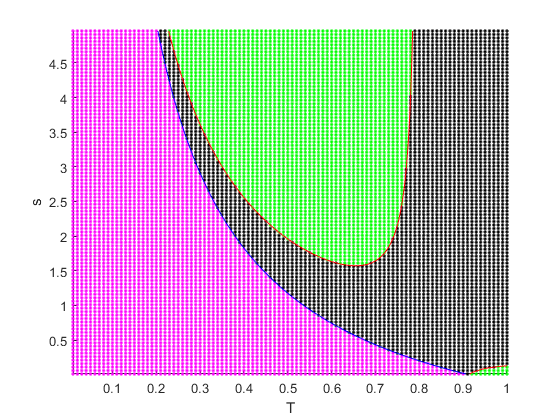
\includegraphics[width=0.33\textwidth]{HLOSimpMutualInvasionOnSteadyState3.png}\\
	(2) & 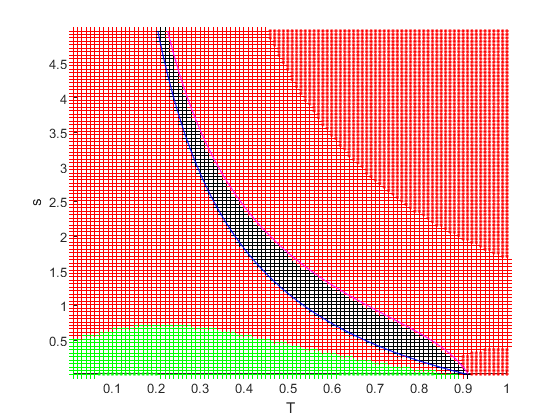
\includegraphics[width=0.33\textwidth]{HLOSimpMutualInvasionOnEigenvalues1.png} & 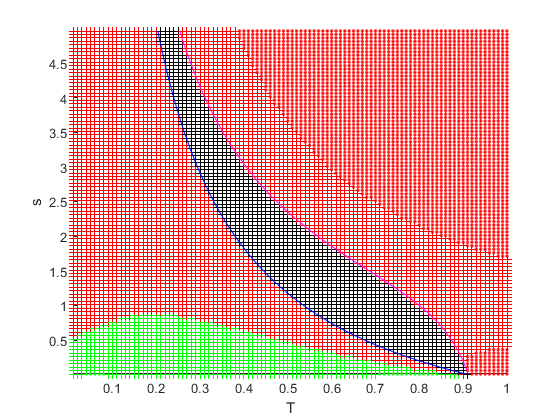
\includegraphics[width=0.33\textwidth]{HLOSimpMutualInvasionOnEigenvalues2.png} & 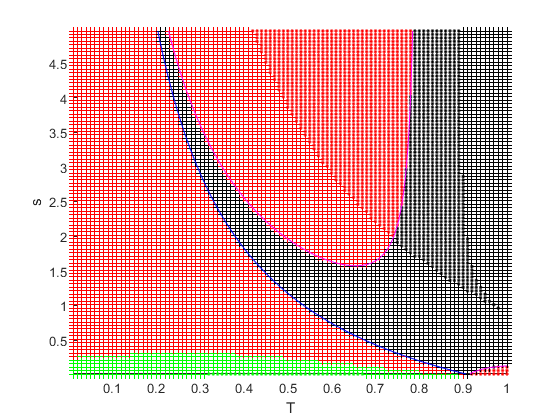
\includegraphics[width=0.33\textwidth]{HLOSimpMutualInvasionOnEigenvalues3.png}
	\end{tabular}
	\caption[Mutual invasion and coexistence in the simplified lynx and owl model]{In row (1), mutual invasion occurs between the blue and red curves, and the steady state (\ref{HLOsimpCoexPt}) is positive in the black region. In row (2), mutual invasion occurs between the blue and magenta curves, and the steady state is stable in the black region. In column (i), we fix parameters $d=1$, $B=1$, $f=2$, $m=1$, $h=0.5$, $g=1$, $u=1.8$, $b=1$. In column (ii), we set $d=0.5$, and in column (iii), we set $d=1$ and $B=0.5$.\label{HLOSimpMutualInvasionOnSteadyStateAndEigenvalues}}%
\end{figure}

In row (2) of Figure \ref{HLOSimpPlots}, we lower the parameter $d$, which represents the hare death rate due to the owl in the winter, and observe how the mutual invasion region changes. We will only talk about the mutual invasion region in this discussion, as we know the stable coexistence region is identical. As we decrease $d$ from $1$ to $0.5$, we notice a change in the magenta curve, which represents the boundary of the lynx invasion region. With a lower death rate due to the owl, the hare density is increased during the winter, which in turn provides a larger amount of resources contributing to the lynx growth. We then expect that the lynx is more likely to persist in the system. This is reflected in the change in the magenta curve. For a fixed $s$, there is a wider range of $T$ for which the lynx can invade because the magenta curve is extended to the right in row (2). This is a direct consequence of the increased hare density. However, this increased hare density occurs only in the winter. As summer length increases, winter dynamics are less influential on annual dynamics, and therefore the lynx will still go extinct beyond a sufficiently large value of $T$.\\

In row (3) of Figure \ref{HLOSimpPlots}, we lower the parameter $B$, which represents the hare death rate due to the owl in the summer, from $1$ to $0.5$. The changes in the mutual invasion region are much more drastic in this case. For lower summer lengths, we do not observe many differences compared to the mutual invasion region in row (1), because we only change a parameter that affects summer dynamics. On the other hand, the region of mutual invasion changes drastically as summer length increases. The intrinsic hare growth rate and lowered death rate in the summer, in conjunction with a longer summer, implies a larger pool of resources for lynx growth that is available for a majority of the year. For values of $T$ roughly between 0.3 and 0.7, the lynx can still go extinct for sufficient large owl growth rates; however, there is a critical value of $T$ beyond which the three species will coexist regardless of owl growth. This is a direct consequence of the greatly increased hare density. We note that, for $s$ close to 0, there is a small region in which we do not obtain coexistence. Once again, this is a region where the lynx cannot invade, so there is only coexistence of the hare and the owl.\\

We summarize the results of this section as follows.
\begin{MainResult}
	Suppose that $0<\frac{m}{f}<1$ and that the following invasion conditions are satisfied:
	\begin{itemize}
		\item $T\left(h\left(\frac{m}{f}\right)^2+s\right)+(1-T)\left(\frac{gm}{f}-u\right)>0$,
		\item $f\tilde{x}-m>0,$
	\end{itemize}
	 where $\tilde{x}$ is the $x$-component of the unique positive stable steady state found in Theorem \ref{TheoHOSimpCoex}. Then there exists a unique stable positive steady state for (\ref{HLOsimp}), given by equation (\ref{HLOsimpCoexPt}).
	\label{TheoHLOSimpMutInvCoex}
\end{MainResult}

For every choice of parameters we make, we observe that mutual invasion implies coexistence. When studying other simplifications of original model (\ref{HLO}), as well as the original model itself, we will use this approach to look for regions of coexistence. Although the implication of coexistence due to mutual invasion is difficult to prove analytically, the approach presented in this chapter is applicable to all models in which we can find mutual invasion conditions, as well as calculate an explicit non-trivial steady state. We will see that this is the case in the following section, where we simplify only the owl terms in (\ref{HLO}).\\

We end this section on a note about the MATLAB scripts used to generate plots in Figure \ref{HLOSimpPlots} and all similar plots in this thesis. We use two general structures of MATLAB scripts, one that corresponds to the regions of mutual invasion, and one that corresponds to the regions of positivity and stability of the steady state.\\

In the first case, we create a 98-by-99 grid over a region of the positive quadrant of the $(T,s)$-plane. The idea is to establish a 100-by-100 array over the region, but we ignore the values $T=0$, $T=1$ and $s=0$ because each case causes singularities in either the model equations or the Jacobian of the system. Moreover, the vertical size of the array may change according to the values of $s$ we consider; however, we remain on the order of 100. Once our array is established, we run a double loop over the grid and for each point $(T,s)$ on the array, we calculate the lynx and owl invasion conditions, respectively (\ref{HLOsimpLynxInvCond}) and (\ref{HLOsimpOwlInvCond}), and we create two new arrays that correspond to the values of the owl and lynx conditions. For conditions that involve a steady-state value, we either have an analytic expression for the value or we do not. In the latter case, we either use the \textit{roots} function if the value is given by a polynomial of degree $\ge 2$, or we integrate the system using the \textit{ode45} function until we are at a steady state. For sampled values of $T$ and $s$, we find approximate times until we are at the steady state; i.e., when values do not change up to fourth decimal order. By default, the solver would not give higher-order precision on integrated solutions. In some cases, however, we reduced the relative tolerance to $10^{-8}$ and the absolute tolerance to $10^{-6}$.\\

If invasion conditions are defined as the integral along a periodic solution, we solve the ODE with \textit{ode45} until we are on a periodic orbit. We do so the same way as above, by choosing a run time that is an order of magnitude above the sampled run times. After the initial run time, we integrate the system again for a different run time, and we create a \textit{while} loop that counts the peaks in one component of the solution using the \textit{findpeaks} function; if the number of peaks is less than 2, we extend the second run time and try again. Once we have at least two peaks, we extract the data of the solution between two peaks, which gives us one orbit around the periodic solution. We note that it is sufficient to only check the peaks without comparing the entire solution between the peaks. This is because uniqueness of solutions: if two solutions agree at a common peak, they must be identical everywhere. We can then use this data in the invasion conditions. We note that there are always some tolerance errors, which result in the peaks occurring at exactly the same height. However, we found that the solution repeats after each peak, and we do not have periodic solutions that exhibit multiple peaks in a single period. Therefore, we know that, between any two peaks, we will obtain one full period of the solution, and error resulting from the difference in peak heights is negligible with respect to the invasion conditions. After obtaining one period of the solution, we calculate the integrals in the invasion conditions using the \textit{trapz} function. Once the invasion-condition arrays are complete, we use the \textit{contour} function to obtain the green and magenta curves in the left column of Figure \ref{HLOSimpPlots}.\\

In the second case, we create an identical array of a region of the positive $(T,s)$-plane. In every model we encounter, we have an explicit expression for the coexistence steady state. Therefore, at each point $(T,s)$ in the array, once again via a double loop, we compute these expressions. We then check if any components of the expression are strictly positive, and the amount of such components determine the corresponding colour of the point. We then plot the point in column (ii) of Figure \ref{HLOSimpPlots}. Finally, we can write analytic expression for the Jacobian matrix and use the \textit{eig} function to find eigenvalues. We check which eigenvalues have strictly negative real part and non-zero imaginary part, which determines the colour of the point. We then plot the point in column (iii) of Figure \ref{HLOSimpPlots}.\\

For comparison plots such as Figure \ref{HLOSimpMutualInvasionOnSteadyStateAndEigenvalues}, we simply combine both of the above scripts into one and display results on the same plot. All plots in this thesis are created identically. If there is an analytic inequality to satisfy, we use the \textit{contour} function; otherwise, we use plots with coloured points to define specific regions in $(T,s)$-space.\\

\section{Simplified Owl Model}
\label{SectionSimpOwl}

The simplifications made in the previous section allowed us to arrive at some interesting results regarding the relationship between seasonality and coexistence in the three-species model. In this section, we will only simplify the owl terms in the focal model and proceed with invasion analysis as we did in the previous section. After simplification and non-dimensionalization, the simplified owl model reads
\begin{equation}
	\begin{split}
		&\dot{x}=T\Big(x(1-x)-\frac{xy}{b+kx}-a x^2z\Big)+(1-T)\Big(-\frac{xy}{b+kx}-d xz\Big),\\
		&\dot{y}=\frac{fxy}{b+kx}-my,\\
		&\dot{z}=T\Big(hx^2z+sz(1-z)\Big)+(1-T)\Big(gxz-uz\Big).
	\end{split}
	\label{HLOOwlSimp}
\end{equation}

The hare--owl subsystem is identical to the previous case (\ref{HOsimp}), but with parameter $a$ replacing parameter $B$. We use Theorem \ref{TheoHOSimpCoex} to determine when we have coexistence in this subsystem. The conditions in terms of the current parameters are
\begin{equation}
	\begin{split}
		\text{(i)}&\ \frac{T}{(1-T)d}>\frac{1}{Ts}\Big(Ts-(1-T)u\Big),\\
		\text{(ii)}&\ \frac{1}{Ts}\Big(T(h+s)+(1-T)(g-u)\Big)>0.
	\end{split}
	\label{HLOOwlSimpHOCoexCond}
\end{equation}

Under these conditions, there is a stable steady state $(x^*,0,z^*)$ of the hare--owl subsystem. At this state, the lynx equation of the linearised system decouples as
$$\dot{y}=\left(\frac{fx^*}{b+kx^*}-m\right)y.$$
Therefore, the lynx invasion condition is
\begin{equation}
	\frac{fx^*}{b+kx^*}-m>0.
	\label{HLOOwlSimpLynxInvCond}
\end{equation}

We now determine owl-invasion conditions. Setting $z=0$ in (\ref{HLOOwlSimp}), we obtain

\begin{equation}
\begin{split}
&\dot{x}=Tx(1-x)-\frac{xy}{b+kx},\\
&\dot{y}=\frac{fxy}{b+kx}-my,\\
&\dot{z}=0.
\end{split}
\label{HLOOwlSimpz=0}
\end{equation}

The hare--lynx subsystem of (\ref{HLOOwlSimpz=0}) is a classical Rosenzweig-MacArthur model \cite{RosMac}, and the dynamics of this model are well understood. If
$$0<\frac{mb}{f-mk}<1,$$
there exists a unique hare--lynx coexistence state, given by
\begin{equation}
(x^*,y^*,0)=\left(\frac{mb}{f-mk}, T(1-x^*)(b+kx^*),0\right).
\label{HLOOwlSimpRMSS}
\end{equation}
To determine stability of this steady state, we can follow the method from \cite{Kot}. In particular, we can rewrite (\ref{HLOOwlSimp}) as
\begin{equation}
	\begin{split}
		\dot{x}=& h(x)\left[g(x)-y\right],\\
		\dot{y}=& f\left[h(x)-\frac{m}{f}\right]y,
	\end{split}
	\label{HLOOwlSimpRMKot}
\end{equation}
where
$$h(x)=\frac{x}{b+kx},\hspace{0.5in}\text{ and }\hspace{0.5in} g(x)=T(1-x)(b+kx).$$
We note that $y^*=g(x^*)$. The Jacobian of (\ref{HLOOwlSimpRMKot}) evaluated at the steady state (\ref{HLOOwlSimpRMSS}) is given by
\begin{equation}
	\begin{pmatrix}
	\frac{m}{f}g'(x^*) & -\frac{m}{f}\\ \\
	fh'(x^*)g(x^*) & 0
	\end{pmatrix}.
	\label{RosMacJac}
\end{equation}
Since $g(x^*)=y^*$ and $h(x)$ is an increasing function of $x$, the determinant of (\ref{RosMacJac}) is positive. Hence, the steady state is stable if the trace is negative and unstable when it is positive. We study the bifurcation that occurs when the trace is zero in more detail. The characteristic equation
$$\lambda^2-\frac{m}{f}g'(x^*)\lambda+mh'(x^*)g(x^*)=0,$$
has complex conjugate roots when the trace is near zero; i.e., when $|\frac{m}{f} g'(x^*)|$ is small. These roots are given explicitly by
\begin{equation}
	\lambda=\frac{m}{2f}g'(x^*)\pm i\sqrt{mh'(x^*)g(x^*)-\left(\frac{m}{2f}g'(x^*)\right)^2}.
	\label{HLOOwlSimpRMEvals}
\end{equation}
We apply Theorem \ref{TheoHopfBIf} and define a new parameter $\alpha=g'(x^*)=f(k-b)-mk(k+b)$ and study the bifurcation that occurs when $\alpha$ passes through 0.
With functions $h(x)$ and $g(x)$ defined as above, we can rewrite (\ref{HLOOwlSimpRMEvals}) as
$$\lambda=\mu(\alpha)\pm i\nu(\alpha)=\frac{Tm}{2f(f-mk)}\alpha\pm i\sqrt{\frac{Tm}{fk}(\alpha+fb)-\left(\frac{Tm}{2f(f-mk)}\alpha\right)^2}.$$
With the eigenvalues written in this form, we have
\begin{flalign*}
	\mu(0)&=0,\\
	\mu'(0)&=\frac{Tm}{2f(f-mk)}\ne 0,\\
	\nu(0)&=\sqrt{\frac{Tmb}{k}}>0.
\end{flalign*}
The second and third expressions hold because all parameters are strictly positive. Moreover, for the steady state (\ref{HLOOwlSimpRMSS}) to be defined, we need $f-mk\ne0$, so $\mu'(0)$ is well-defined. These three conditions are precisely the genericity conditions for a Hopf bifurcation at $\alpha=f(k-b)-mk(k+b)=0$ \cite{Kuznetsov}. We can further classify the bifurcation by looking at the signs of the term $\mu'(0)$ as well as the \textit{first Lyapunov coefficient}. This is an important quantity, which appears in the application of normal-form theory to the Taylor expansion of (\ref{HLOOwlSimpz=0}) around the steady state (\ref{HLOOwlSimpRMSS}). The sign of the first Lyapunov coefficient specifies the stability types of the steady state and limit cycles resulting form a Hopf bifurcation. More details can be found in \cite{Kuznetsov}. \\

In the biological framework of this model, the coexistence steady state (\ref{HLOOwlSimpRMSS}) must satisfy $x^*>0$ and $y^*>0$. Therefore, we require $f-mk>0$ so the term $\mu'(0)$ is positive. This means that, for
\begin{equation}
	f(k-b)-mk(k+b)<0,
	\label{HLOOwlSimpRMCond}
\end{equation}
there are no limit cycles, but, as this quantity passes through zero and becomes positive, we observe a change in stability of the steady state (\ref{HLOOwlSimpRMSS}) from which limit cycles emerge of the opposite stability type. To determine stability of the limit cycles, we can compute the sign of the first Lyapunov coefficient, or we can integrate the system for cases where condition (\ref{HLOOwlSimpRMCond}) is satisfied and cases where it is not and observe the stability types. For example, from Figures 8.11 and 8.12 in \cite{Kot}, we see that the steady state is stable under condition (\ref{HLOOwlSimpRMCond}) and becomes unstable as this condition is reversed, leading to stable limit cycles. We can now proceed with owl invasion at the steady state (\ref{HLOOwlSimpRMSS}) while considering two cases separately: invasion at a steady state and invasion at a periodic orbit.\\

\subsubsection*{Case 1: Owl invasion at a steady state}

We know that the coexistence steady state (\ref{HLOOwlSimpRMSS}) is stable in system (\ref{HLOOwlSimpz=0}) under condition (\ref{HLOOwlSimpRMCond}). For this case, we suppose this condition is satisfied, as well as the condition
$$0<\frac{mb}{f-mk}<1,$$
which ensures that the quantities $x^*$ and $y^*$ are positive. Under these conditions, the owl equation in the linearised system at $(x^*,y^*,0)$ decouples yet again. Therefore, the state $(x^*,y^*,0)$ is unstable in the $z$ direction when
\begin{equation}
	T\left(h\left(\frac{mb}{f-mk}\right)^2+s\right)+(1-T)\left(g\frac{mb}{f-mk}-u\right)>0.
	\label{HLOOwlSimpOwlSSInvCond}
\end{equation}
This is our owl-invasion condition at steady state.\\

As in the previous chapter, we proceed with a numerical evaluation and illustration of coexistence in (\ref{HLOOwlSimp}). This is possible because we can explicitly calculate the unique positive steady state
\begin{equation}
	\begin{split}
		x^*&=\frac{mb}{f-mk},\\
		y^*&=\Big(b+kx^*\Big)\Big(T(1-x^*-ax^*z^*)-(1-T)dz^*\Big)\\
		z^*&=\frac{1}{Ts}\Big(T(h(x^*)^2+s)+(1-T)(gx^*-u)\Big).
	\end{split}
	\label{HLOOwlSimpSteadyState}
\end{equation}
We vary parameters $T$ and $s$ while the remaining parameters are fixed, and we observe whether or not regions of mutual invasion, positivity of steady state (\ref{HLOOwlSimpSteadyState}) and stability of the steady state overlap. These regions are included in Figure \ref{HLOOwlSimpSSPlots}. All parameters are fixed and given in the figure, except for the parameter $u$. We vary this parameter across each row of the figure; we set $b=1$ in the row (1), $b=0.9$ in row (2) and $b=0.9$ in row (3).\\
\begin{figure}[h!]
	\centering
	\begin{tabular}{m{0.07cm} m{4.5cm}  m{4.5cm}  m{4.5cm}}
		& \begin{center}
			(i)
		\end{center} & \begin{center}
		(ii)
		\end{center} & \begin{center}
		(iii)
		\end{center}\\
		(1) & 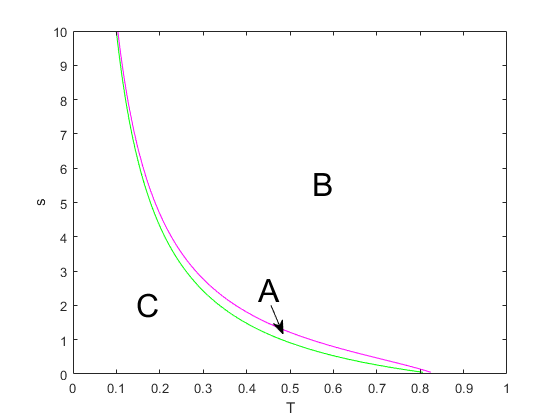
\includegraphics[width=0.33\textwidth]{HLOOwlSimpSSMutualInvasion1.png} & 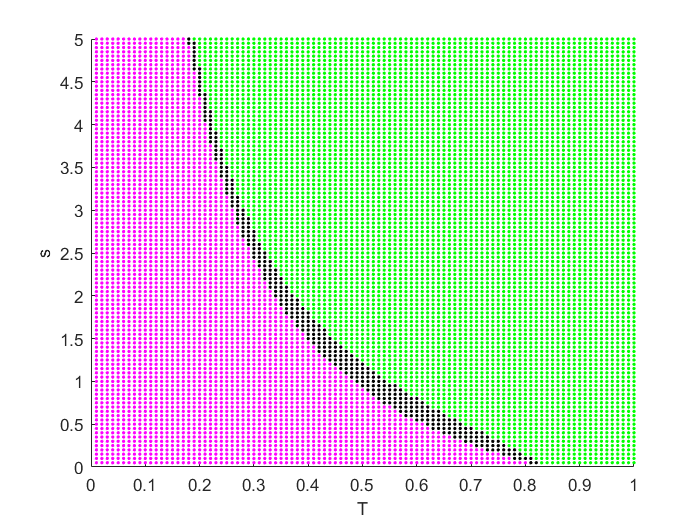
\includegraphics[width=0.33\textwidth]{HLOOwlSimpSSSteadyState1.png} & 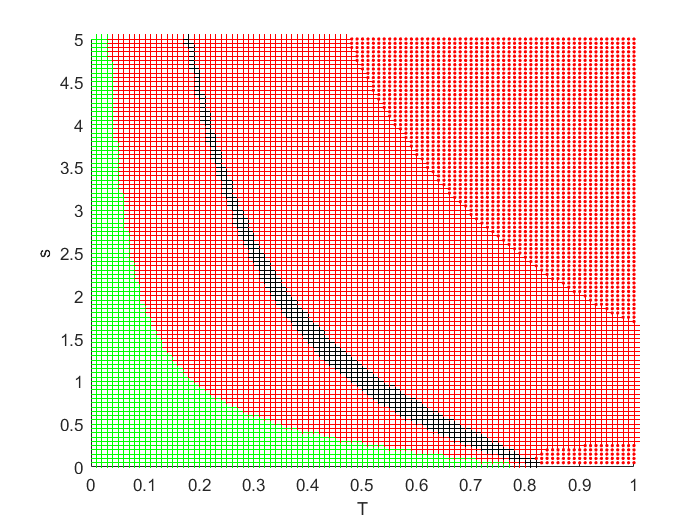
\includegraphics[width=0.33\textwidth]{HLOOwlSimpSSEigenvalues1.png}\\
		
		(2) & 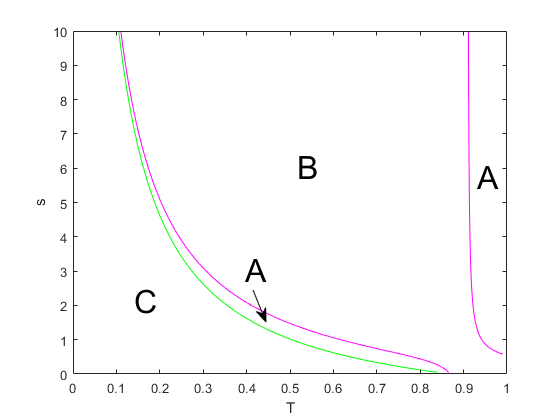
\includegraphics[width=0.33\textwidth]{HLOOwlSimpSSMutualInvasion2.png} & 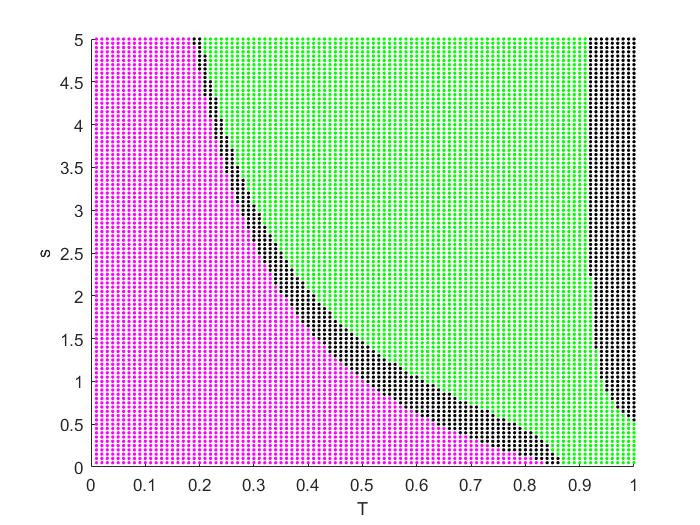
\includegraphics[width=0.33\textwidth]{HLOOwlSimpSSSteadyState2.png} & 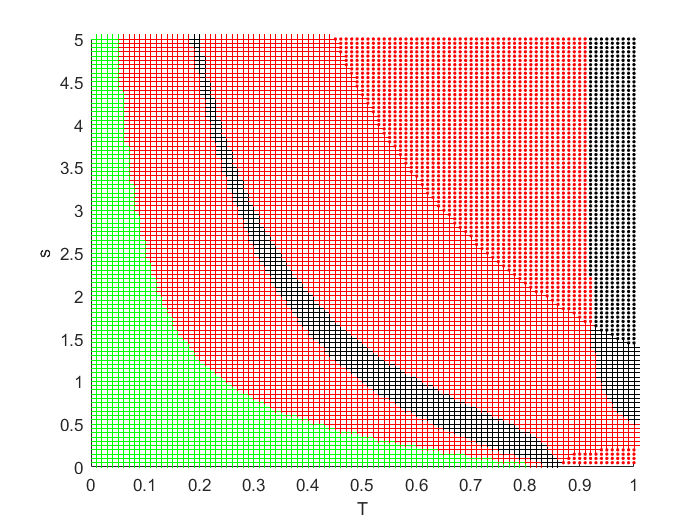
\includegraphics[width=0.33\textwidth]{HLOOwlSimpSSEigenvalues2.png}\\
		
		(3) & 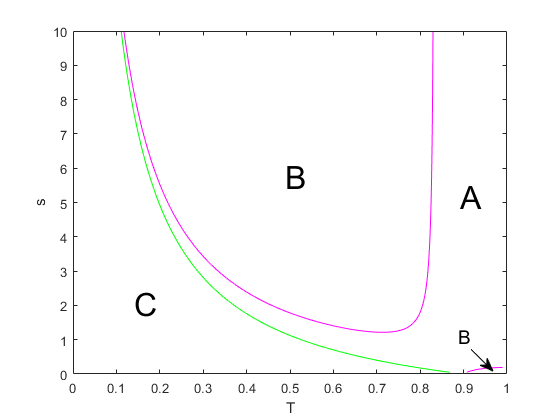
\includegraphics[width=0.33\textwidth]{HLOOwlSimpSSMutualInvasion3.png} & 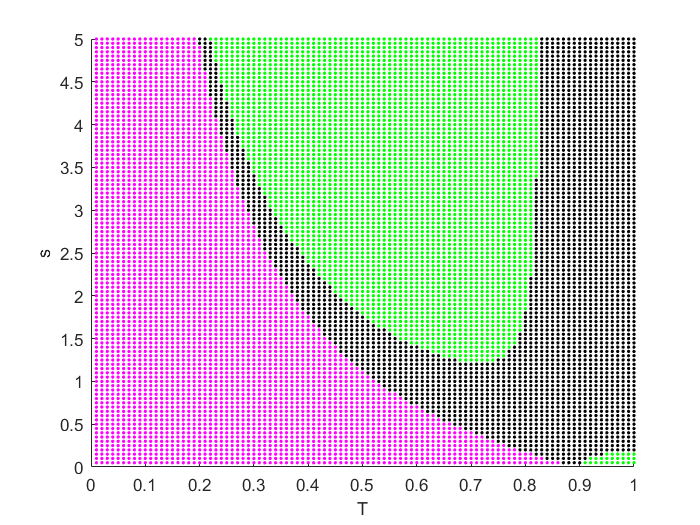
\includegraphics[width=0.33\textwidth]{HLOOwlSimpSSSteadyState3.png} & 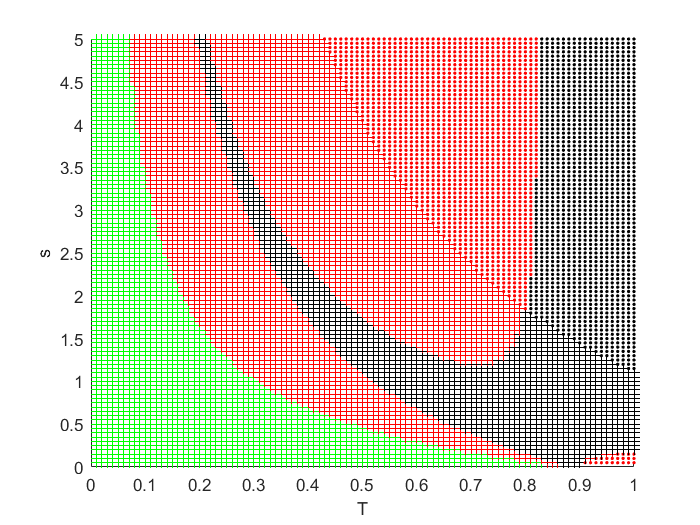
\includegraphics[width=0.33\textwidth]{HLOOwlSimpSSEigenvalues3.png}\\
	\end{tabular}
	\caption[Regions for the simplified owl model (steady state)]{Coexistence regions for the simplified owl model (\ref{HLOOwlSimp}), given at steady state in the hare--lynx submodel (\ref{HLOOwlSimpz=0}). In column (i), only the lynx invades in Regions C, only the owl in Regions B and we have mutual invasion in Regions A. In column (ii), the equilibrium has three positive components in the black region. Only the owl term is non-positive in the magenta region, and only the lynx term is non-positive in the green region. In column (iii), three eigenvalues have negative real part in the black region, two in the red region, one in the cyan region, and all eigenvalues have non-negative real part in the green region. Moreover, imaginary parts are nonzero in the crossed regions, and zero in the dotted regions. In row (1), we fix parameters $k=0.5$, $d=1$, $a=0.5$, $b=1$, $f=2$, $m=1$, $h=0.5$, $g=1$, $u=1.8$. In row (2), we set $b=0.9$, and in row (3), we set $b=0.8$.\label{HLOOwlSimpSSPlots}}%
\end{figure}

We observe that the regions of mutual invasion, denoted by A in column (i), are identical to the regions in which the steady state is positive. We highlight this in the row (1) of Figure \ref{HLOOwlSimpSSMutualInvasionOnSteadyStatesAndEigenvalues}. The region of mutual invasion lies between the blue and red curves, whereas the black region represents positivity of the steady state. We can also compare mutual invasion and stability of the steady state in an identical way. This is shown in row (2) of the same figure. We then see that the regions of mutual invasion, between the blue and magenta curves, are identical to the regions where the steady state (\ref{HLOOwlSimpSteadyState}) is stable. Therefore, mutual invasion implies stable coexistence at a steady in (\ref{HLOOwlSimp}) when the hare--lynx system has a stable steady state.

\begin{figure}[h!]
	\centering
	\begin{tabular}{m{0.07cm} m{4.5cm}  m{4.5cm}  m{4.5cm}}
		& \begin{center}
			(i)
		\end{center} & \begin{center}
			(ii)
		\end{center} & \begin{center}
			(iii)
		\end{center}\\
		(1) & 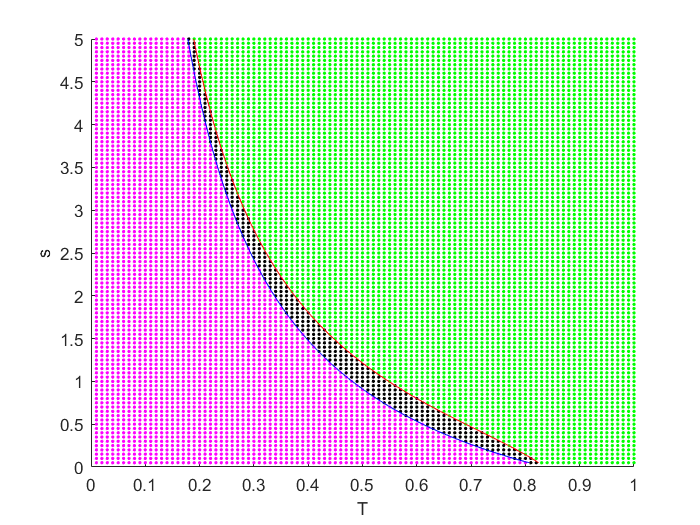
\includegraphics[width=0.33\textwidth]{HLOOwlSimpSSMutualInvasionOnSteadyState1.png} & 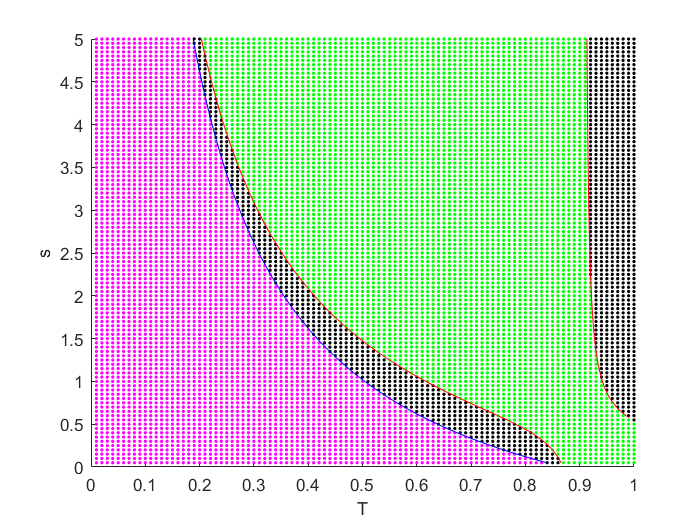
\includegraphics[width=0.33\textwidth]{HLOOwlSimpSSMutualInvasionOnSteadyState2.png} & 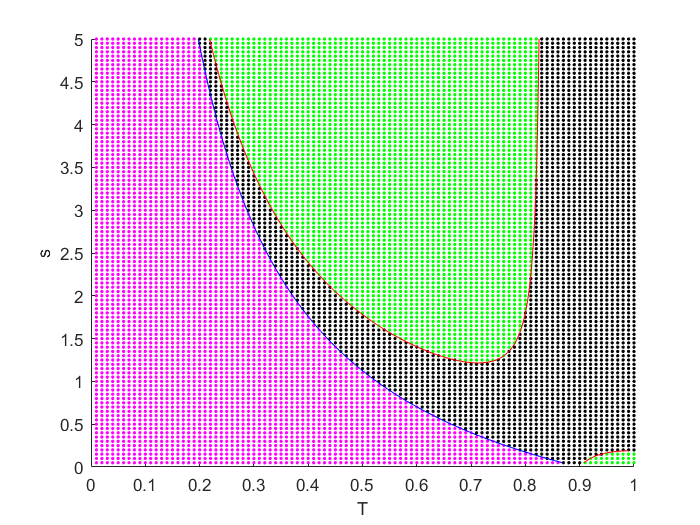
\includegraphics[width=0.33\textwidth]{HLOOwlSimpSSMutualInvasionOnSteadyState3.png}\\
		
		(2) & 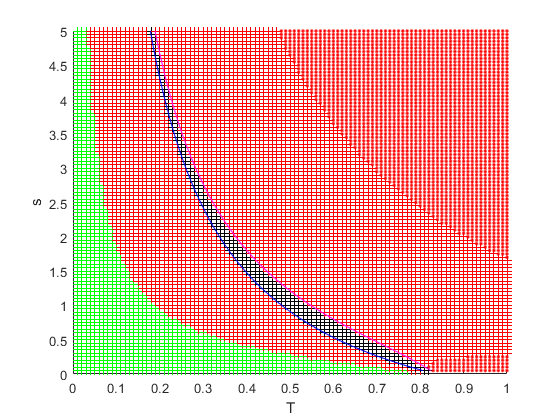
\includegraphics[width=0.33\textwidth]{HLOOwlSimpSSMutualInvasionOnEigenvalues1.png} & 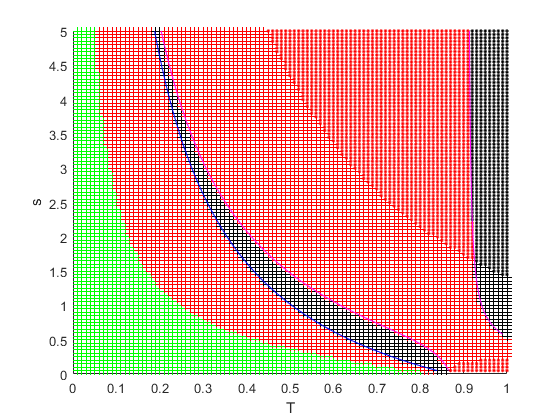
\includegraphics[width=0.33\textwidth]{HLOOwlSimpSSMutualInvasionOnEigenvalues2.png} & 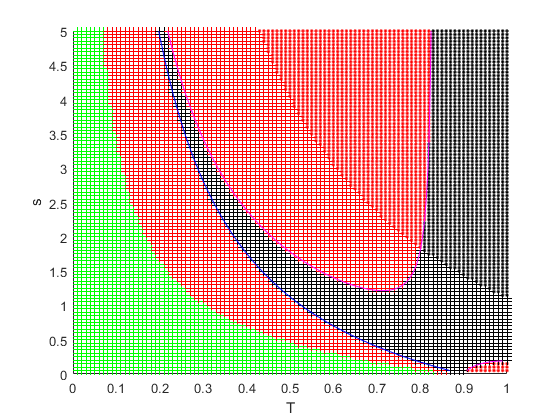
\includegraphics[width=0.33\textwidth]{HLOOwlSimpSSMutualInvasionOnEigenvalues3.png}\\
	\end{tabular}
	\caption[Mutual invasion and coexistence in the simplified owl model (steady state)]{In row (1), mutual invasion occurs between the blue and red curves, and the steady state (\ref{HLOOwlSimp}) is positive in the black region. In row (2), mutual invasion occurs between the blue and magenta curves, and the steady state is stable in the black region. In column (i), we fix parameters $k=0.5$, $d=1$, $a=0.5$, $b=1$, $f=2$, $m=1$, $h=0.5$, $g=1$, $u=1.8$. In column (ii), we set $b=0.9$, and in column (iii), we set $b=0.8$.\label{HLOOwlSimpSSMutualInvasionOnSteadyStatesAndEigenvalues}}%
\end{figure}

\subsubsection*{Case 2: Owl invasion at a periodic orbit}

We now consider the case when condition (\ref{HLOOwlSimpRMCond}) is reversed in system (\ref{HLOOwlSimpz=0}). We know that, as this quantity passes from negative to positive, the steady state (\ref{HLOOwlSimpRMSS}) loses stability via a Hopf bifurcation, and we obtain a stable periodic orbit. We will denote this orbit by $(x^*(t),y^*(t),0)$ and its period by $\tau$. In this case, the $z$ equation in the linearisation of (\ref{HLOOwlSimp}) at the periodic orbit $(x^*(t),y^*(t),0)$ decouples as
$$\dot{z}=\left[T\left(hx^*(t)^2+s\right)+(1-T)(gx^*(t)-u)\right]z=\colon A(t)z.$$
Since $A(t)$ is periodic of period $\tau$ in $t$, we are in the framework of Floquet theory. By Theorem \ref{TheoOneDimFLoquet}, we know that the orbit $(x^*(t),y^*(t),0)$ is unstable in the $z$ direction precisely when
\begin{equation}
	\frac{1}{\tau}\int_0^\tau A(t)\ dt=\frac{1}{\tau}\int_0^\tau \left[T\left(hx^*(t)^2+s\right)+(1-T)(gx^*(t)-u)\right]\ dt>0.
	\label{HLOOwlSimpOwlPOInvCond}
\end{equation}
This is the owl-invasion condition for the periodic orbit. We proceed with the same analysis as in the previous case, with the exception of a new owl-invasion condition. For this case, it will be necessary to numerically integrate the system (\ref{HLOOwlSimpz=0}) to obtain the periodic orbit before we can determine regions of mutual invasion, positivity and stability of the steady state (\ref{HLOOwlSimpSteadyState}). Otherwise, the procedure is identical. These regions are included in Figure \ref{HLOOwlSimpPOPlots}. All parameters are fixed and given in the figure, except for the parameter $u$. We vary this parameter across each row of the figure; we set $u=0.8$ in row (1), $u=0.5$ in the second and $u=0.2$ in the third.\\

\begin{figure}[h!]
	\centering
	\begin{tabular}{m{0.07cm} m{4.5cm}  m{4.5cm}  m{4.5cm}}
		& \begin{center}
			(i)
		\end{center} & \begin{center}
			(ii)
		\end{center} & \begin{center}
			(iii)
		\end{center}\\
		(1) & 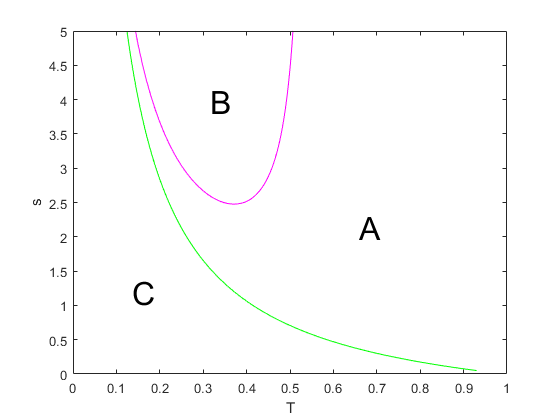
\includegraphics[width=0.33\textwidth]{HLOOwlSimpPOMutualInvasion1.png} & 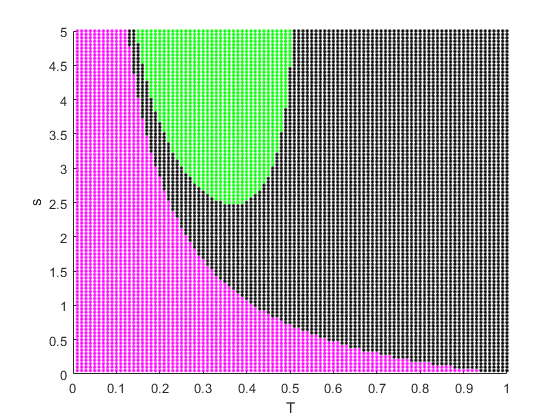
\includegraphics[width=0.33\textwidth]{HLOOwlSimpPOSteadyState1.png} & 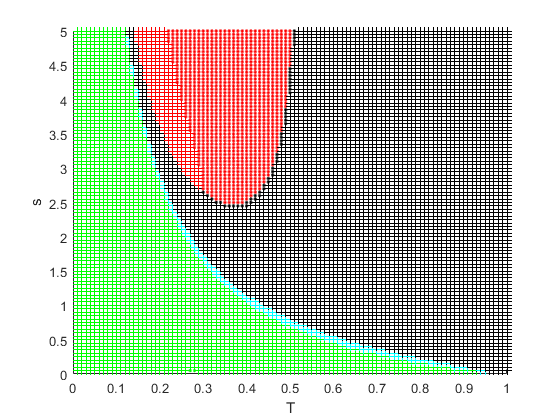
\includegraphics[width=0.33\textwidth]{HLOOwlSimpPOEigenvalues1.png}\\
		
		(2) & 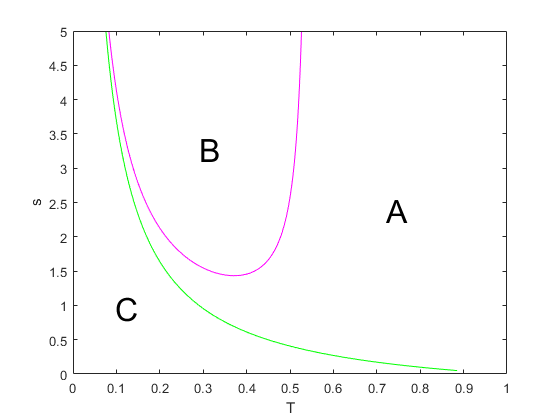
\includegraphics[width=0.33\textwidth]{HLOOwlSimpPOMutualInvasion2.png} & 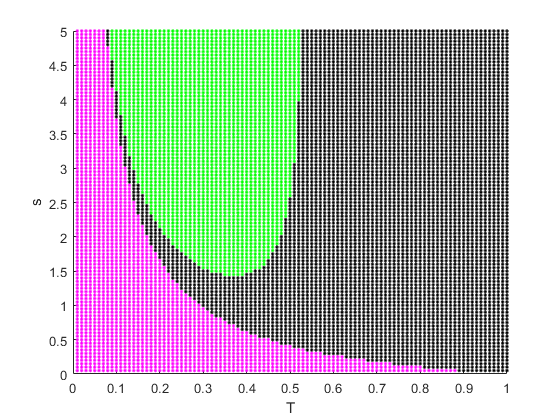
\includegraphics[width=0.33\textwidth]{HLOOwlSimpPOSteadyState2.png} & 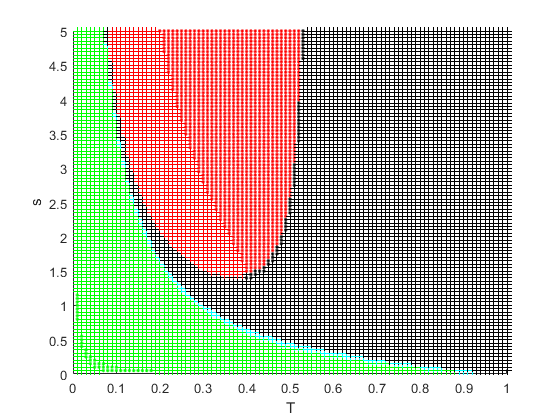
\includegraphics[width=0.33\textwidth]{HLOOwlSimpPOEigenvalues2.png}\\
		
		(3) & 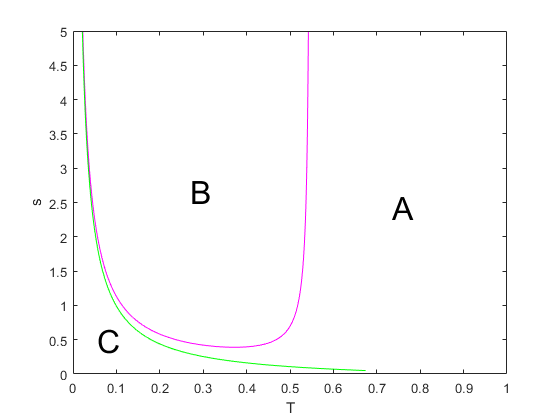
\includegraphics[width=0.33\textwidth]{HLOOwlSimpPOMutualInvasion3.png} & 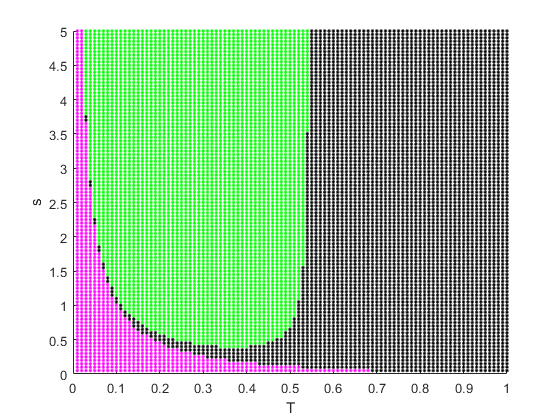
\includegraphics[width=0.33\textwidth]{HLOOwlSimpPOSteadyState3.png} & 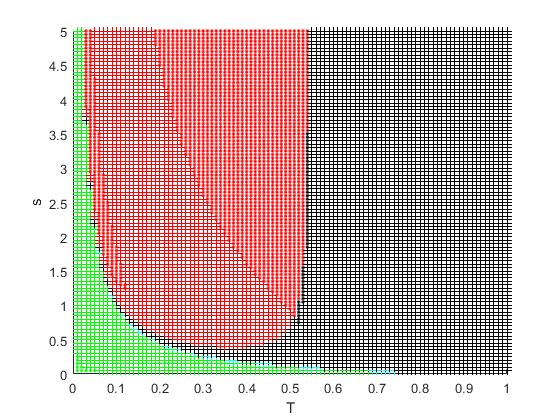
\includegraphics[width=0.33\textwidth]{HLOOwlSimpPOEigenvalues3.png}\\
	\end{tabular}
	\caption[Regions for the simplified owl model (periodic orbit)]{Coexistence regions for the simplified owl model (\ref{HLOOwlSimp}), given a periodic orbit in the hare--lynx system (\ref{HLOOwlSimpz=0}). In column (i), only the lynx invades in Regions C, only the owl in Regions B and we have mutual invasion in Regions A. In column (ii), the equilibrium has three positive components in the black region. Only the owl term is non-positive in the magenta region, and only the lynx term is non-positive in the green region. In column (iii), three eigenvalues have negative real part in the black region, two in the red region, one in the cyan region, and all eigenvalues have non-negative real part in the green region. Moreover, imaginary parts are non-zero is the crossed regions and zero in the dotted regions. In row (1), we fix parameters $k=0.9$, $d=1$, $a=1$, $b=0.5$, $f=2$, $m=0.3$, $h=0.3$, $g=1$, $u=0.8$. In row (2), we set $u=0.5$, and in row (3), we set $u=0.2$.\label{HLOOwlSimpPOPlots}}%
\end{figure}

In Figure \ref{HLOOwlSimpPOMutualInvasionOnSteadyStatesAndEigenvalues}, we observe the relationship between mutual invasion and positivity of the steady state in this case. Row (1) shows that regions of mutual invasion between the blue and red curves are identical to regions where the steady state (\ref{HLOOwlSimpSteadyState}) is positive, in black. In row (2), however, the regions of mutual invasion, between the blue and magenta curves, do not align with the black regions, which represent where the steady state is stable. The difference is there is a cyan region contained within the region of mutual invasion. The cyan region corresponds to two eigenvalues with non-negative real part at the steady state (\ref{HLOOwlSimpSteadyState}). In fact, there is a complex conjugate pair of eigenvalues indicated by a crossed cyan region rather than dotted. By integrating the system (\ref{HLOOwlSimp}) in this region, we find periodic solutions (middle plot of Figure \ref{HLOOwlSimpPOCyanSolutions}). As we enter the black region, however (right plot of Figure \ref{HLOOwlSimpPOCyanSolutions}), the oscillations die out, and we are left with a stable steady state. This is indicative of a supercritical Hopf bifurcation along the boundary of the cyan and black regions. In the green region, solutions are periodic in the hare--lynx system as expected in this case. This is shown in the left plot of the same figure. Therefore, owl invasion results in a periodic solution for sufficiently small $s$ and $T$ and stable steady state for larger values. We note that the parameter $s$ measures the owl growth rate due to alternative resources, and, as $T$ increases, more alternative resources are available. The observed effect of the combination of these phenomena is that the presence of the owl dampens the oscillations in the hare--owl system to the point where they disappear completely, resulting in the stable steady state.\\

\begin{figure}[h!]
	\centering
	\begin{tabular}{m{0.07cm} m{4.5cm}  m{4.5cm}  m{4.5cm}}
		& \begin{center}
			(i)
		\end{center} & \begin{center}
			(ii)
		\end{center} & \begin{center}
			(iii)
		\end{center}\\
		(1) & 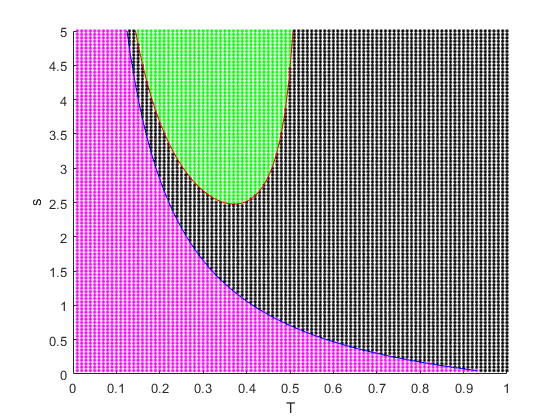
\includegraphics[width=0.33\textwidth]{HLOOwlSimpPOMutualInvasionOnSteadyState1.png} & 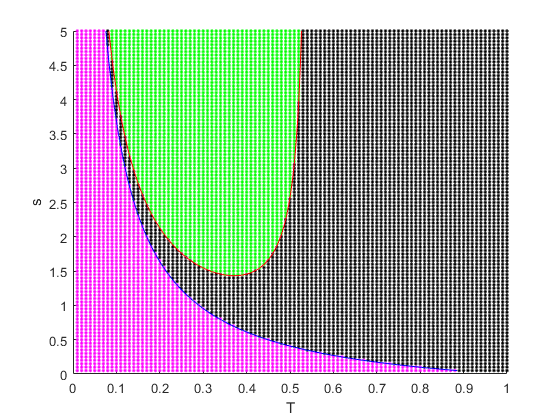
\includegraphics[width=0.33\textwidth]{HLOOwlSimpPOMutualInvasionOnSteadyState2.png} & \includegraphics[width=0.33\textwidth]{HLOOwlSimpPOMutualInvasionOnSteadyState3.png}\\
		
		(2) & \includegraphics[width=0.33\textwidth]{HLOOwlSimpPOMutualInvasionOnEigenvalues1.png} & \includegraphics[width=0.33\textwidth]{HLOOwlSimpPOMutualInvasionOnEigenvalues2.png} & \includegraphics[width=0.33\textwidth]{HLOOwlSimpPOMutualInvasionOnEigenvalues3.png}\\
	\end{tabular}
	\caption[Mutual invasion and coexistence in the simplified owl model (periodic orbit)]{In row (1), mutual invasion occurs between the blue and red curves, and the steady state (\ref{HLOOwlSimp}) is positive in the black region. In row (2), mutual invasion occurs between the blue and magenta curves, and the steady state is stable in the black region. Fixed parameters are $k=0.5$, $d=1$, $a=0.5$, $f=2$, $m=1$, $h=0.5$, $g=1$, $u=1.8$. We set $b=1$ in the left plot, $b=0.9$ in the middle and $b=0.8$ in the right plot.\label{HLOOwlSimpPOMutualInvasionOnSteadyStatesAndEigenvalues}}%
\end{figure}

\begin{figure}[h!]
	\centering
	\subfloat{{\includegraphics[width=0.33\textwidth]{HLOOwlSimpPOSolution1.png} }}%
	\subfloat{{\includegraphics[width=0.33\textwidth]{HLOOwlSimpPOSolution2.png} }}%
	\subfloat{{\includegraphics[width=0.33\textwidth]{HLOOwlSimpPOSolution3.png} }}%
	
	\caption[Solutions of the simplified owl system (periodic orbit)]{Solutions of system (\ref{HLOOwlSimp}) as we pass through the cyan region of the top-right plots of Figure \ref{HLOOwlSimpPOPlots}. Fixed parameters are $k=0.9$, $d=1$, $a=1$, $b=0.5$, $f=2$, $m=0.3$, $h=0.3$, $g=1$, $u=0.8$ and $s=1$. We set $T=0.38$ in the left plot, $=0.45$ in the middle and $T=0.6$ in the right plot.\label{HLOOwlSimpPOCyanSolutions}}%
\end{figure}

We conclude this section with the following summary of our results:
\begin{MainResult}
	Suppose $0<\frac{mb}{f-mk}<1$ and that the lynx-invasion condition (\ref{HLOOwlSimpLynxInvCond}) is satisfied.
	\begin{itemize}
		\item[(i)] If (\ref{HLOOwlSimpRMCond}) is satisfied, as well as the owl invasion condition (\ref{HLOOwlSimpOwlSSInvCond}), then there exists a unique positive stable steady state for (\ref{HLOOwlSimp}), given by (\ref{HLOOwlSimpSteadyState}). 
		\item[(ii)] Let $x^*(t)$ be the $x$-component of the periodic solution of (\ref{HLOOwlSimpz=0}) obtained by reversing (\ref{HLOOwlSimpRMCond}). If the owl-invasion condition (\ref{HLOOwlSimpOwlPOInvCond}) is satisfied, then there is either a unique positive stable steady state of (\ref{HLOOwlSimp}), given by (\ref{HLOOwlSimpSteadyState}), or there is a unique stable periodic solution.
	\end{itemize}	
	\label{TheoHLOOwlSimpMutInvCoex}
\end{MainResult}

\pagebreak

\chapter{Returning to the Original Model}
\label{ChapterReturningOrigModel}

In the previous chapter, we saw that invasion analysis was a useful approach for finding regions of coexistence in the simplified models. We observe that mutual invasion implies stable coexistence in both of the simplified models, so we are confident in this approach. In this chapter, we will apply the same technique to the original model,
\begin{equation}
	\begin{split}
		&\dot{x}=T\Big(x(1-x)-\frac{xy}{b+x}-\frac{x^2 z}{B+x^2}\Big)+(1-T)\Big(-\frac{xy}{b+x}-\frac{axz}{d+x}\Big),\\
		&\dot{y}=\frac{fxy}{b+x}-my,\\
		&\dot{z}=T\Big(\frac{hx^2z}{B+x^2}+\frac{sz}{v+z}-uz\Big)+(1-T)\Big(\frac{gxz}{d+x}-uz\Big).
	\end{split}
	\label{HLOChap5}
\end{equation}
The goal is to find regions of mutual invasion, existence of a positive steady state and stability of this state. A problem with this approach is that the hare--owl subsystem can exhibit a variety of bistable and limit-cycle dynamics \cite{TysonLutscher}. Therefore, we will spend some time extending the work done by Tyson \& Lutscher on this model.\\

We begin with the owl-invasion scenario. Setting $z=0$ in (\ref{HLOChap5}), we obtain
\begin{equation}
	\begin{split}
		&\dot{x}=Tx(1-x)-\frac{xy}{b+x},\\
		&\dot{y}=\frac{fxy}{b+x}-my,\\
		&\dot{z}=0.
	\end{split}
	\label{HLOz=0}
\end{equation}
Similar to the simplified owl case (\ref{HLOOwlSimpz=0}), we obtain a Rosenzweig--MacArthur model. By the same analysis, we know that there is a unique non-trivial steady state
\begin{equation}
	(x^*,y^*,0)=\left(\frac{mb}{f-m},\frac{Tfb}{(f-m)^2}(f-m(b+1)),0\right).
	\label{HLORMSS}
\end{equation}
We note that this steady is positive precisely when
$$0<\frac{mb}{f-m}<1.$$
We therefore assume this condition when deriving invasion conditions. By the same analysis as in Section \ref{SectionSimpOwl}, we know that when
\begin{equation}
	(f-m)-b(f+m)<0
	\label{HLORMCond}
\end{equation}
the steady state is stable, and, as this quantity passes through zero, a Hopf bifurcation occurs, and there exists a stable periodic orbit $(x^*(t),y^*(t),0)$ for (\ref{HLOChap5}) when the quantity is positive. We separate the owl-invasion scenario into two cases: invasion at a steady state and invasion at a periodic orbit.

\subsubsection*{Case 1: Owl invasion at a steady state}

We first consider the case where (\ref{HLORMCond}) holds. Similar to the previous section, the $z$ equation of the linearised system around $(x^*,y^*,0)$ decouples, and we obtain
$$\dot{z}=\left[T\left(\frac{h(x^*)^2}{B+(x^*)^2}+\frac{s}{v}-u\right)+(1-T)\left(\frac{gx^*}{d+x^*}-u\right)\right]z.$$
The origin is unstable when
\begin{equation}
	T\left(\frac{h(x^*)^2}{B+(x^*)^2}+\frac{s}{v}-u\right)+(1-T)\left(\frac{gx^*}{d+x^*}-u\right)>0,
	\label{HLOOwlICSteadyState}
\end{equation}
so we take this to be our owl-invasion condition, with $x^*=\frac{mb}{f-m}$.

\subsubsection*{Case 2: Owl invasion at a periodic orbit}

When (\ref{HLORMCond}) is reversed, a Hopf bifurcation occurs and system (\ref{HLOz=0}) has a stable periodic orbit, which we denote by $(x^*(t),y^*(t),0)$ and its period is $\tau$. In the linearised system around $(x^*(t),y^*(t),0)$, the $z$ equation decouples once again as
$$\dot{z}=\left[T\left(\frac{hx^*(t)^2}{B+x^*(t)^2}+\frac{s}{v}-u\right)+(1-T)\left(\frac{gx^*(t)}{d+x^*(t)}-u\right)\right]z\equiv A(t)z,$$
where $A(t)$ is periodic of period $\tau$ in $t$. Once again, we are in the framework of Floquet theory, so by Theorem \ref{TheoFloquetsTheorem}, the orbit $(x^*(t),y^*(t),0)$ is unstable in the $z$ direction precisely when
\begin{equation}
	\int_0^\tau \left[T\left(\frac{hx^*(t)^2}{B+x^*(t)^2}+\frac{s}{v}-u\right)+(1-T)\left(\frac{gx^*(t)}{d+x^*(t)}-u\right)\right]\ dt>0.
	\label{HLOOwlICPerOrb}
\end{equation}
This serves as our owl-invasion condition at the periodic orbit.\\

We will now derive lynx-invasion conditions for (\ref{HLOChap5}). Setting $y=0$ in (\ref{HLOChap5}), we have
\begin{equation}
	\begin{split}
		\dot{x}=&\ T\left(x(1-x)-\frac{x^2z}{B+x^2}\right)+(1-T)\left(-\frac{axz}{d+x}\right),\\
		\dot{y}=&\ 0,\\
		\dot{z}=&\ T\left(\frac{hx^2z}{B+x^2}+\frac{sz}{v+z}-uz\right)+(1-T)\left(\frac{gxz}{d+x}-uz\right).
	\end{split}
	\label{HLOy=0}
\end{equation}
The resulting system of equations is the focal model of \cite{TysonLutscher}, as per the way we constructed our three species model (\ref{HLOChap5}). Tyson \& Lutscher show that this system exhibits complex dynamics that are difficult to establish analytically. However, they divide the study into two cases: a case in which the owl has insufficient alternative resources in order to persist in the absence of the hare, as well as a case where the owl has sufficient alternative resources. We note that the hare can always persist in the absence of the owl. The latter case is divided into two scenarios depending on the half-saturation constant $B$ of summer predation. The first scenario studies bistability of a stable node as well as a saddle node. Lowering $B$ introduces limit cycles alongside this bistable structure, which is studied in the second scenario. For the purpose of this thesis, we focus on the lynx invasion in the first scenario of the case where the owl has sufficient alternative resources.\\

To discuss lynx invasion, we first establish coexistence of the hare--owl system (\ref{HLOy=0}). However, we know from \cite{TysonLutscher} that describing coexistence analytically is difficult in this system. Therefore, to determine under which conditions we have coexistence in the hare--owl system, we will look at invasion conditions for both the hare and the owl. Previously, we have only considered the invasion of a predator into a pre-existing stable system. In this case, we have to consider invasion of both the hare and the owl, because, in the absence of either species, it is possible for the other to exist alone. We will then consider invasion of the owl at the steady state
\begin{equation}
	(x^*,0)=(1,0),
	\label{HLOy=0HareOnlyState}
\end{equation}
which is stable with respect to $x$ for all $T>0$, and invasion of the hare at the steady state

\begin{equation}
	(0,z^*)=\left(0,\frac{s}{v}(T-T^*)\right),\hspace{0.5in} T^*=\frac{uv}{s},
	\label{HLOy=0OwlOnlyState}
\end{equation}
which is stable with respect to $z$ for $T>T^*$. We see that both of these steady states are stable in the respective single-species models when they are biologically relevant.\\

At the hare-only steady state, the owl can invade if $T>T^{**}$, where
\begin{equation}
	T^{**}=\frac{u-\frac{g}{d+1}}{\frac{h}{B+1}+\frac{s}{v}-\frac{g}{d+1}}.
	\label{Tstarstar}
\end{equation}
This can be shown via the invasion analysis we have employed at the beginning of this section, by linearizing the owl equation at the hare-only steady state. We can show that $T^*>T^{**}$. To do so, rewrite $T^{**}$ as
\begin{equation}
	T^{**}=\frac{uv-\frac{gv}{d+1}}{s+\frac{hv}{B+1}-\frac{gv}{d+1}}=\frac{uv-\alpha}{s+\beta-\alpha},
	\label{Tstarstaralpha}
\end{equation}
where $\alpha=\frac{gv}{d+1}$ and $\beta=\frac{hv}{B+1}$ are strictly positive. We then have
$$\frac{\partial T^{**}}{\partial \alpha}=\frac{uv-s-\beta}{(s+\beta-\alpha)^2}.$$
We know the owl-only steady state exists only for $T>T^*$, and, since $T\in [0,1]$, we require $T^*<1$ in order to obtain an owl-only steady state. This is equivalent to the inequality
$$uv-s<0,$$
so we conclude that
$$\frac{\partial T^{**}}{\partial \alpha}<0$$
always. Therefore, $T^{**}$ is decreasing with respect to $\alpha$. The value of $T^{**}$ will never exceed
$$\frac{uv}{s+\beta},$$
which is obtained by setting $\alpha=0$ in (\ref{Tstarstaralpha}); moreover, we have
$$\frac{uv}{s+\beta}<\frac{uv}{s}<T^*.$$
Therefore, we must have $T^{**}<T^*$ always.\\

Biologically, this condition makes sense as well. In the case where the owl is invading along the hare-only steady state, there are two available resources: the hare and the alternative resources. However, in the case of the owl-only steady state, there is only the alternative resource and no hare. Therefore, it is more difficult for the owl to persist, so the condition for stability of the owl-only state should be more restricted than the condition for owl invasion along the hare-only steady state. This would imply $T^*>T^{**}$.\\

Similarly, the hare can invade the owl-only steady state if
$$T-\frac{(1-T)a}{d}\left(\frac{Ts-uv}{u}\right)>0.$$
The left-hand side is quadratic in $T$ with roots
\begin{equation}
	T_{\pm}=\frac{du}{2as}\left[-\left(1-\frac{a(s+uv)}{du}\right)\pm \sqrt{\left(1-\frac{a(s+uv)}{du}\right)^2-\frac{4a^2sv}{d^2u}}\right].
	\label{Troots}
\end{equation}

We summarize with the following theorem:
\begin{theo}
	Suppose $T>T^*$ where $T^*$ is defined in (\ref{HLOy=0OwlOnlyState}), and define $T_{\pm}$ as in (\ref{Troots}). Then the owl can invade the hare-only steady state (\ref{HLOy=0HareOnlyState}). The hare can invade the owl-only state (\ref{HLOy=0OwlOnlyState}) if additionally $T\in (0,T_-)\cup (T_+,1)$.
	\label{TheoHareOwlInv}
\end{theo}

If all the conditions of this theorem are satisfied, there is successful mutual invasion in the hare--owl system (\ref{HLOy=0}). Moreover if $T>0$, the trivial steady state $(x^*,z^*)=(0,0)$ is unstable, so the mutual invasion obtained from Theorem \ref{TheoHareOwlInv} implies coexistence in (\ref{HLOy=0}). However, we do not obtain information about how these species coexist. Tyson \& Lutscher \cite{TysonLutscher} study the types of coexistence in this scenario by studying nullclines of the system, and here we continue this research. They find that for small $T$, the two species coexist at a positive stable steady state, which is calculated numerically. From the above theorem, we know that this occurs precisely when $T<T_-$. They also find that coexistence is possible for slightly larger values of $T$; however, the situation is more complicated. They find a range of $T$ values for which the non-trivial nullclines intersect twice, corresponding to a stable node at a larger hare density, as well as a lower density saddle node. This hints towards a saddle-node bifurcation in the system. In this scenario, the hare-free state is also stable which leads to bistability of the nodes at larger hare density and at zero-hare density, and the mutual invasion conditions are not satisfied.\\


In this thesis, we further their results by considering the nullclines of the system (\ref{HLOy=0}). We can write each of the nontrivial nullclines as a function expression $z$ in terms of $x$ and use MATLAB to solve for simultaneous solutions to the nullcline equations. In particular, the nontrivial owl nullcline is
$$z=N_o(x)=\frac{-Ts}{\frac{Thx^2}{B+x^2}+\frac{(1-T)gx}{d+x}-u}-v$$
and the nontrivial hare nullcline is
$$z=N_h(x)=\frac{T(1-x)}{\frac{Tx}{B+x^2}+\frac{(1-T)a}{d+x}}.$$
We find solutions which solve $N_o(x)=0$ and $N_h(x)=0$ simultaneously, as the parameter $T$ is varied, leading to both plots in Figure \ref{HOSaddleCrossing}. We do so using the \textit{fimplicit} function in MATLAB. The solutions are represented by the blue curve. We also include dashed lines corresponding to $T^*$ and $T^{**}$. The steady states with zero hare density are omitted from the plots. From the shape of the blue curves, we can deduce the bifurcation structure of this scenario. We begin by studying the left plot of this figure. For $T$ between $T^{**}$ and $T_-$, there exists a single stable steady state at which the hare density is strictly positive, as well as an unstable steady state where the hare density is zero. As $T$ passes through $T_-$, a transcritical bifurcation occurs at the hare-free steady state, resulting in a second steady state with positive hare density. The hare-free state becomes stable, and the intermediate steady state is unstable. In this region, the hare density converges to zero and therefore the hare does not successfully invade at low density here. As $T$ further increases, the two steady states with positive hare density collide in a saddle-node bifurcation and disappear, leaving only the stable hare-free steady state. An opposite saddle-node bifurcation occurs for a slightly larger value of $T$, reintroducing the two steady states with positive hare density. Once again, the intermediate state is unstable, and the larger steady state, as well as the hare-free state, is stable. Finally, at $T=T_+$, the intermediate state collides with the hare-free state in a transcritical bifurcation, resulting in an unstable hare-free steady state. We return to the scenario where there is a single stable steady state, at which the hare density is positive.\\

\begin{figure}[h!]
	\centering
	\subfloat{{\includegraphics[width=0.5\textwidth]{HOSaddleCrossing1.png} }}%
	\subfloat{{\includegraphics[width=0.5\textwidth]{HOSaddleCrossing2.png} }}
	\caption[Steady states in the hare--owl system]{Hare densities at steady states of the hare-owl subsystem (\ref{HLOy=0}). Dashed lines are played at $T=T^*$, $T=T^{**}$,  $T=T_-$ and $T=T_+$. Fixed parameters are $B=0.0625$, $a=0.2$, $d=0.08$, $h=0.07$, $u=0.5$, $g=0.07$, $v=0.3333$. We set $s=0.75$ in the left plot and $s=0.74$ in the right.\label{HOSaddleCrossing}}
\end{figure}

\begin{figure}[h!]
	\centering
	\includegraphics[width=0.5\textwidth]{HOSaddleCrossing3.png}
	\caption[Steady states in the hare--owl system (full invariant domain)]{An example the scenario in Figure \ref{HOSaddleCrossing} where the entire invariant domain of the hare is diaplayed. Fixed parameters are $B=0.0625$, $a=0.2$, $d=0.08$, $h=0.07$, $u=0.5$, $g=0.07$, $v=0.3333$ and $s=0.75$.\label{HOSaddleCrossingFull}}
\end{figure}

In Figure \ref{HOSaddleCrossingFull}, we include the left plot of Figure \ref{HOSaddleCrossing} with the entire invariant domain of the hare displayed. We notice that at the upper boundary of the domain, the blue curve representing the hare density at a steady state intersects the line $T=T^{**}$. For $T<T^{**}$, we have no biologically relevant positive steady state, as the hare components must be contained in the interval $[0,1]$. This also corresponds with the range of $T$ for which the owl can invade the hare-only steady state.\\

Varying the parameter $s$, which represents the maximum owl growth rate in the summer, we may find ourselves in a situation where the saddle-node bifurcation curves intersect. This is shown in the right plot of Figure \ref{HOSaddleCrossing}. In this case, a transcritical bifurcation occurs at $T_-$, but, before a saddle-node bifurcation may occur, the intermediate steady state collides once again with the hare-free steady state in another transcritical bifurcation. The difference in this case is that the larger stable branch of steady states persists for all values of $T$, rather than disappearing between the saddle-node bifurcations. Therefore, we can see that there exists a stable coexistence steady state for all values of $T>T^{**}$.\\

Finally, using tools of algebraic geometry and bifurcation theory, we can explicitly calculate at which value $s=s^*$ these saddle-node bifurcation curves meet and where they meet in $(x,T)$-space. We start with the steady-state conditions
\begin{equation*}
	\begin{split}
		\dot{x}=& F(x,z,T,s)=T\left(x(1-x)-\frac{x^2z}{B+x^2}\right)+(1-T)\left(-\frac{axz}{d+x}\right)=0,\\
		\dot{z}=& G(x,z,T,s)=T\left(\frac{hx^2z}{B+x^2}+\frac{sz}{v+z}-uz\right)+(1-T)\left(\frac{gxz}{d+x}-uz\right)=0.
		\end{split}
\end{equation*}
We can divide by, and solve for, $z$ in the second equation. This gives us an expression for $z$ in terms of $x$, which we call $z=H(x,T,s)$. We can then substitute $z$ with $H(x,T,s)$ in the first equation to obtain the expression
$$F\Big(x,H(x,T,s),T,s\Big)=0,$$
the solutions of which yield the blue curves in Figure \ref{HOSaddleCrossing}. Generically, solutions can be represented as two disjoint curves, as we see in either plot of this figure. However, this is not the case when the two saddle-node branches in the left plot meet, in particular when $s=s^*$. At this point, the blue curve can be thought of as two intersecting curves in $(x,T)$ space. Therefore at the intersection point, it would be impossible to express either variable $x$ or $T$ locally as a graph over the other, since the intersection point is not locally a one-dimensional manifold. In other words, the implicit function theorem would not hold for either variable $x$ or $T$ at the intersection point, so we must have 
$$ F_x\Big(x,H(x,T,s),T,s\Big)=0$$
and
$$F_T\Big(x,H(x,T,s),T,s\Big)=0$$
satisfied simultaneously.\\

Therefore, we can find the value of $s=s^*$ at which the saddle-node branches meet and moreover the position in $(x,T)$-space where this occurs by finding a simultaneous solution to the equations
\begin{equation}
	\begin{split}
		F\Big(x,H(x,T,s),T,s\Big)=0&,\\
		F_x\Big(x,H(x,T,s),T,s\Big)=0&,\\
		F_T\Big(x,H(x,T,s),T,s\Big)=0&.
	\end{split}
	\label{HOSaddleCrossingPoint}
\end{equation}

To find a simultaneous solution, we compute the resultant of these three polynomials using the \textit{resultant} function in Maple. With parameters fixed as in Figure \ref{HOSaddleCrossing}, we obtain many solutions but only one solution has $T\in(0,1)$. At this point, we have $s^*\approx 0.745$, and the branches meet at $T\approx 0.502$. Therefore, if $s<s^*$ --- for example, in the right plot of Figure \ref{HOSaddleCrossing} --- then it is possible for the hare to persist for all values of $T$, given that it is introduced into the system at a high enough density. Conversely, if $s>s^*$ --- for example, in the left plot of the same figure --- there are small intervals near the boundary of $[T_-,T_+]$ in which the hare may still persist if introduced at a high enough density; however, there is a smaller region strictly contained in $[T_-,T_+]$ where there is no hare persistence under any conditions. We note that we can only calculate $s^*$ once all the other parameters have been fixed, and for $s<s^*$ there is hare--owl coexistence for all $T>T^{**}$. To satisfy this coexistence condition, however, it is sufficient to suppose impose the condition
\begin{equation}
	\left(1-\frac{a(s+uv)}{du}\right)^2-\frac{4a^2sv}{d^2u}<0,
	\label{HLOTpmImagCond}
\end{equation}
which guarantees that $T_{\pm}$ from (\ref{Troots}) are imaginary. If this condition is satisfied, there will not even be a region of bistability in the hare--owl system (\ref{HLOz=0}), so the coexistence state will be the unique stable steady state.\\


With a comfortable understanding of hare and owl coexistence in the first scenario of (\ref{HLOy=0}), we can begin computing lynx-invasion conditions. We then suppose that the conditions are satisfied such that system (\ref{HLOy=0}) exhibits a stable node $(x^*,0,z^*)$. In particular, we will assume that  we are in the case of the right plot of Figure \ref{HOSaddleCrossing}, so as to obtain coexistence in the hare--owl subsystem for all $T>T^{**}$. This happens under the condition that $T>T^*$ and $s<s^*$. In this case, there exists a stable positive coexistence state in the hare--owl system (\ref{HLOy=0}) for all such values of $T$ and $s$, which we can only calculate numerically. We choose this condition on $s$ for the sake of keeping numerical calculations and plots relatively simple. In the case where we fix $s>s^*$, then there may be a region along the $T$ axis where there is no coexistence in the hare--owl model, so we would have to omit this region from our plots. Our approach will still work in this case, but we would have to be more careful, and the corresponding region plots will be more complicated.\\

The linearisation of the lynx equation at this state is
$$\dot{y}=\left(\frac{fx^*}{b+x^*}-m\right)y,$$
from which we see that the lynx-invasion condition is
\begin{equation}
	\frac{fx^*}{b+x^*}-m>0.
	\label{HLOLynxInvCond}
\end{equation}

We can now study regions where we have mutual invasion of the lynx and owl, regions where the unique coexistence steady state of (\ref{HLOChap5}) is positive and regions where this steady state is stable. Contrary to the hare--owl subsystem, we can explicitly calculate the coexistence steady state of (\ref{HLOChap5}). Doing so yields
\begin{equation}
	\begin{split}
		x^*=& \frac{mb}{f-m},\\
		y^*=&(b+x^*)\left(T\left(1-x^*-\frac{x^*z^*}{B+(x^*)^2}\right)-\frac{(1-T)az^*}{d+x^*}\right),\\
		z^*=&\frac{-Ts}{\frac{Th(x^*)^2}{B+(x^*)^2}+\frac{(1-T)gx^*}{d+x^*}}-v.
	\end{split}
	\label{HLOSteadyState}
\end{equation}
We note that this is quite remarkable. Tyson \& Lutscher showed that there are multiple steady states and bistability in the hare--owl subsystem \cite{TysonLutscher}, but upon introducing a third species, it is possible to explicitly calculate the unique positive steady state. We first consider the case where we have a steady state in the hare--lynx subsystem. This is done by assuming (\ref{HLORMCond}). Moreover if $s<s^*$ with parameters fixed as in Figure \ref{HOSaddleCrossing}, we have a steady state in the hare--owl system that is stable for all $T>T^*$. The case $s>s^*$ further restricts invasion in the positive $(T,s)$-plane. We know there is no hare--owl coexistence for some values of $T$ between $T_-$ and $T_+$, whereas this coexistence is necessary to study lynx invasion. Our approach is still valid in the case where there is hare--owl coexistence, but we will only consider this case in the future. Therefore, we will study the regions of mutual invasion and positivity and stability of the steady state in (\ref{HLOChap5}) only with $s<s^*$.\\

\begin{figure}[h!]
	\centering
	\subfloat{{\includegraphics[width=0.33\textwidth]{HLOSSMutualInvasion.png} }}%
	\subfloat{{\includegraphics[width=0.33\textwidth]{HLOSSSteadyState.png} }}%
	\subfloat{{\includegraphics[width=0.33\textwidth]{HLOSSEigenvalues.png} }}%
	
	\caption[Regions for the original model (steady state)]{Coexistence regions for the original model (\ref{HLOChap5}), given a steady state in the hare--lynx submodel (\ref{HLOz=0}). In column (i), only the lynx invades in Regions C, only the owl in Regions B and we have mutual invasion in Regions A. In column (ii), the equilibrium has three positive components in the black region. Only the owl term is non-positive in the magenta region, and only the lynx term is non-positive in the green region. In column (iii), three eigenvalues have negative real part in the black region, while only two have negative real part in the red region. Moreover, imaginary parts are non-zero im the crossed regions and zero in the dotted regions. Fixed parameters are $B=0.0625$, $a=0.2$, $d=0.08$, $h=0.07$, $u=0.5$, $g=0.07$, $v=\frac{1}{3}$, $b=0.3$, $f=3.2$ and $m=2$.\label{HLOSSRegions}}%
\end{figure}


Using expressions (\ref{HLOOwlICSteadyState}) as the owl-invasion condition and (\ref{HLOLynxInvCond}) as the lynx-invasion condition, we produce the left plot in Figure \ref{HLOSSRegions}. We have mutual invasion in Region A, whereas only the owl invades in Region B and only the lynx in Region C.\\

In the middle plot of the same figure, we plot positivity of the coexistence steady state (\ref{HLOSteadyState}). As in the previous section, all three components of the steady state are positive in the black region, whereas only the hare and lynx components are positive in the magenta region, and only the hare and owl components are positive in the green region. In this case, the regions of mutual invasion and positivity of the steady align, as shown in the left plot of Figure \ref{HLOPOMutualInvasionOnSteadyStateAndEigenvalues}. Therefore, mutual invasion implies positivity of the coexistence steady state.\\
\begin{figure}[h!]
	\centering
	\subfloat{{\includegraphics[width=0.5\textwidth]{HLOSSMutualInvasionOnSteadyState.png} }}%
	\subfloat{{\includegraphics[width=0.5\textwidth]{HLOSSMutualInvasionOnEigenvalues.png} }}%
	\caption[Mutual invasion and coexistence in the original model (steady state)]{In the left plot, mutual invasion occurs between the blue and red curves, and the steady state (\ref{HLOSteadyState}) is positive in the black region. In the right plot, mutual invasion occurs between the blue and magenta curves, and the steady state is stable in the black region. Fixed parameters are $B=0.0625$, $a=0.2$, $d=0.08$, $h=0.07$, $u=0.5$, $g=0.07$, $v=\frac{1}{3}$, $b=0.3$, $f=3.2$ and $m=2$.\label{HLOPOMutualInvasionOnSteadyStateAndEigenvalues}}
\end{figure}

Finally, we consider the eigenvalues of the Jacobian of (\ref{HLOChap5}) evaluated at the steady state (\ref{HLOSteadyState}). In the black region, all three eigenvalues have negative real part; in the red region, only two eigenvalues have negative real part. The coexistence steady state is therefore stable only in the black region. It is shown in Figure \ref{HLOPOMutualInvasionOnSteadyStateAndEigenvalues} that this region agrees identically with the region of mutual invasion as well. Therefore mutual invasion implies stable coexistence at steady state in this case.\\

We can now consider the scenario where the hare and lynx coexist in a periodic orbit. This occurs when (\ref{HLORMCond}) is reversed. We proceed identically as in the steady-state case, to obtain the regions in Figure \ref{HLOPORegions}. In this case, the region of mutual invasion aligns with the region of positivity of the steady state, as shown in the left plot of Figure \ref{HLOPOMutualInvasionOnSteadyStateAndEigenvalues}. Moreover, in the right plot of the same figure, we see that mutual invasion agrees with the cyan region. In this region, two of the eigenvalues corresponding to the stability of (\ref{HLOSteadyState}) form a complex conjugate pair with positive real parts. Upon numerical integration, included in Figure \ref{HLOPOSolutions}, we see that the coexistence state is a stable periodic orbit in the cyan region. This means that when the owl invades the hare--lynx system, which is at a stable periodic orbit, the solutions remain periodic solutions. Therefore, mutual invasion yet again implies coexistence; however, it is in the form of coexistence in a periodic orbit. We conclude this chapter with the following summary of our results:
\begin{MainResult}
	Suppose $0<\frac{mb}{f-m}<1$, and define $T^{**}$ as in (\ref{Tstarstar}). If (\ref{HLOTpmImagCond}) is satisfied and $T>T^{**}$, then there exists a unique positive stable steady state $(x^*,0,z^*)$ of (\ref{HLOy=0}) and no other stable equilibrium.\\
	
	Moreover, suppose that at this point the lynx-invasion condition (\ref{HLOLynxInvCond}) is satisfied.
	\begin{itemize}
		\item[(i)] If (\ref{HLORMCond}) is satisfied, as well as the owl-invasion condition (\ref{HLOOwlICSteadyState}), then there exists a unique positive stable steady state for (\ref{HLOChap5}), given by (\ref{HLOSteadyState}).
		\item[(ii)] Let $x^*(t)$ be the $x$-component of the periodic solution of (\ref{HLOz=0}) obtained by reversing (\ref{HLORMCond}). If the owl-invasion condition (\ref{HLOOwlICPerOrb}) is satisfied, then there exists a unique stable periodic solution for (\ref{HLOChap5}), and no other stable equilibria.
	\end{itemize}
	\label{TheoHLOMutInvCoex}
\end{MainResult} 


\begin{figure}[h!]
	\centering
	\subfloat{{\includegraphics[width=0.33\textwidth]{HLOPOMutualInvasion2.png} }}%
	\subfloat{{\includegraphics[width=0.33\textwidth]{HLOPOSteadyState2.png} }}%
	\subfloat{{\includegraphics[width=0.33\textwidth]{HLOPOEigenvalues2.png} }}%
	
	\caption[Regions for the original model (periodic orbit)]{Coexistence regions for the original model (\ref{HLOChap5}), given a periodic orbit in the hare-lynx submodel (\ref{HLOz=0}). In column (i), only the lynx invades in Regions C, only the owl in Regions B and we have mutual invasion in Regions A. In column (ii), the equilibrium has three positive components in the black region. Only the owl term is non-positive in the magenta region, and only the lynx term is non-positive in the green region. In column (iii), two eigenvalues have negative real part in the red region, one has negative real part in the cyan regions, and all eigenvalues have non-negative real part in the green region. Moreover, imaginary parts are non-zero is the crossed regions and zero in the dotted regions. Fixed parameters are $B=0.0625$, $a=0.2$, $d=0.08$, $h=0.07$, $u=0.5$, $g=0.07$, $v=\frac{1}{3}$, $b=0.3$, $f=3.2$ and $m=1.7$.\label{HLOPORegions}}%
\end{figure}

\begin{figure}[h!]
	\centering
	\subfloat{{\includegraphics[width=0.5\textwidth]{HLOPOMutualInvasionOnSteadyState2.png} }}%
	\subfloat{{\includegraphics[width=0.5\textwidth]{HLOPOMutualInvasionOnEigenvalues2.png} }}%
	\caption[Mutual invasion and coexistence in the original model (periodic orbit)]{In the left plot, mutual invasion occurs between the blue and red curves, and the steady state (\ref{HLOSteadyState}) is positive in the black region. In the right plot, mutual invasion occurs between the blue and magenta curves, and the steady state is stable in the black region. Fixed parameters are $B=0.0625$, $a=0.2$, $d=0.08$, $h=0.07$, $u=0.5$, $g=0.07$, $v=\frac{1}{3}$, $b=0.3$, $f=3.2$ and $m=1.7$.\label{HLOSSMutualInvasionOnSteadyStateAndEigenvalues}}
\end{figure}

\begin{figure}[h!]
	\centering
	\subfloat{{\includegraphics[width=0.33\textwidth]{HLOSolution1.png} }}%
	\subfloat{{\includegraphics[width=0.33\textwidth]{HLOSolution2.png} }}%
	\subfloat{{\includegraphics[width=0.33\textwidth]{HLOSolution3.png} }}%
	
	\caption[Solutions of the original system (periodic orbit)]{Solutions of system (\ref{HLOChap5}) for various values of $T$ and $s$. The hare solutions is given in blue, the lynx in red and the owl in green. Fixed parameters are $B=0.0625$, $a=0.2$, $d=0.08$, $h=0.07$, $u=0.5$, $g=0.07$, $v=\frac{1}{3}$, $b=0.3$, $f=3.2$ and $m=1.5$. We set $T=0.3$ and $s=0.6$ in the first plot, $T=0.5$ and $s=0.4$ in the second and $T=0.7$ and $s=0.3$ in the third. All of these choices lie in the cyan region of column (iii) of Figure \ref{HLOPORegions}.\label{HLOPOSolutions}}%
\end{figure}

\pagebreak

\chapter{Discussion}
\label{ChapterDiscussion}

In this thesis, we studied the coexistence scenarios in a seasonal differential-equation model for the snowshoe hare, Canadian lynx and great-horned owl. The owl is a generalist predator of the hare during the summer and a specialist in the winter. The lynx is a specialist predator all year. As summer length in a year was varied, we observed the resulting effect on coexistence in the three-species model. We hypothesized that, as summer length increases, the owl, which has additional resources in the summer, will become too strong of a predator due to the increased availability of  alternative resources. As a result, either the lynx or the hare may go extinct.\\

The seasonal model was hard to study analytically, due to the complexity of the equations as well as the explicit dependence on time. To first simplify our work, we took a time average of our model over a year to obtain an autonomous set of equations. For this new model, we explicitly computed a coexistence steady state, but it was difficult to classify its stability. Therefore, we simplified the model in various ways and developed tools to understand dynamics of the simplified models. We then compared these results with the original averaged model. In each simplification, we had a complete understanding of the dynamics in the hare--lynx subsystem and the hare--owl subsystem. We determined when the missing third predator can invade along either of these two-species models and derived conditions under which we had mutual invasion of the predators. We then numerically studied the stability of the coexistence steady state under these conditions to determine the relationship between mutual invasion and stable coexistence. We hypothesized that if the invasion conditions of the lynx and the owl are satisfied simultaneously, then there is stable coexistence in the three-species model, either at a steady state or along a periodic orbit.\\

Our first simplification of the averaged model involved simplifying all of the lynx and owl terms in the model equations. In both of the hare--lynx and hare--owl systems, we found a unique positive stable steady state under reasonable conditions on the parameters. Moreover, we could easily compute invasion conditions for both predators, and we observed that, when the invasion conditions were simultaneously satisfied, there was a unique positive stable steady state in the averaged system (Theorem \ref{TheoHLOSimpMutInvCoex}).\\

We then considered a simplification of the averaged model in which only the owl terms were simplified. In this case, the hare--lynx system was a Rosenzweig--MacArthur model, which can have either a positive stable steady state or a stable periodic solution as stable coexistence scenarios. We found a unique positive stable steady state in the hare--owl system. Invasion conditions were also straightforward to derive; however, the invasion scenario of the owl at a hare--lynx periodic solution required Floquet theory to resolve. In the case of a steady state in the hare--lynx system, mutual invasion implied stable coexistence at a unique positive steady state in the three-species model. In the case of a periodic solution in the hare--lynx system, mutual invasion implied stable coexistence at either a unique positive steady state or at a unique periodic orbit in the averaged system (Theorem \ref{TheoHLOOwlSimpMutInvCoex}).\\

We came back to the averaged model with an understanding of dynamics in the simplified cases, as well as an understanding of the strength of mutual invasion. In this case, the hare--lynx system was a Rosenzweig--MacArthur model, which separated owl-invasion analysis into cases of invasion at a steady state and invasion at a periodic solution. The hare--owl system was the object of focus in \cite{TysonLutscher}, and it is known that complex coexistence scenarios of bistability and limit cycles may occur. We extended the research in the case where there is only bistability and no limit cycles. We derived explicit conditions for bistability in the system, as well as hare extinction for certain summer lengths. These conditions were the result of a mirrored scenario of saddle-node and transcritical bifurcations. In the case where the hare will not go extinct but there is bistability in the system, we found a unique positive stable steady state, and it was straightforward to derive the lynx-invasion condition at this steady state. In the case of a steady state in the hare--lynx system, mutual invasion implied stable coexistence at a unique positive steady state in the averaged system. In the case of a periodic solution in the hare--lynx system, mutual invasion implied stable coexistence at a periodic orbit in the averaged system (Theorem \ref{TheoHLOMutInvCoex}). For the averaged model and all of its simplifications, our hypothesis that mutual invasion implies stable coexistence was true.\\

We now discuss some biological implications of our results. For all of our models, we look at mutual invasion and coexistence in the $(T,s)$-plane while the other parameters are fixed. We recall $s$ represents the owl growth rate in the summer due to alternative resources. In many cases, there is an inverse relationship between $s$ and $T$ to obtain mutual invasion; i.e., mutual invasion may occur for large $s$ and low $T$ or vice-versa. When summer is short, the owl must compensate by having access to a large amount of alternative resources to persist, as hare density is lower. When summer is long, the owl cannot have too much access to alternative resources or else it will drive the lynx to extinction. This is a consequence of the indirect competition between the lynx and owl. Increased access to alternative resources will inhibit growth the owl population. As a result, there will be more instances of owls catching and eating hares, and this will limit the amount of hare available to the lynx. Therefore, the lynx will see a reduction in resources and, as a result, will have limited growth, eventually leading to extinction. When we lower parameters related to owl growth and saturation, we observe that regions of mutual invasion exist for larger values of $T$, and, in some cases, the owl will not be able to drive the lynx to extinction. A result of this is that, as summer length is projected to increase \cite{NOAA1, SchwartzAultBetancourt, SwannOgge}, preservation measures must be put into place to ensure the lynx can persist, given a greater owl population.\\

Many important future research directions may be guided by this thesis. For example, we would want to compare coexistence in the averaged model with coexistence in the seasonal model. We recall that averaged dynamics often agree with seasonal dynamics in other predator--prey models \cite{HsuZhao, TysonLutscher}. In the case of the seasonal model, analytic invasion conditions would be hard to compute because the equations are not autonomous. We could impose the invasion conditions of the averaged model, but the analysis may be purely numerical. An example of a comparison is given in Figure \ref{HLOSolCompare}. We observe that seasonal and averaged dynamics remain close to one another, indicating that dynamics in both models are similar. In the future, we will investigate this comparison in more detail. We also wish to consider the case where hare extinction is possible in the hare--owl model. In this thesis, we only considered a case of relatively simple dynamics in this two-species model, but the possible combination of bistability and limit cycles may have interesting implications when studying coexistence in the averaged model. Finally, there are many interesting bifurcation scenarios in the averaged model. We encounter one such example in the hare-owl model, where the mirrored saddle-node and transcritical bifurcations imply hare extinction and bistability. Another interesting scenario, which we did not examine in this work, is the owl invasion at a periodic orbit in the hare--lynx system of the averaged model (\ref{HLOChap5}). We observe that, once the owl invades, there is stable coexistence at a periodic orbit. We hypothesize that this is due to a Hopf bifurcation that occurs outside of the positive quadrant in conjunction with a transcritical bifurcation of limit cycles that occurs at the $z=0$ boundary of this quadrant.

\begin{figure}[h!]
	\centering
	\begin{tabular}{m{0.07cm} m{4.5cm}  m{4.5cm}  m{4.5cm}}
		& \begin{center}
			(i)
		\end{center} & \begin{center}
			(ii)
		\end{center} & \begin{center}
			(iii)
		\end{center}\\
		(1) & \includegraphics[width=0.33\textwidth]{HLOSolCompareSSHare1.png} & \includegraphics[width=0.33\textwidth]{HLOSolCompareSSLynx1.png} & \includegraphics[width=0.33\textwidth]{HLOSolCompareSSOwl1.png}\\
		
		(2) & \includegraphics[width=0.33\textwidth]{HLOSolComparePOHare1.png} & \includegraphics[width=0.33\textwidth]{HLOSolComparePOLynx1.png} & \includegraphics[width=0.33\textwidth]{HLOSolComparePOOwl1.png}\\
	\end{tabular}
	\caption[Comparing averaged and seasonal solutions of the original model]{Comparing solutions of the averaged model (\ref{HLOChap5}) to those of the seasonal model (\ref{NonDimSeasonalModel}). Averaged solutions are plotted in black, and seasonal dynamics are plotted in blue, red and green, representing hare, lynx and owl, respectively. Condition (\ref{HLORMCond}) is satisfied in row (1), yielding a steady state in the averaged model. The condition is reversed in row (2), yielding a periodic solution. Fixed parameters are $B=0.0625$, $a=0.2$, $d=0.08$, $h=0.07$, $u=0.5$, $g=0.07$, $v=\frac{1}{3}$, $b=0.3$, $f=3.2$, $s=0.4$ and $T=0.5$. We set $m=2$ in row (1) and $m=1.7$ in row (2).\label{HLOSolCompare}}%
\end{figure}

\cleardoublepage
%%%%%%%%%%%%%%%%%%%%%%%%%%%%%%%%%%%%%%%%%%%%%%%%%%%%%%%%%%%%%%%%%%%%%%
% If the following line of code is uncomment, then
% the following chapters will be numbered A, B, ...
% 
% If there are no section in your appendix, your theorems, ..., and
% equations will be numbered Theorem A.0.1, ...  To eliminate the
% extra 0 in the numbering, you should modify the numbering as
% follows.  Add
%
% \newtheorem{Atheo}{Theorem}[chapter]
% \newtheorem{Alem}[Atheo]{Lemma}
% \newtheorem{Adefn}[Atheo]{Definition}
% \newtheorem{Acor}[Atheo]{Corollary}
% \newtheorem{Aprop}[Atheo]{Proposition}
%
% after \documentclass[12pt]{UOthesis}
%
% and use
%
% \begin{Atheo}
% This is a theorem.
% \end{Atheo}
%
% \begin{Alem}
% This is a emma.
% \end{Alem}
%
% etc.
%
% in the appendix.
%
% You should also add
%
% \numberwithin{equation}{chapter}
%
% at the beginning of the appendix to get the right numbering for the
% equations.
%%%%%%%%%%%%%%%%%%%%%%%%%%%%%%%%%%%%%%%%%%%%%%%%%%%%%%%%%%%%%%%%%%%%%%
\appendix

\include{appendix_A}
\cleardoublepage

\include{appendix_B}
\cleardoublepage

%%%%%%%%%%%%%%%%%%%%%%%%%%%%%%%%%%%%%%%%%%%%%%%%%%%%%%%%%%%%%%%%%%%%%%
% We provide two methods to introduce your bibliography.
%
% The hand made bibliography:
% The basic method used the file biblio.tex.  It makes used of
% the standard LaTeX environment \begin{thebibliography}{} and
% \end{thebibliography}.
%
% The bibliography made with BibTeX:
% The second method used the file biblio.bib.  It makes used of
% BibTeX with the commands \bibliography{} and \bibliographystyle{}
% \bibliographystyle{} is defined in the preamble.
%
% For examples on how to use the command  \cite[]{} in the text
% to refer to items of the bibliography, look at the end of the
% section on the "Logistic Equation" in the source file
% qualitative.tex .  The results are dsiplayed at the end of
% Section 2.1 after compilation.
%
% Instead of \cite[]{}, one can use \citet[]{}  and  \citep[]{}.
% We have not illustrated how to use these commands but they are
% used like \cite[]{}.
%
%%%%%%%%%%%%%%%%%%%%%%%%%%%%%%%%%%%%%%%%%%%%%%%%%%%%%%%%%%%%%%%%%%%%%%

% Hand made bibliography
%\begin{BasicBibliography}
%\input{biblio.tex}
%\end{BasicBibliography}

\bibliographystyle{plain}
\bibliography{biblio}


% Default style for BibTeX
% The bibliography made with this command will include only references
% in the bib file which are cited in the text.
%\bibTexBibliography{biblio}

% The bibliography made with this command will include all references
% in the bib file even if they are not cited in the text.
% \bibTexBibliography*{biblio}

%%%%%%%%%%%%%%%%%%%%%%%%%%%%%%%%%%%%%%%%%%%%%%%%%%%%%%%%%%%%%%%%%%%%%%
% Finally, we print the index
%
% To mark item "name_of_the_item" for inclusion in the index, you have
% to insert the command \index{name_of_the_item} after you introduce
% the item for the first time in the text.
%
% If the item is part of the group "name_of_the_group", you may use
% the command \index{name_of_the_group!name_of_the_index}
% The item will then appear under the group name.
%
% If you don't want to have an index, comment out the following line
% and don't run makeindex template.idx .
%%%%%%%%%%%%%%%%%%%%%%%%%%%%%%%%%%%%%%%%%%%%%%%%%%%%%%%%%%%%%%%%%%%%%%
\PrintIndex

\end{document}

%%% Local Variables: 
%%% mode: latex
%%% TeX-master: t
%%% End: 

